\chapter{Signal Systematics}
\label{chap:systematics}

In order to use this analysis to make a statement about a potential \ac{BSM} model, the extent to which the signal \ac{MC} correctly simulates the real physical environment must be evaluated. Differences between data and \ac{MC} are studied in order to avoid underestimating or overestimating the expected number of \ac{BSM} events. 

Where possible, the \ac{MC} is corrected to better represent the data using \emph{scale factors}, and in other cases systematic uncertainties are measured applied to the final result. Uncertainties are also evaluated on the scale factors and a list of all of the systematic uncertainties applied in the interpretation are listed in \autoref{tab:siguncertainties}. The value listed in the table describes how much varying the efficiency of a given parameter changes the final signal yield. 

The major source of systematic uncertainty on the signal \ac{MC} in this analysis comes from the selection efficiency of displaced leptons, for which there is no comparable data. As a result, this is evaluated in several steps: first the trigger, reconstruction, and selection efficiencies are compared for prompt leptons in the same physics process in data and \ac{MC}; then the tracking efficiency is compared between signal muons and cosmic muons, a different physical phenomenon that also provides high \pt, high \absdz tracks; finally, the lepton reconstruction efficiency is studied with respect to displacement and a conservative additional uncertainty to account for any missed effects in data. Other event-level systematic uncertainties are applied to account for mismodeling of pileup and theory assumptions made during \ac{MC} generation. There are many standard systematic uncertainties derived by \ac{ATLAS}, for example the jet energy measurements or the sagitta measurements of muons, that do not have a large impact on this analysis with its nonstandard physics objects.

\todo{update table}

\begin{table}[htb]
\small
\begin{center}
\begin{tabular}{lcc}
Uncertainty Source & Uncertainty [\%] (slepton)  &  Uncertainty [\%] (stau)  \\
\hline
Statistical				& 2-46    & 2-100                 \\
Cross Section 			& 2-5     & 2-5                 \\
Tracking				& 2-15    & 11-14                 \\
Muon Trigger			& 1-4     & 4            \\
Muon Selection	        & 3-15    & 20-37          \\
Electron Selection      & 0.5-2   & 1-2    \\
Electron Trigger	    & 0       & 0       \\
Lepton Displacement  	& 1-18    & 2-26         \\
Pileup Modeling     	& 7       & 7            \\
Other theory         	& 0-5     & 0-5              \\
\texttt{DRAW\_RPVLL} Filter Efficiency		& 1.5     & 1.5          \\
Luminosity				& 2       & 2          \\
\hline
\end{tabular}
\caption{Table describing statistical and systematic uncertainties impacting slepton and stau efficiencies. Systematics in this table are defined as the difference varying each parameter makes in the final signal yield.} 
\label{tab:siguncertainties}
\end{center}
\end{table}


\section{Displaced Lepton Reconstruction}

\subsection{Prompt Lepton Reconstruction}
$Z\rightarrow\ell\ell$ data and \ac{MC} are used to evaluate trigger, reconstruction, and selection efficiencies. This particular physical process is useful because it is well modeled in \ac{MC} and decays into two leptons. We can use the fact that the invariant mass of the two leptons must be the mass of the Z boson (within measurement and resolution effects) in order to identify events with two high \pt, prompt leptons and perform a \emph{tag-and-probe} analysis. Events are \emph{tagged} by finding two lepton candidates with invariant mass near the Z boson peak, and then the \emph{probe} leptons are used to measure the selection efficiency.

For prompt leptons, the difference between data and \ac{MC} can be thoroughly studied, so scale factors are applied to correct the MC. A scale factor is defined as:

\begin{equation}
\text{scale factor} = \frac{\text{efficiency in data}}{\text{efficiency in MC}}
\end{equation}
Then the statistical uncertainty on this value is evaluated and applied as an additional uncertainty on the signal. A 90\% scale factor means that \ac{MC} overestimates the selection efficiency by 10\%. In general, \ac{MC} estimates higher efficiencies than are seen in data. In particular, the \ac{MC} assumes a perfectly aligned detector, which is not true in practice, so variables like electron \dpt or muon \chiCB contribute to a difference between data and \ac{MC}. 

\ac{ATLAS} centrally defines electron and muon scale factors for prompt electrons and muons, but due to the special triggers and selection criteria used in this analysis, custom scale factors are required. For electrons, this analysis uses photon triggers as well as a bug-fixed electron reconstruction, as well as a custom identification and non-standard selection criteria, so custom scale factors for all of these must be derived specifically for this analysis. For muons, a nonstandard trigger is used, but the reconstruction is standard (except for the tracking, evaluated separately) and the only change to the identification criteria is the removal of the cut on pixel hits, which almost all prompt muons have, so central scale factors are used, with additional selection and special trigger scale factors derived for this analysis.

\subsubsection{Electrons}

For electrons, $Z\rightarrow ee$ events are used to evaluate trigger scale factors, and a single scale factor for reconstruction, identification, and selection as all electrons coming from the Z are real electrons and should pass the trigger as well as all selection criteria.

For both \texttt{HLT\_2g50\_loose} and \texttt{HLT\_g140\_loose} triggers, the efficiency is defined as the number of electrons passing the trigger divided by the number of electrons passing the offline identification criteria. This is done for single electrons, and in the case of the 2 electron trigger, the results are summed in quadrature. It was found that above the trigger threshold, the trigger efficiency in both data and \ac{MC} is very close to 100\%, so this scale factor and its associated uncertainty is considered negligible.

The reconstruction, identification, and selection scale factors are evaluated together, by measuring the efficiency for an electron candidate to pass the final signal selection. Electron candidates are cluster-track combinations that will get identified as a photon, conversion, or electron (or none). The track reconstruction is studied separately and the cluster reconstruction efficiency at the signal \pt is nearly 100\%. The scale factors for electron selection are defined as a function of $E_{T}$ and $\eta$ and around 98\% except for in the region between the barrel and endcap (around $|\eta|$ = 1.5) where it drops to 90\% and the statistical uncertainty varies from 1-3\%. 


\subsubsection{Muons}
$Z\rightarrow \mu\mu$ data and \ac{MC} are used to define additional scale factors for the \texttt{HLT\_mu60\_0eta105\_msonly} trigger. The standard trigger scale factors correct for many features of the \ac{MS} and additional corrections are derived and applied for this analysis. Events are required to pass a \ac{MET} trigger to ensure an unbiased data sample and have two muons within 10 GeV of the mass of the Z boson. The trigger efficiency is then defined as the number of muons passing the \texttt{HLT\_mu60\_0eta105\_msonly} trigger divided by the number of baseline muons within 10 \GeV of the Z boson peak.

Similarly, selection scale factors are defined by requiring that one muon near the Z mass pass all signal selections (except the \absdz cut), then the efficiency for the second baseline muon to pass the same signal selection cuts.

The scale factors are larger for muons than for electrons because many of the structural features of the \ac{MS} are not well modeled in \ac{MS}. The statistical errors are also around 3\%.


\subsection{Tracking}
This analysis relies on \ac{LRT} in order to reconstruct leptons with high \pt and high \absdz. To do this, we exploit the collection of high \pt, high \absdz tracks provided by cosmic muons. Cosmic muons are tagged as muons with \ac{MS} activity on the other side of the detector, so the cosmic muon must have also passed through the \ac{ID} leaving a track behind. Provided we make some kinematic selections, the existence of the track back-to-back with the cosmic should be solely dependent on the \ac{LRT} efficiency.

A tag-and-probe analysis is performed here as well, by tagging a cosmic muon and looking for tracks back-to-back with it in a narrow $\Delta R$ cone. Then compare this to a tag-and-probe analysis in signal \ac{MC} by looking for a track in a narrow $\Delta R$ cone from a truth muon. 

There are several important kinematic selections that must be made to ensure the collection of tracks we are comparing are similar and to correct for the different kinematic distributions between cosmics and data (see \autoref{fig:cos_eff}). First, to get a consistent readout for cosmic tagged muons, we require that $\phi > 0$ muons have negative \tavg (early w.r.t collision), and $\phi < 0$ have positive \tavg (late w.r.t collision). This ensures that the entire \ac{ID} track can be readout in the readout window. Making this cut shows a flat reconstruction efficiency w.r.t. \tavg. All signal muons have very central timing, with \ac{ID} signatures created before \ac{MS} signatures, so this cut would have no impact on signal. The impact of the timing cut can be seen in \autoref{fig:cos_sys_t0} Second, the single cosmic ray muon passes through the detector in an approximately straight line through the \ac{ID}, so the \dz is simply the distance the cosmic muon was from the PV. This is not the case for signal muons, whose \dz does not measure a point the muon has gone through, but an extrapolation to the PV of the signal track. This means that signal tracks with the same \dz can have very different properties, such as number of hits on track. To correct for this, we require the $R_{\textrm{decay}}$ and \dz to fall between the same two silicon layers. A sketch of this difference can be seen in Fig.~\ref{fig:lrt_sig_sketch}. Finally, cosmic muons have a much wider \z range than signal muons, which induces an $\eta$ dependence. So we require cosmic muons to have \absz < 120mm, to harmonize with signal muons. Additionally, in order to be triggered, they must have $|\eta| < 1.05$, so this requirement is made on both signal and cosmic muons. A full list of cuts made on tag muons and probe tracks can be found in \autoref{tab:lrt-mu-cuts} and \autoref{tab:lrt-track-cuts}.

To compare data to MC, the cosmic muon \pt distribution is reweighted in each \absdz bin to match the signal distribution, then the maximum value of the ratio of the efficiencies as a function of \absdz determines the per-lepton systematic uncertainty of 8\%. This is summed in quadrature for the two leptons in the event resulting 11\% event-level systematic. 
 
Tracking efficiency is assumed to be symmetric around the detector and that after GSF tracking, electron tracking and muon tracking have equivalent efficiency (see Figure~\ref{fig:trk_el_mu}. The uncertainty is assigned to each lepton based on its \pt and \absdz and they are summed in quadrature to get an event level systematic. Results of this can be seen in in Fig.~\ref{fig:lrt_syst}




\begin{figure}[htbp]
\centering
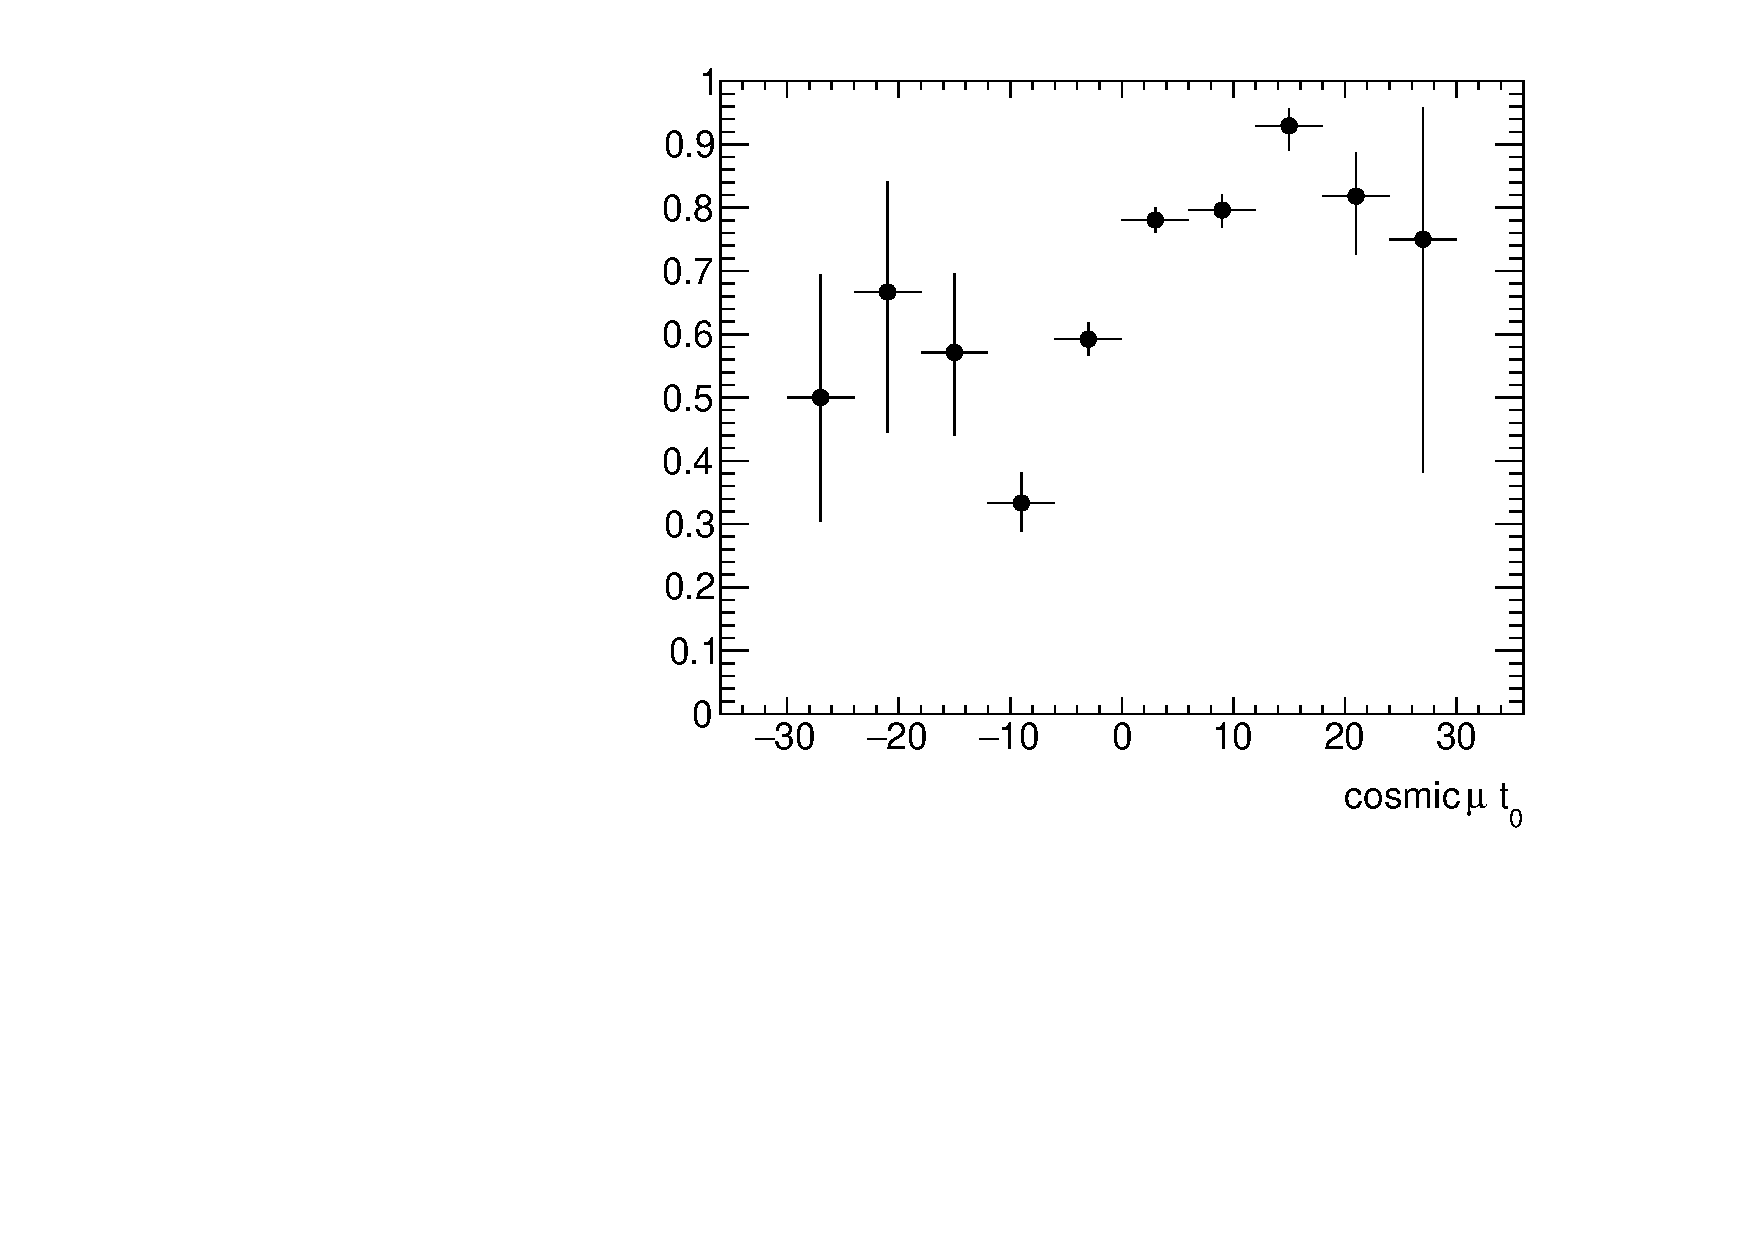
\includegraphics[width=.3\textwidth]{figures/LRT_systs/cosmics_phil0_eff_t0.pdf}
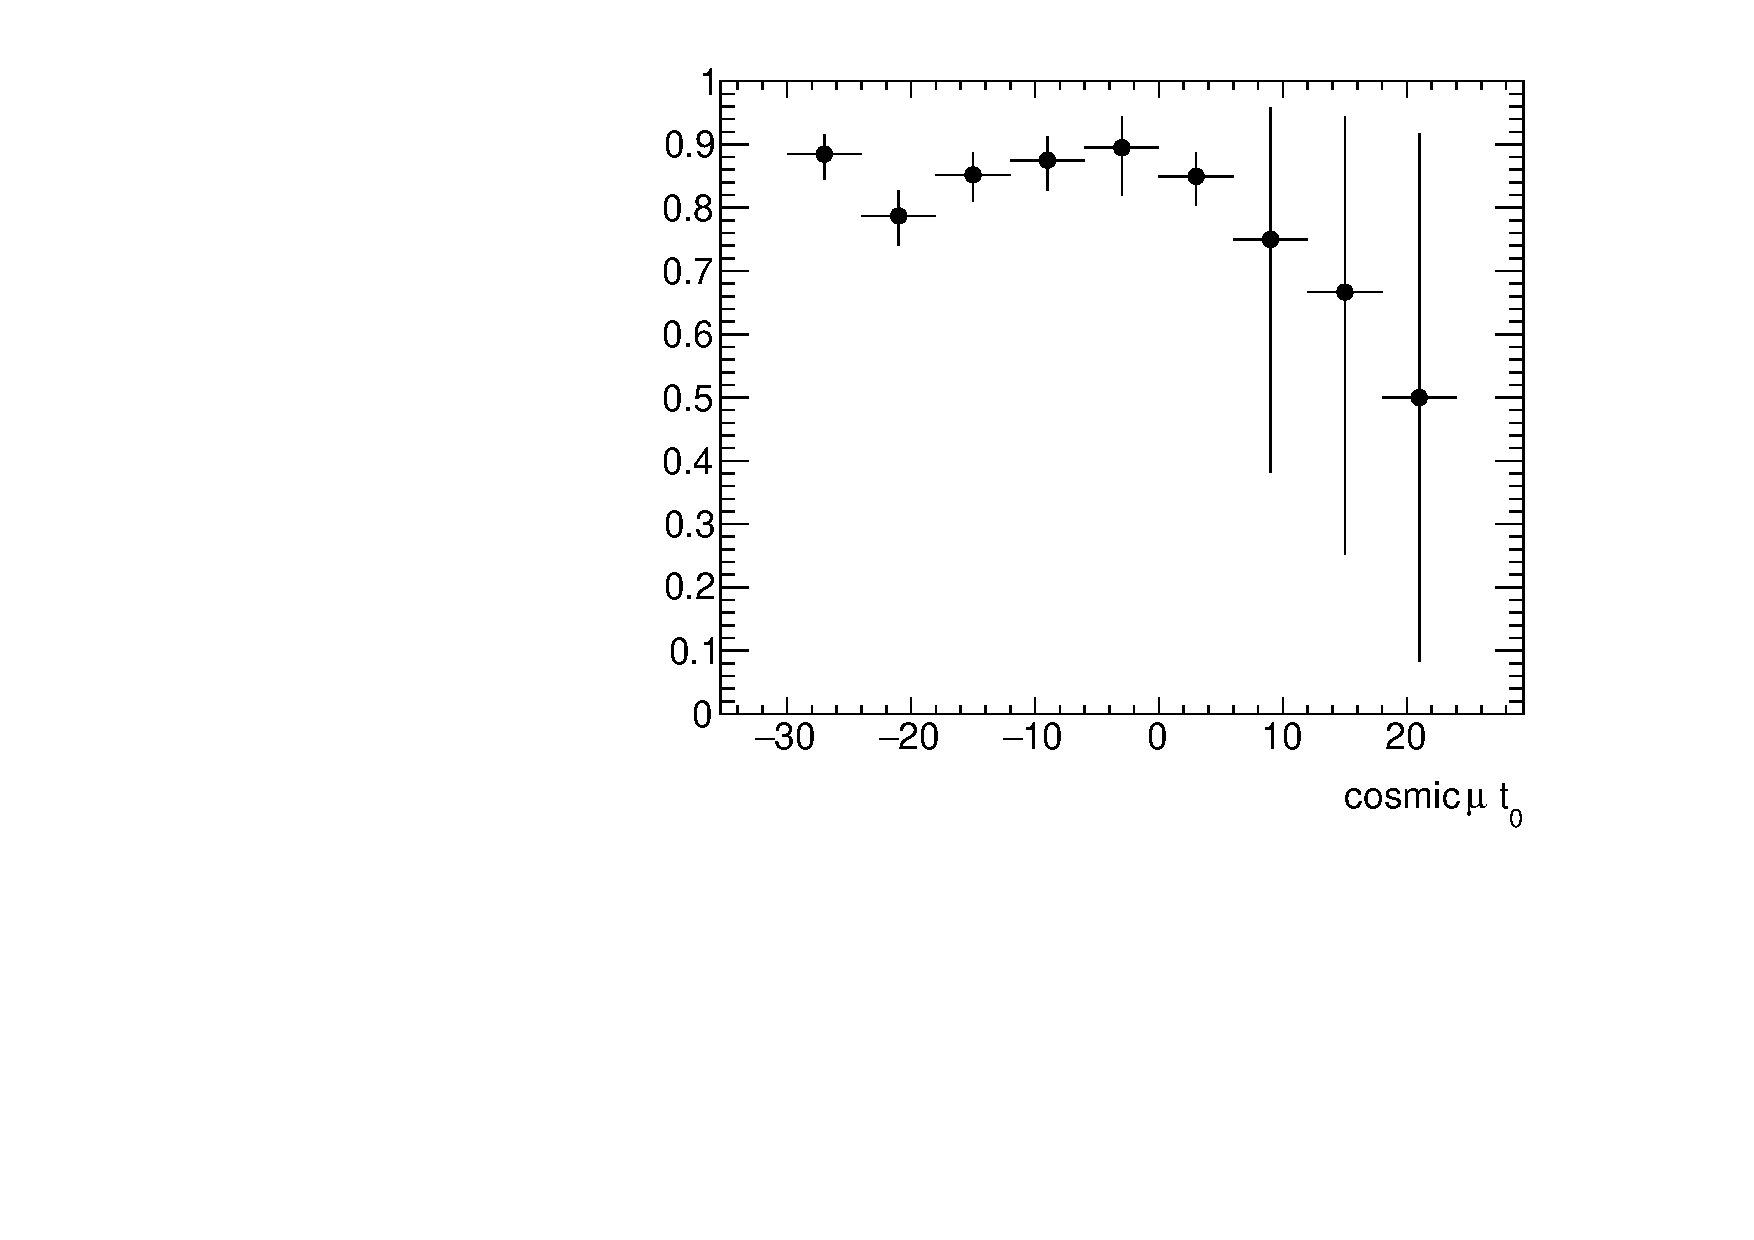
\includegraphics[width=.3\textwidth]{figures/LRT_systs/cosmics_phig0_eff_t0.pdf}
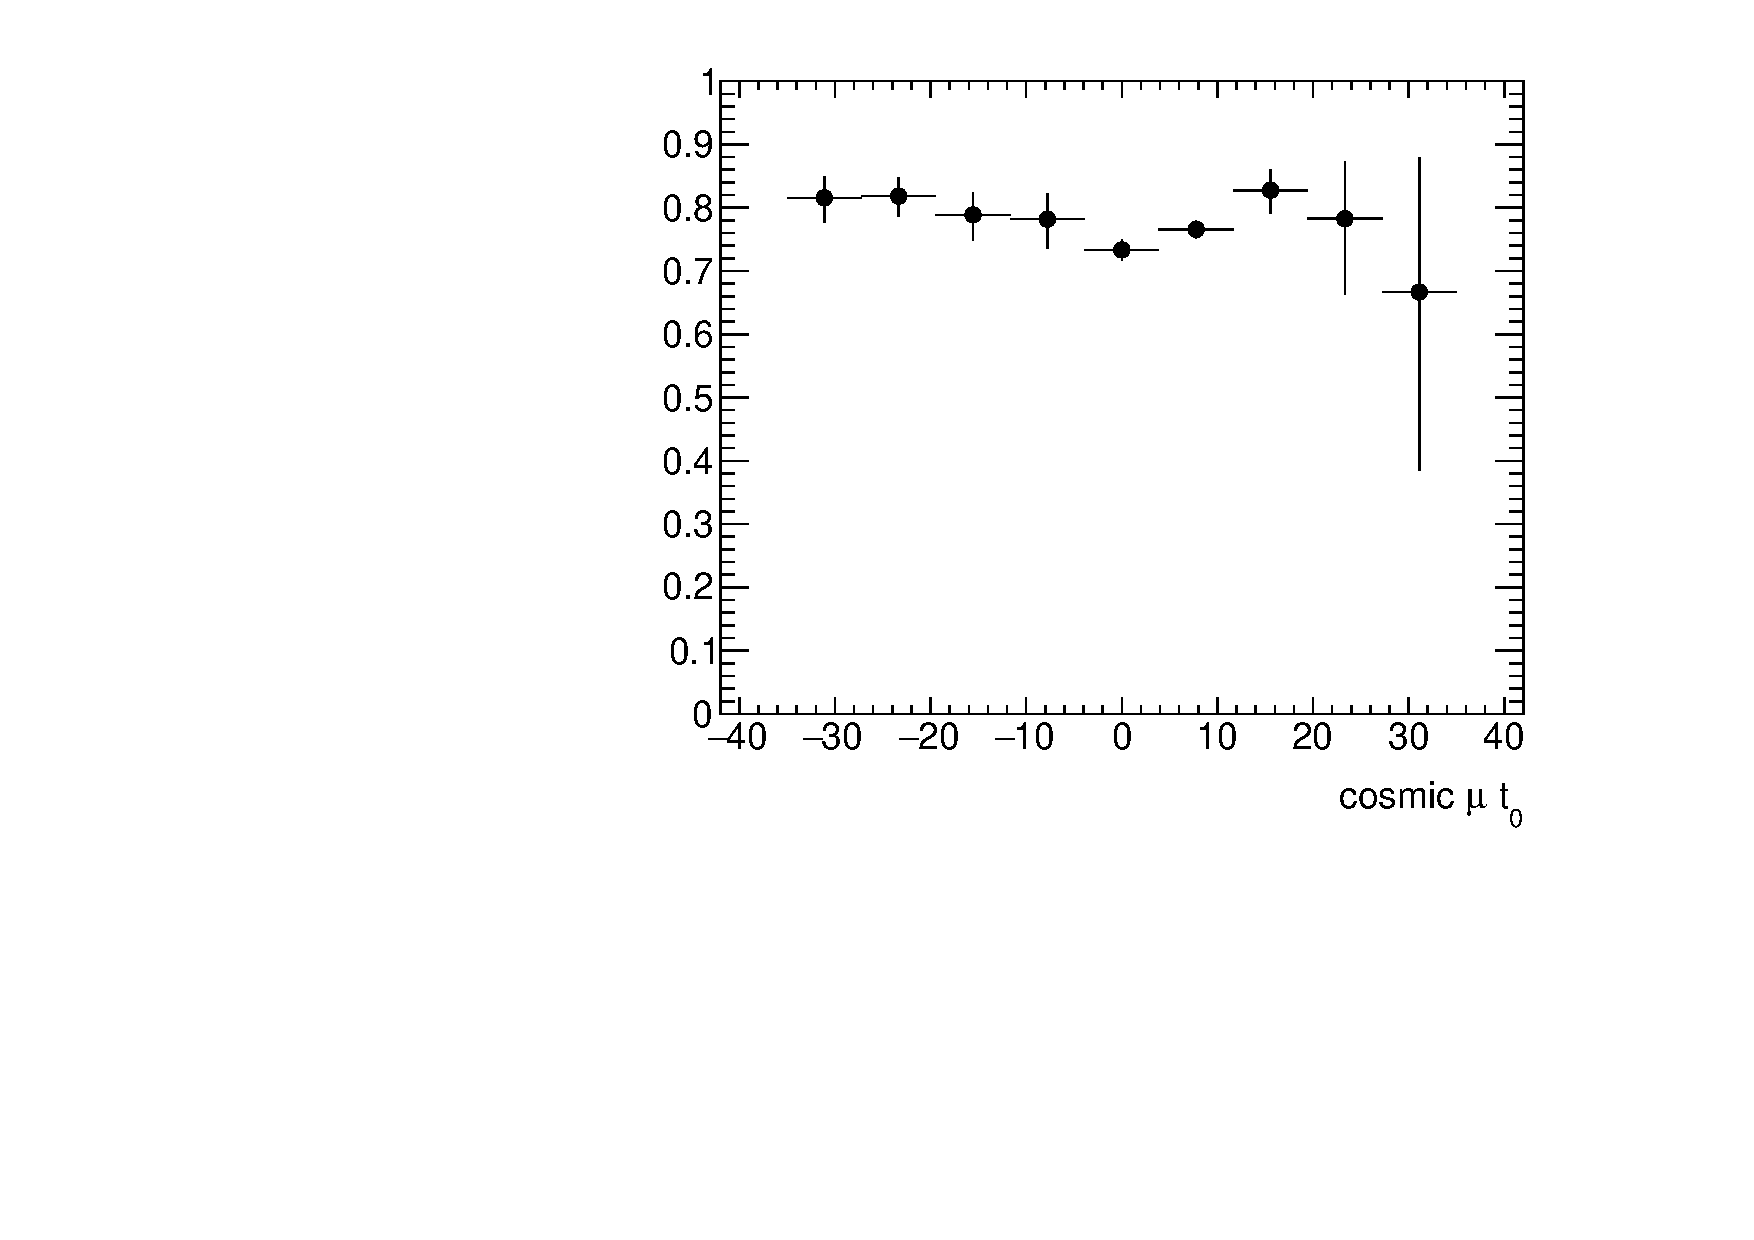
\includegraphics[width=.3\textwidth]{figures/LRT_systs/cosmics_eff_t0.pdf}
\caption{\ac{LRT} efficiency measured with various $\phi$ and \tavg cuts. The right shows $\phi < 0$ muons with no \tavg cut, the center shows $\phi > 0$ muons with no \tavg cut, and the left shows the final selections, with $\phi > 0$ requried to have \tavg < 0 and $\phi < 0$ \tavg > 0. This gives a consistent readout configuration and an approximately flat efficiency w.r.t \tavg. In particular, there $\phi < 0$ muons with negative timing that result in an artificially low efficiency, likely due to incomplete readout.}
\label{fig:cos_sys_t0}
\end{figure}


\begin{figure}[htbp]
\centering
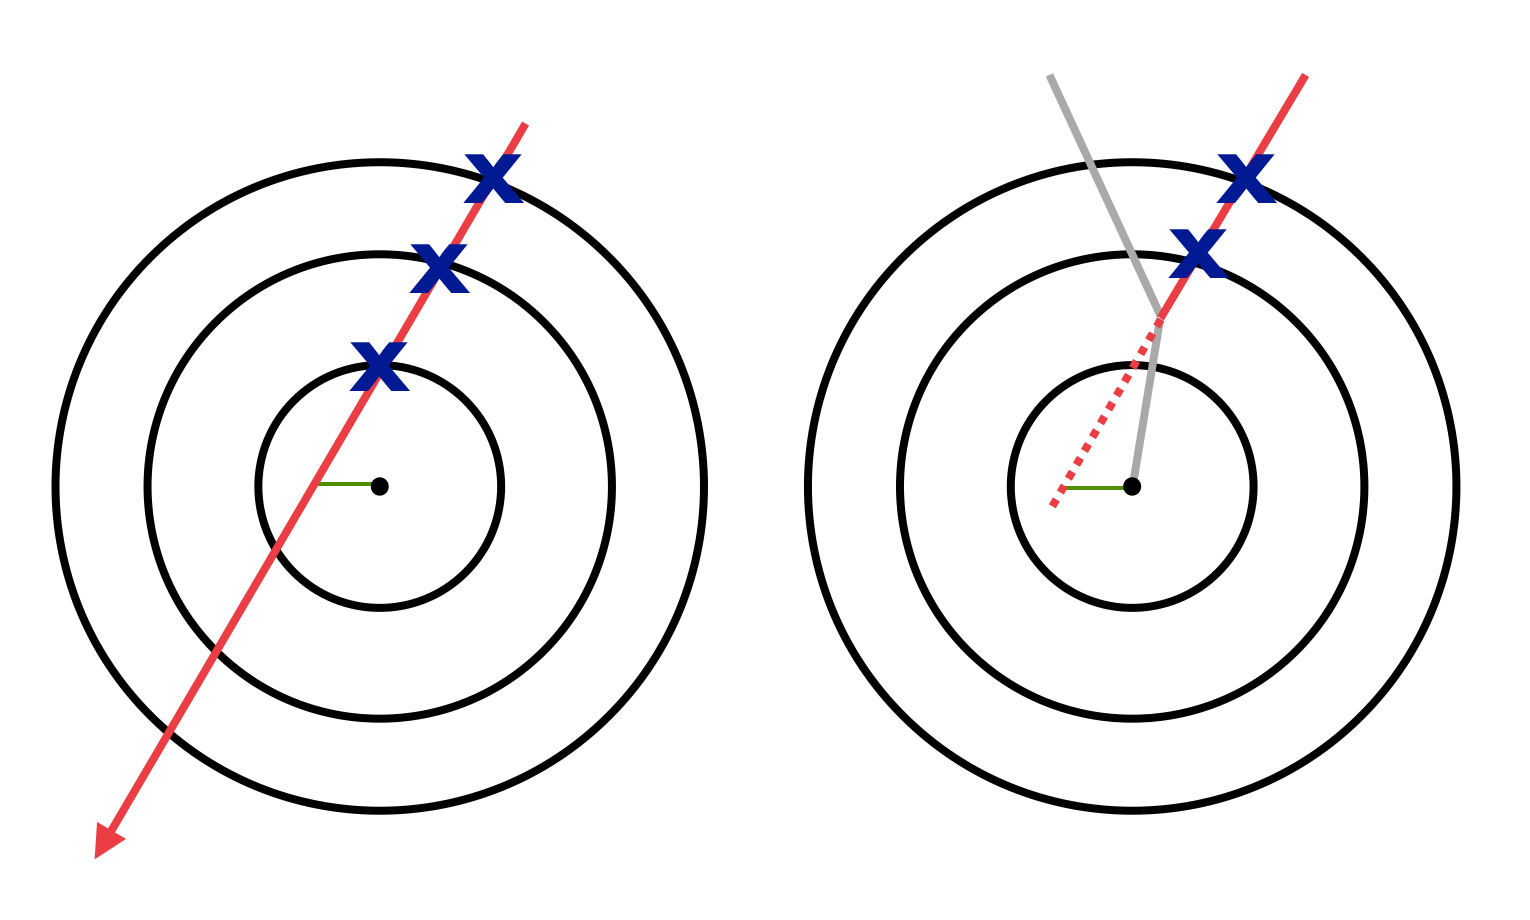
\includegraphics[width=.6\textwidth]{figures/LRT_systs/cos_sig_LRT.png}
\caption{An illustration of the difference in \dz measurements between cosmic (left) and signal muons. The \dz of a cosmic muon is always measured just before its first hit, whereas for a signal muon, the first hit can come far after the \dz. The blue x's represent \ac{ID} hits and the red lines represent muon tracks.}
\label{fig:lrt_sig_sketch}
\end{figure}


\begin{figure}[htbp]
\centering
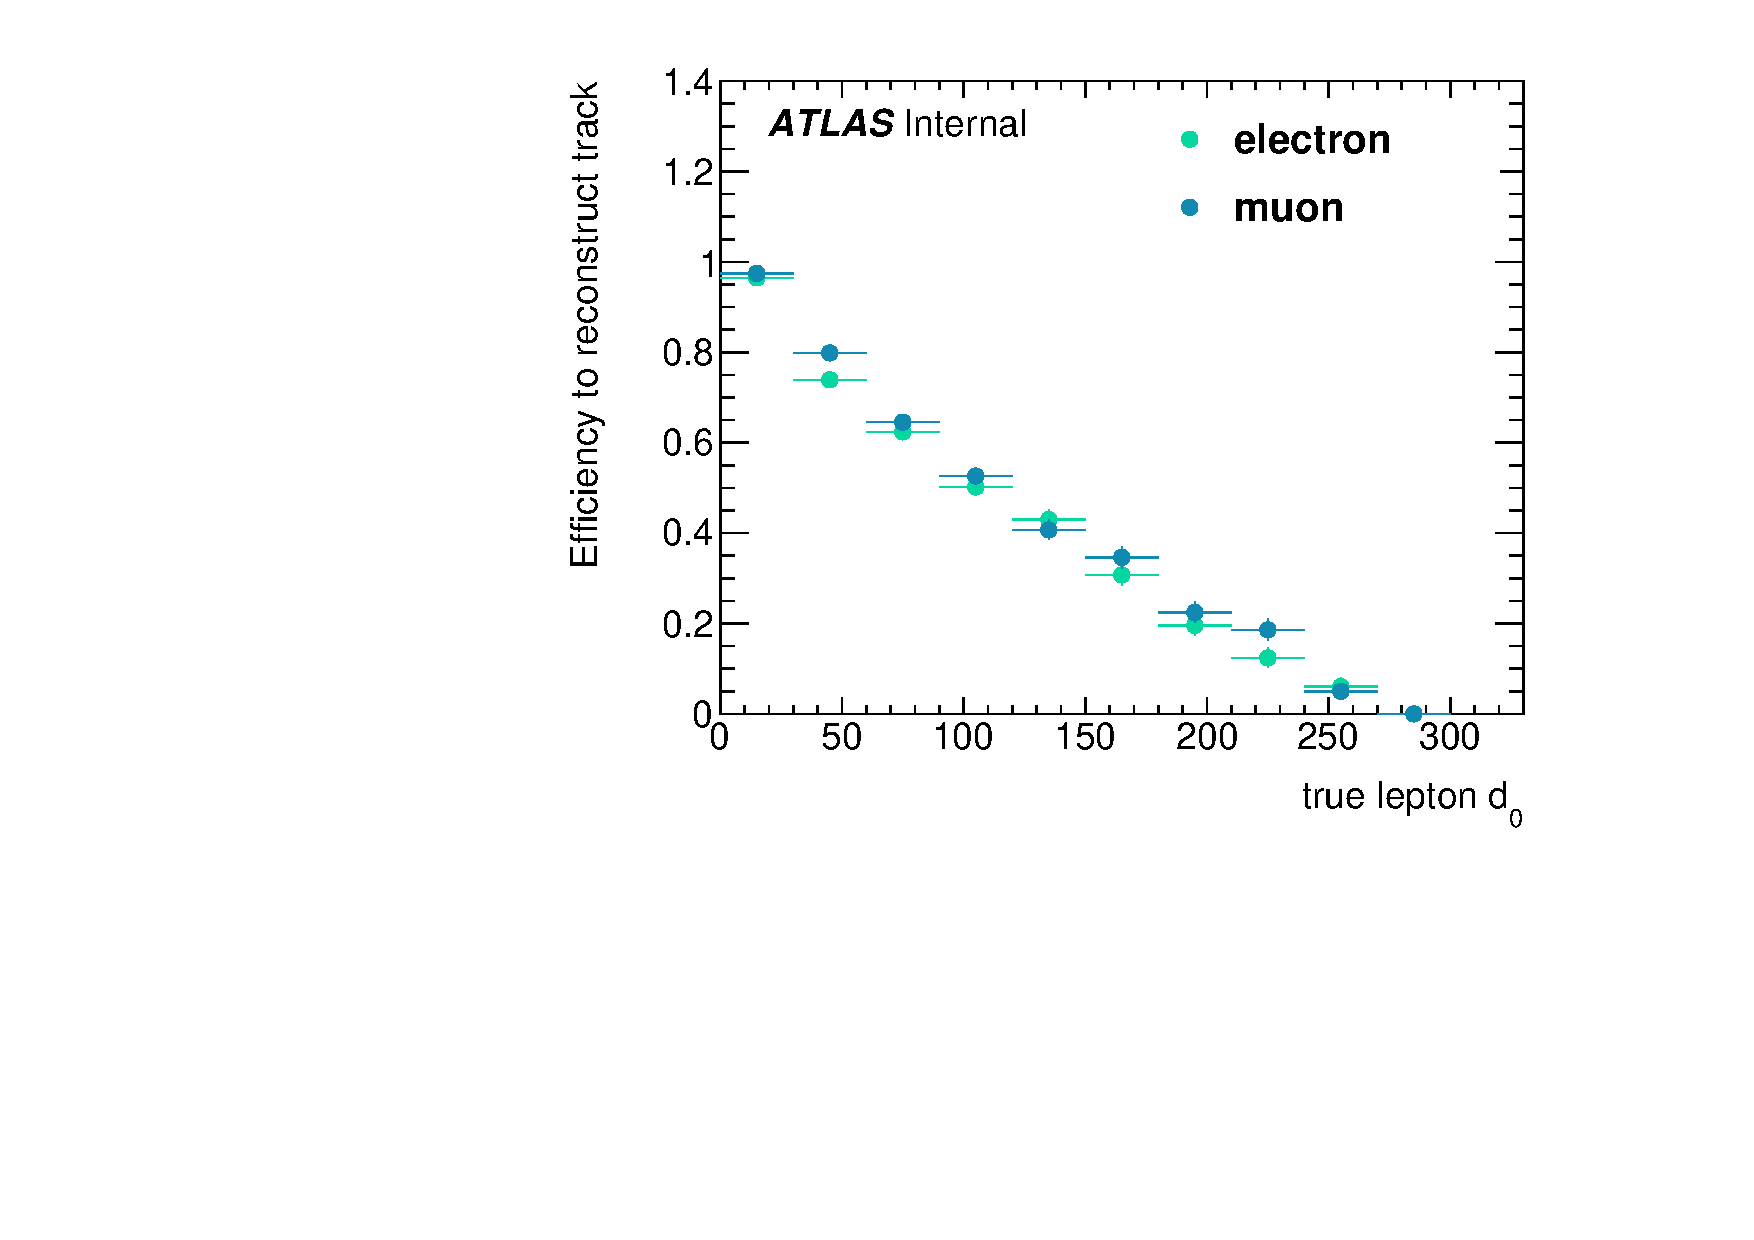
\includegraphics[width=.48\textwidth]{figures/LRT_systs/stlrt_compare_elmu_d0.pdf}
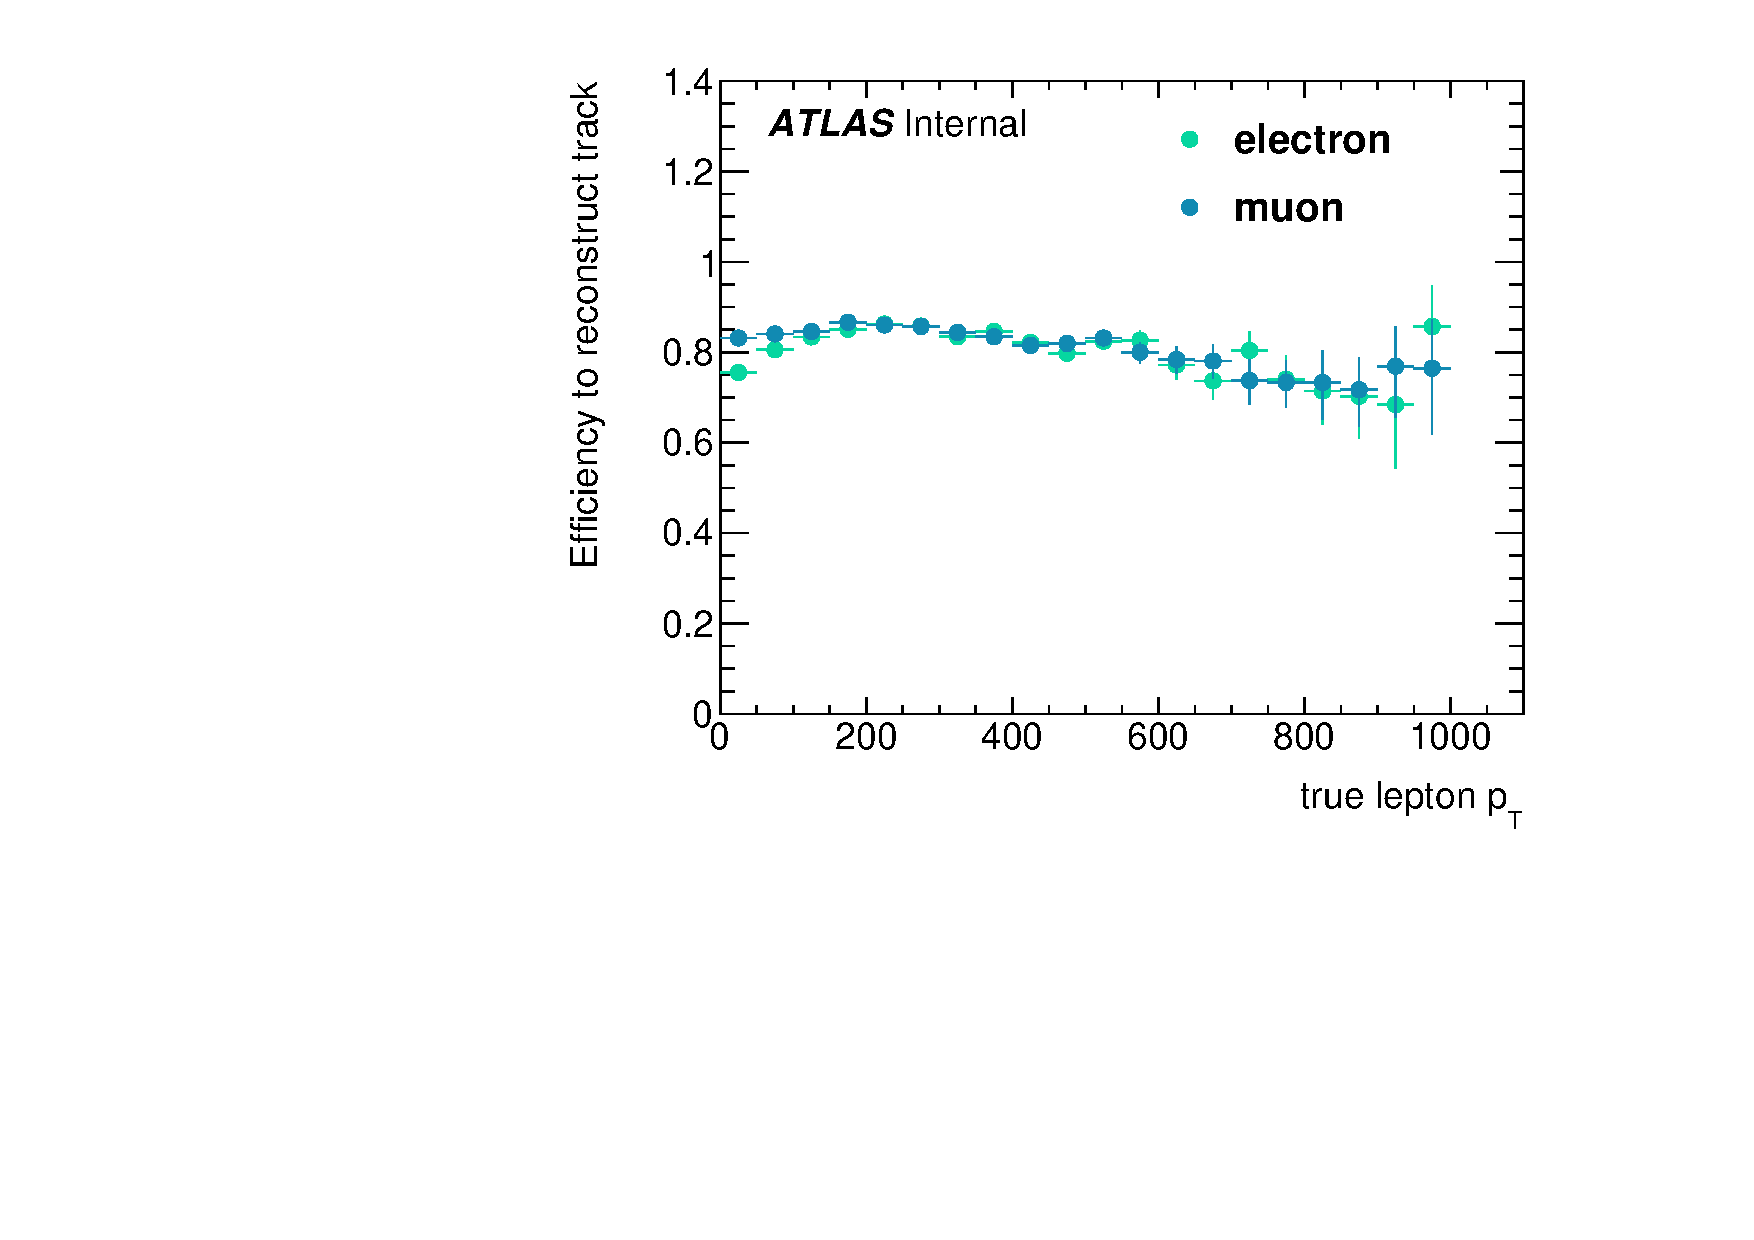
\includegraphics[width=.48\textwidth]{figures/LRT_systs/stlrt_compare_elmu_pt.pdf}
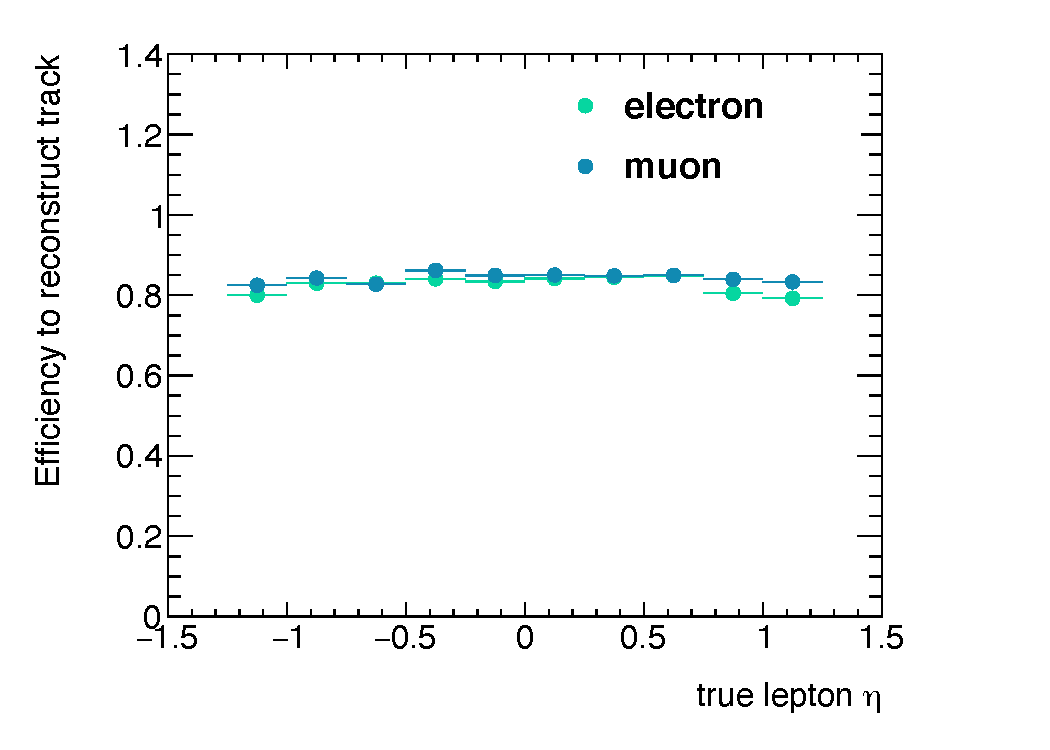
\includegraphics[width=.48\textwidth]{figures/LRT_systs/stlrt_compare_elmu_eta.pdf}
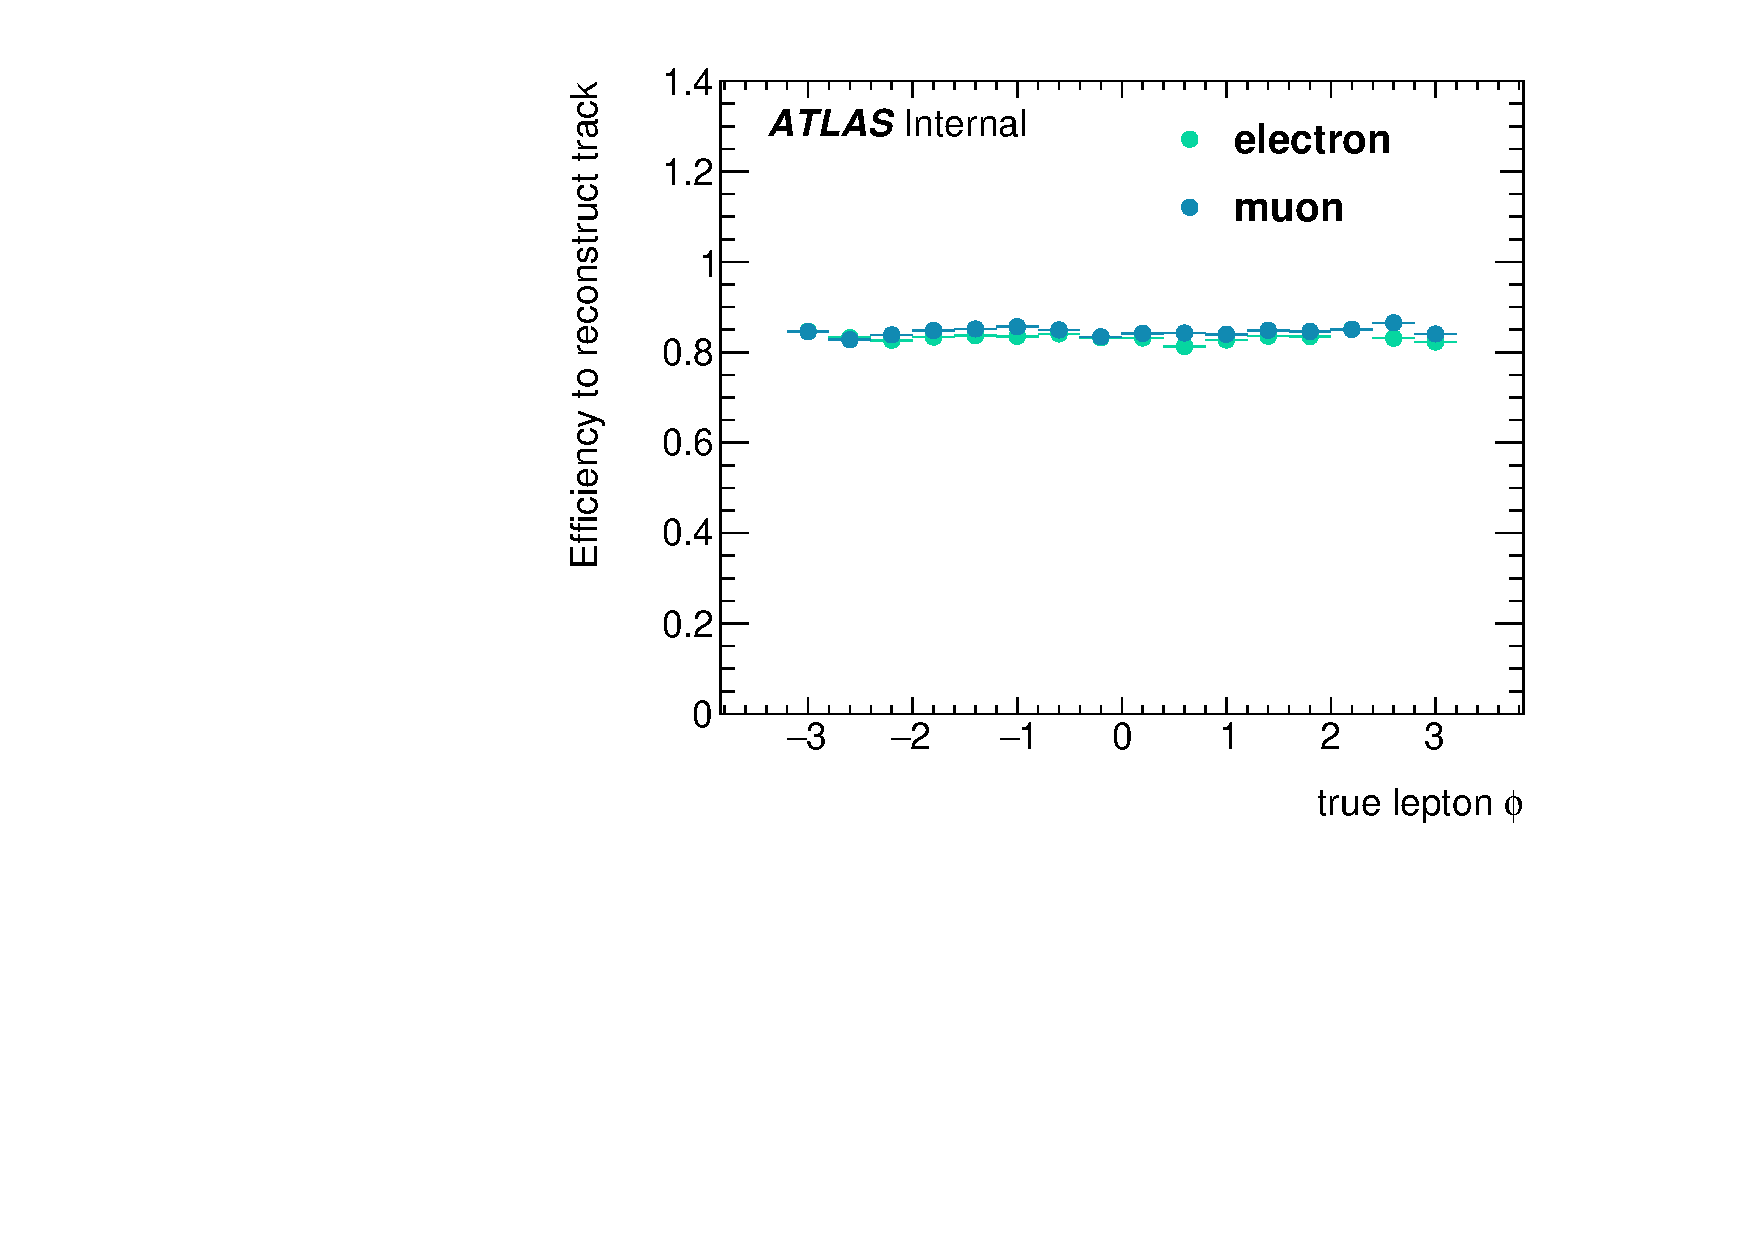
\includegraphics[width=.48\textwidth]{figures/LRT_systs/stlrt_compare_elmu_phi.pdf}
\caption{Tracking efficency for electrons and muons in signal MC (all lifetimes of 300 GeV slepton). These plots justify the assumpution that tracking efficiency is the same between electrons and muons and symmetric about the \ac{ID} volume.}
\label{fig:trk_el_mu}
\end{figure}

\begin{table}
\begin{tabular}{c}
Cut on cosmic muon \\
\hline
$\pt > 50 \GeV$ \\
$\absdz > 3$mm \\
$|\eta| < 1.05$ \\
$\absz < 120$ mm \\
$\tavg > 0$ if $\phi_{\mu} < 0$ OR $\tavg > 0$ if $\phi_{\mu} > 0$ \\
\hline
\end{tabular}
\quad
\begin{tabular}{c}
Cut on truth muon\\
\hline
$\pt > 50 \GeV$ \\
$\absdz > 3$mm \\
$|\eta| < 1.05$ \\
parent is a slepton \\
\dz and $R_{\textrm{decay}}$ between the same silicon layers\\
\hline
\end{tabular}
\caption{Cuts on tag muons. Cosmic muons (right) and truth signal muons (left).}
\label{tab:lrt-mu-cuts}
\end{table}

\begin{table}
\centering
\begin{tabular}{c}
Cut on cosmic muon \\
\hline
$\pt > 30 \GeV$ \\
$\Delta R_{\textrm{cos}}= \sqrt{ (\Delta \phi - \pi)^{2} + (\Sigma \eta)^{2}} < 0.3$ \\
$|d_{0, \textrm{track}} - d_{0, \mu}| < 20$ \\
$|z_{0, \textrm{track}} - z_{0, \mu}| < 20$ \\
\hline
\end{tabular}
\quad
\quad
\begin{tabular}{c}
Cut on truth muon\\
\hline
$\pt > 30 \GeV$ \\
$\Delta R = \sqrt{ (\Delta \phi)^{2} + (\Delta \eta)^{2}} < 0.05$ \\
 \\
 \\
\hline
\end{tabular}
\caption{Cuts on probe \ac{ID} tracks. In data (right) and signal (left).}
\label{tab:lrt-track-cuts}
\end{table}



\begin{figure}[htbp]
\centering
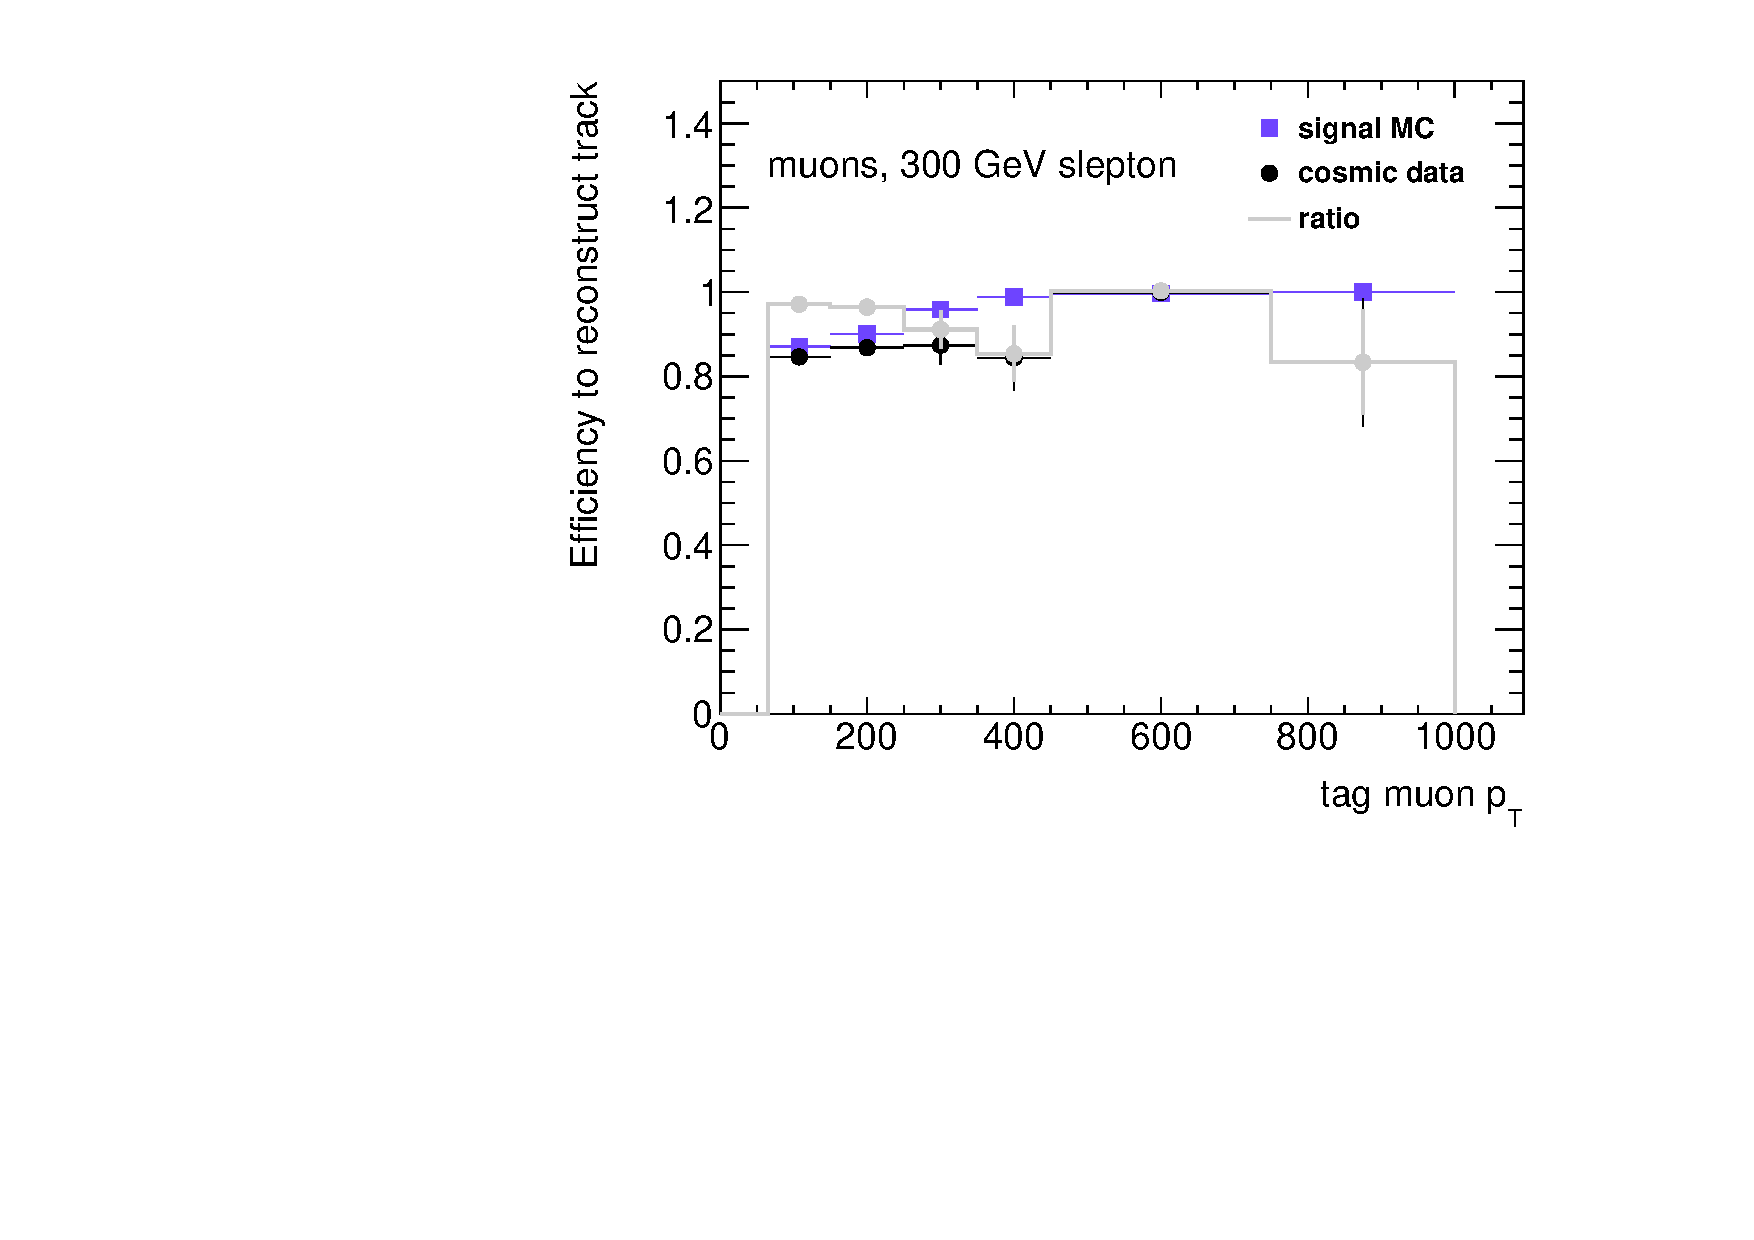
\includegraphics[width=.48\textwidth]{figures/LRT_systs/compare_pt_z0120_Rgd0_timing_idcuts_2dweight.pdf}
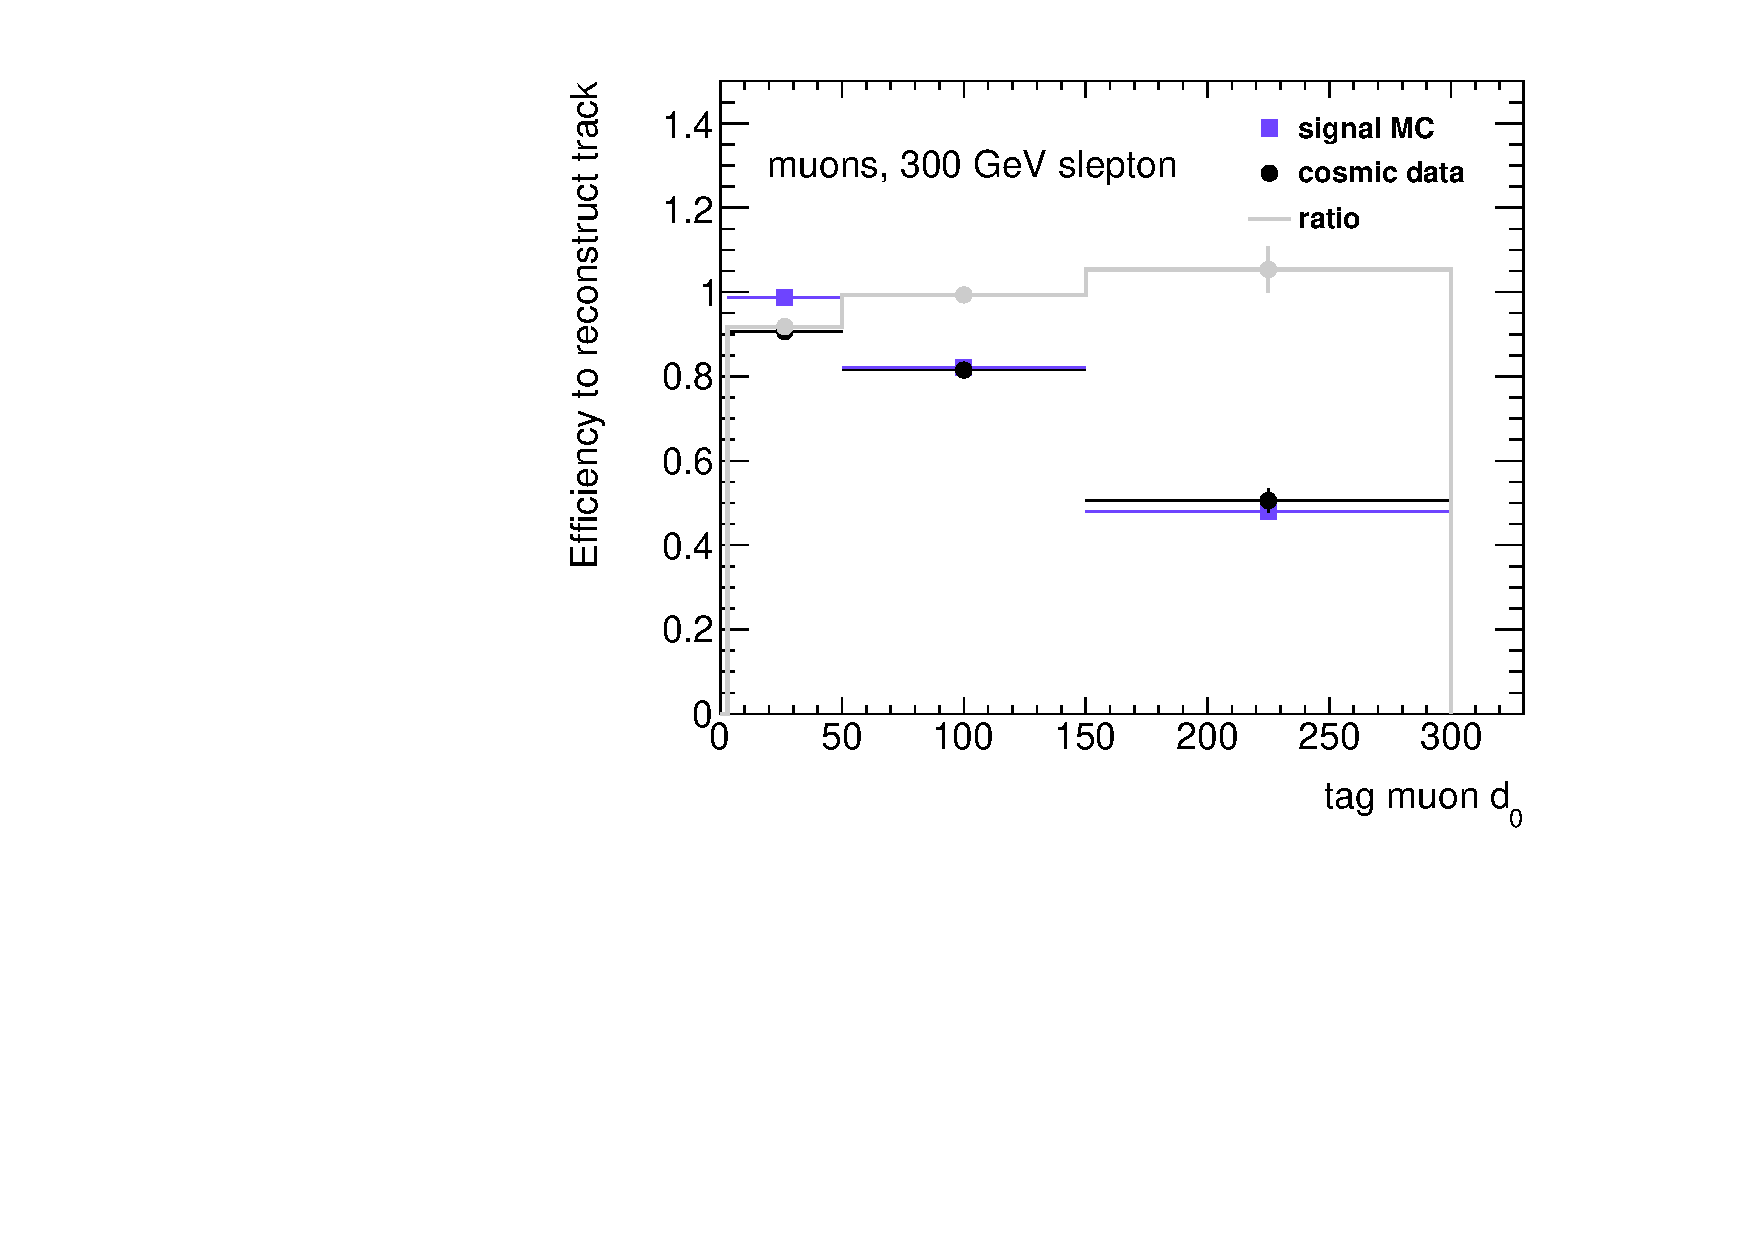
\includegraphics[width=.48\textwidth]{figures/LRT_systs/compare_d0_z0120_Rgd0_timing_idcuts_2dweight.pdf}
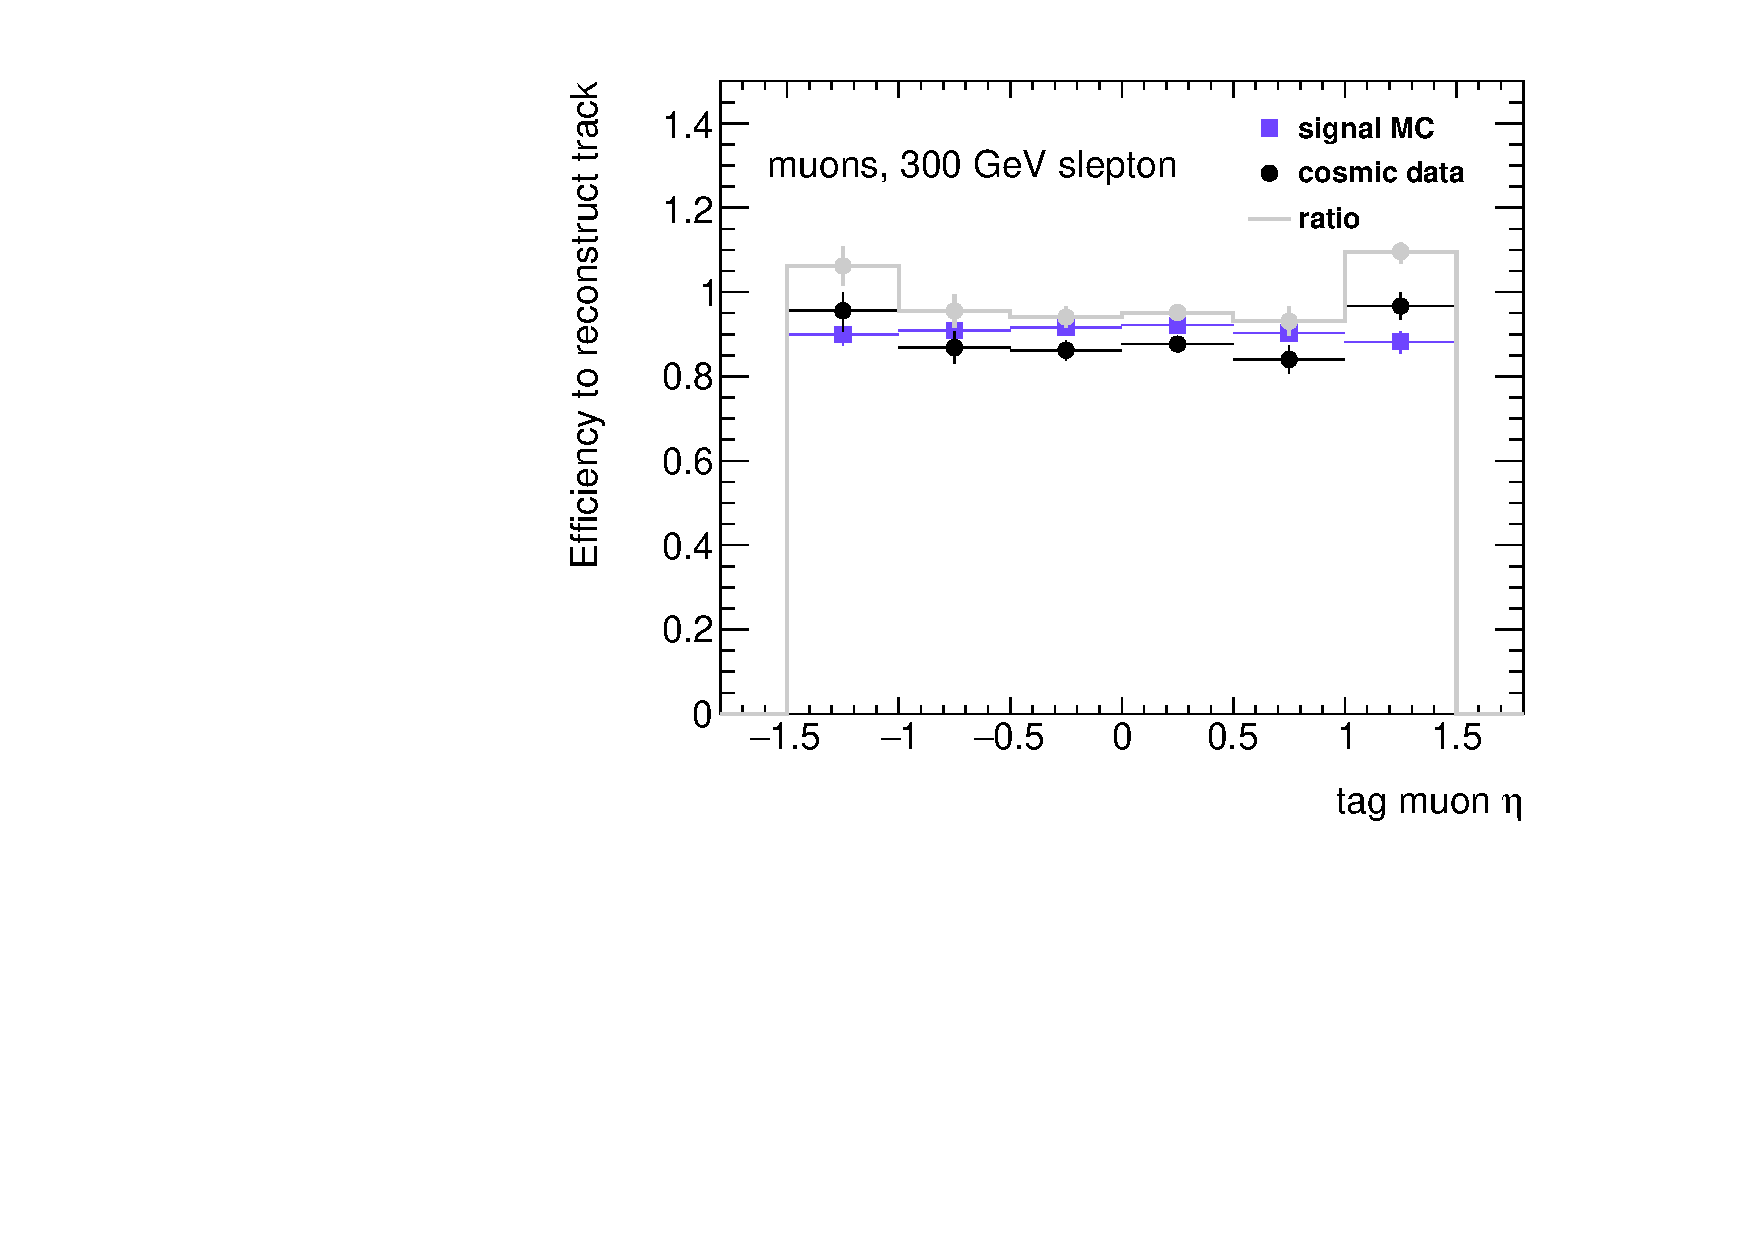
\includegraphics[width=.48\textwidth]{figures/LRT_systs/compare_eta_z0120_Rgd0_timing_idcuts_2dweight.pdf}
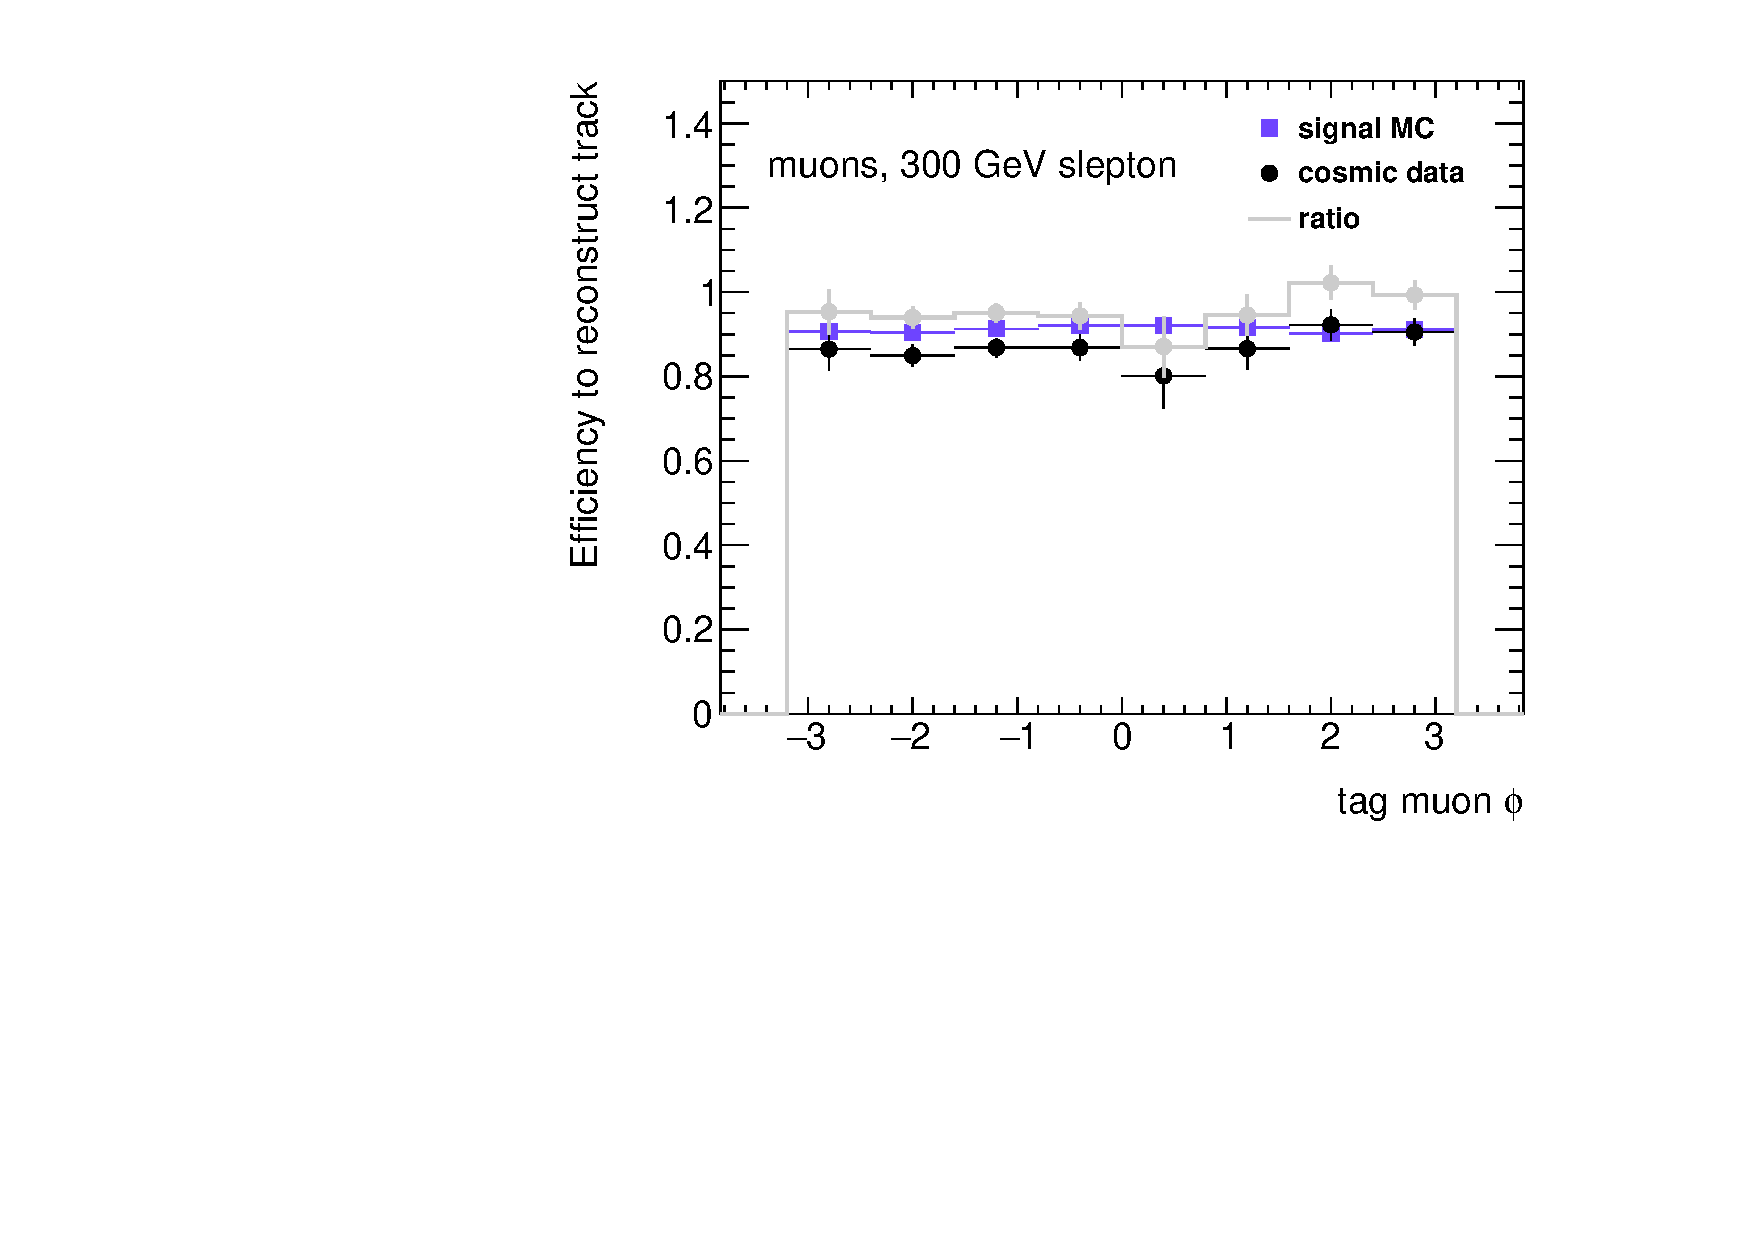
\includegraphics[width=.48\textwidth]{figures/LRT_systs/compare_phi_z0120_Rgd0_timing_idcuts_2dweight.pdf}
\caption{A comparison of tracking efficiency in cosmics data and signal MC (all masses and lifetimes can be used to due the eventual \pt and \dz binning) with respect to \pt (top left), \dz (top right), $\eta$ (bottom left), and $\phi$ (bottom right). The \ac{MC} efficiency is shown in purple, the data efficiency in black, and the ratio between the efficienceis is shown in gray.}
\label{fig:lrt_eff_comp}
\end{figure}

\begin{figure}[htbp]
\centering
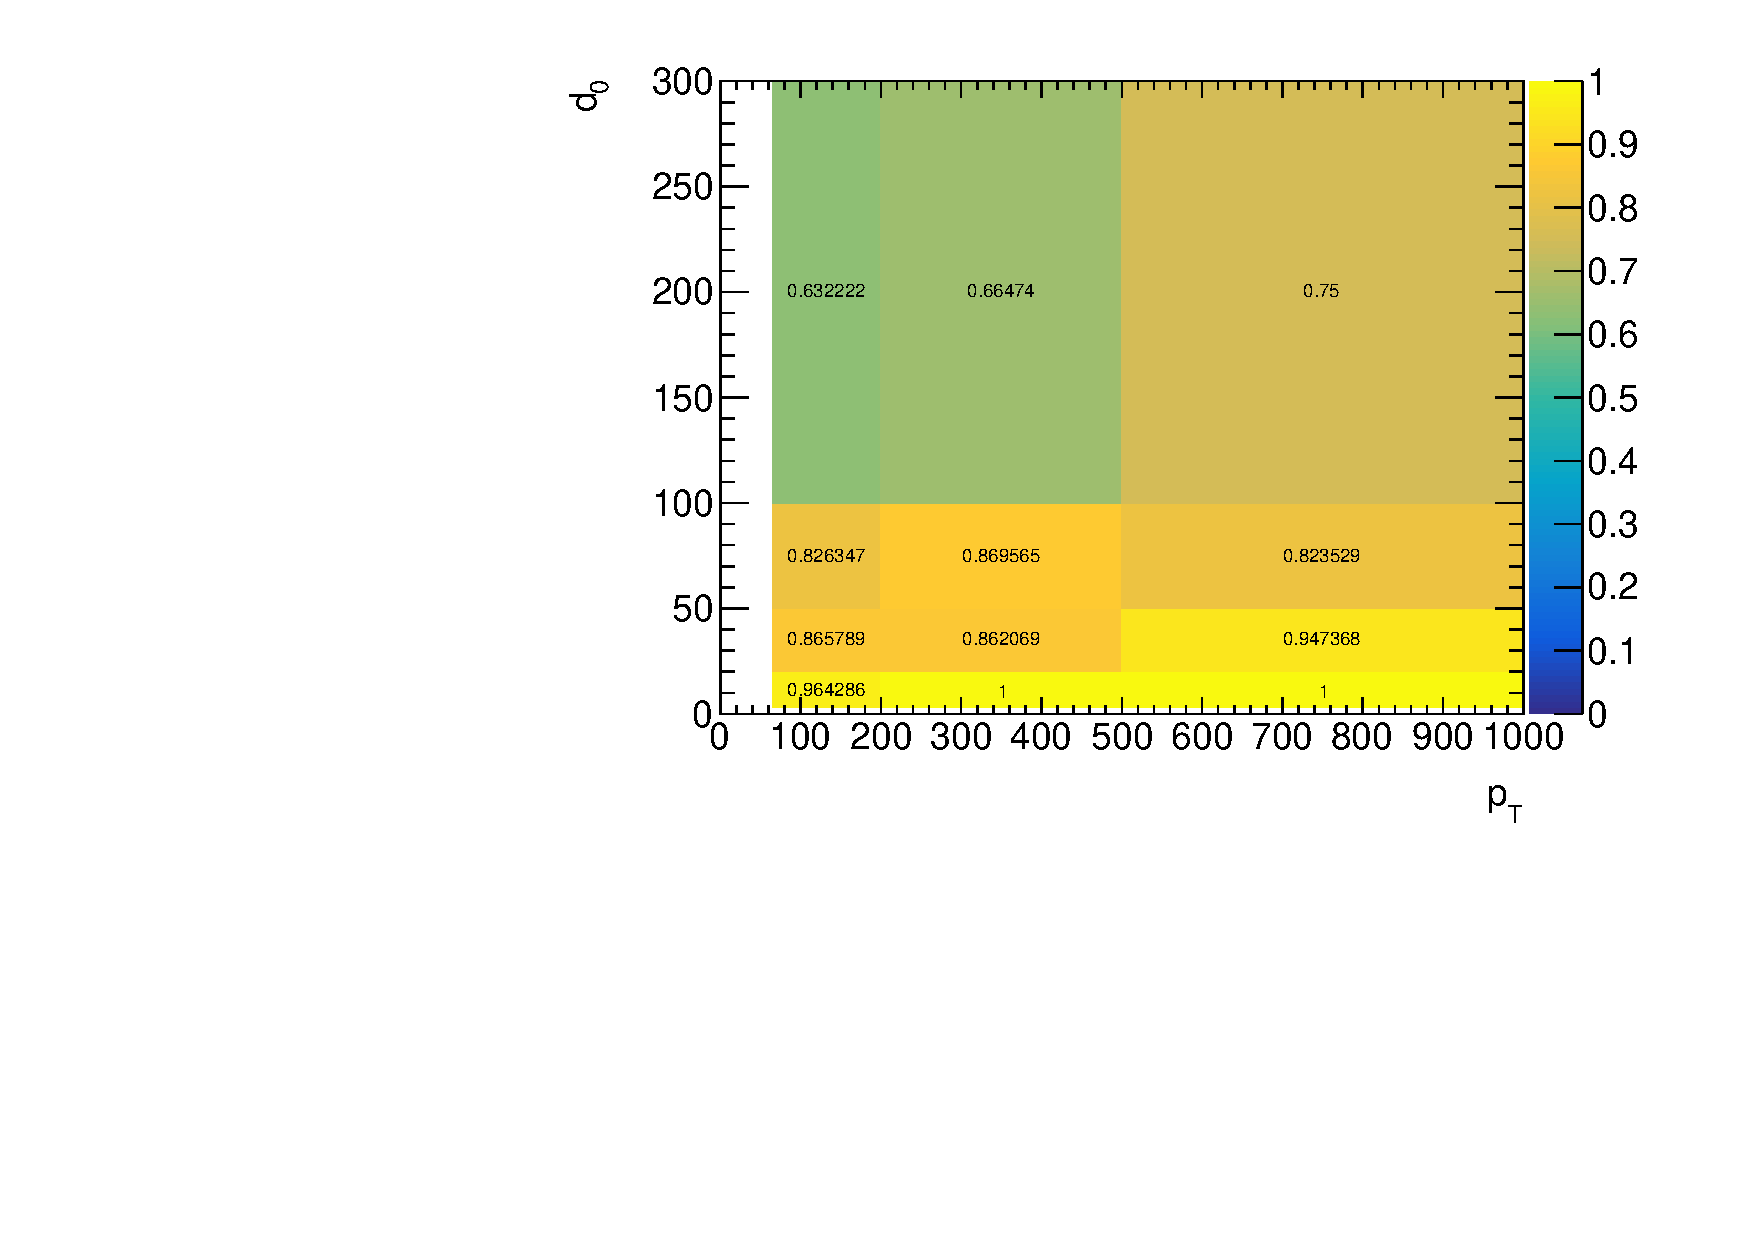
\includegraphics[width=.48\textwidth]{figures/LRT_systs/cosmics_rp3_dzp20_zzp20_z0120_Rgd0_timing_idcuts_eff_pt_d0.pdf}
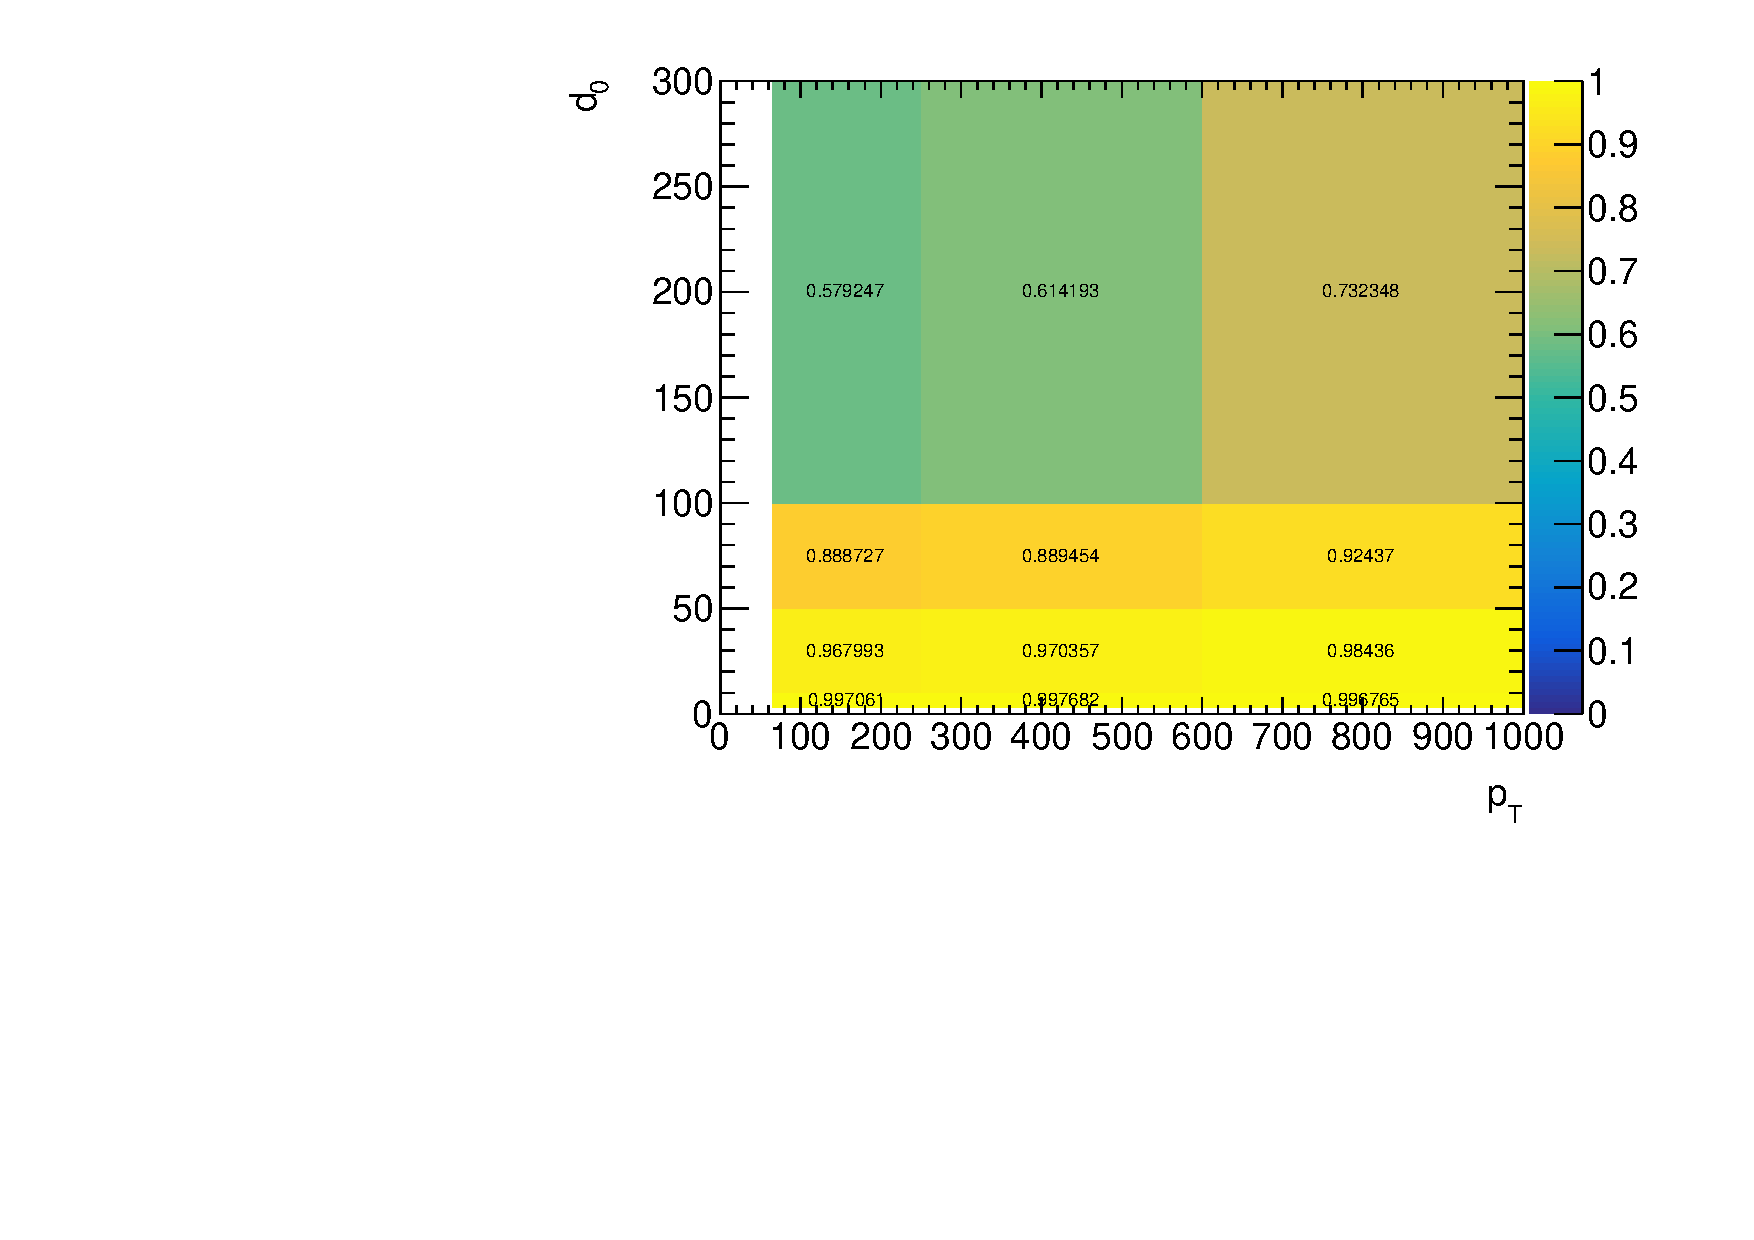
\includegraphics[width=.48\textwidth]{figures/LRT_systs/signal_eff_pt_d0_allmu_rp05_pt30_Rd0_allmass.pdf}
\caption{Tracking efficiency as a function of \pt and \dz in cosmics data (left) and MC before reweighting the cosmic \pt distribution. For MC, all masses and lifetimes of slepton signal are used.}
\label{fig:applrt_syst}
\end{figure}


\subsection{Lepton Displacement}

The effect of displacement on lepton reconstruction is applied as an additional uncertainty to account for reconstruction effects not captured by the tracking or prompt lepton systematic uncertainties. Specifically, this uncertainty is meant to capture any discrepancy in \ac{MS} track or electron shower shape parameters at high \absdz between data and MC, as well as how they are combined with the \ac{ID} track. Unfortunately, there is no sample high-\absdz leptons in data that can be used to compare to MC, so this uncertainty is conservatively defined as any change in efficiency with respect to prompt leptons. This uncertainty for muons is quite small, while it is much more substantial for electrons. Electrons are identified using a likelihood, which is trained with \dz as a discriminating variable. \absdz from the cuts performed offline, but the LH was not retrained, and so there as a larger relic \dz dependence and the displacement uncertainty is much larger. At high \absdz, the electron displacement uncertainty is dominant over the tracking uncertainty.

To determine the systematic uncertainty due to displaced reconstruction, we divide the baseline or signal reconstruction/selection efficiency by the tracking efficiency in order to separate any inefficiences from \ac{LRT}. Then, we take the ratio of each high \dz bin to the prompt bin (0-3mm), results of this are shown in Fig.~\ref{fig:disp_systs}. The uncertainty is assigned to each lepton and they are summed in quadrature to get an event level systematic. 

\begin{figure}[htbp]
\centering
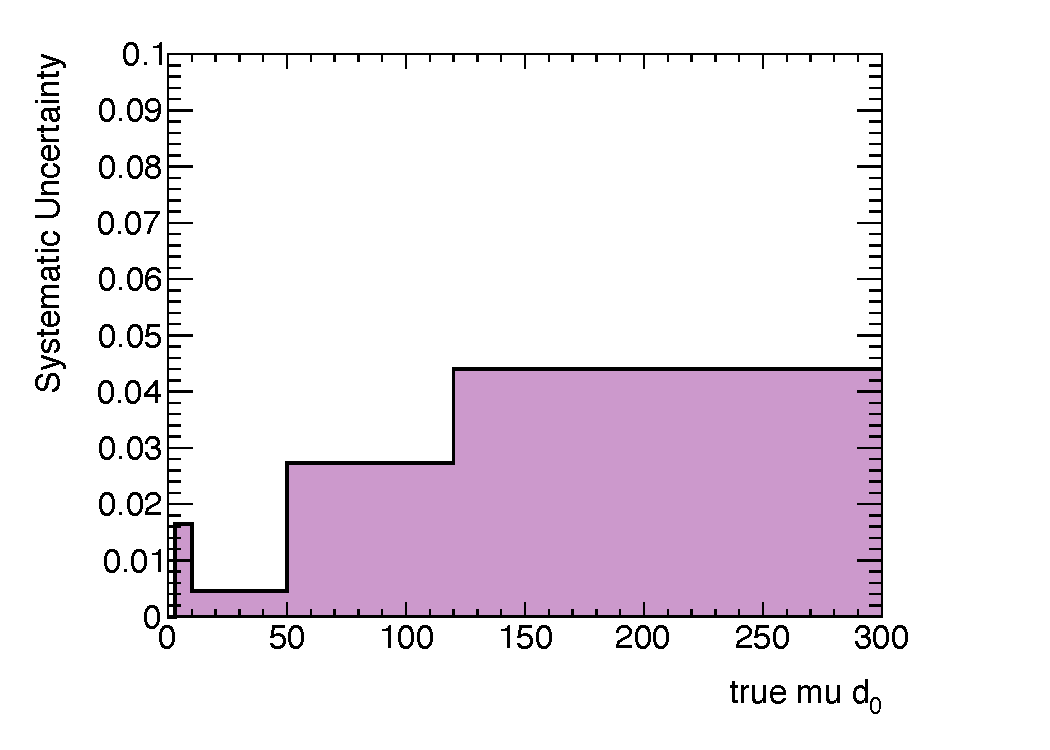
\includegraphics[width=.48\textwidth]{figures/disp_systs/signal_sf_d0_mu_300.pdf}
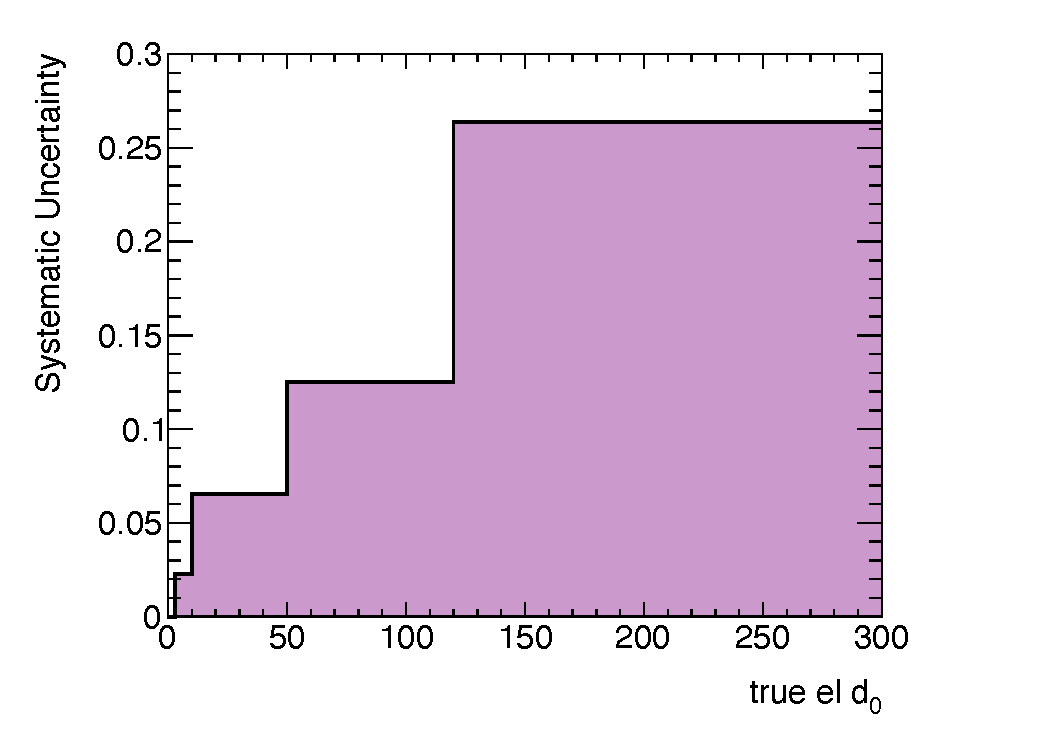
\includegraphics[width=.48\textwidth]{figures/disp_systs/signal_sf_d0_el_300.pdf}
\caption{Fractional systematic uncertainties defined for muons (left) and electrons. The value of each bin is defined as 1 minus the ratio of the selection efficiency with respect to tracking efficiency of the given bin to the same value of the prompt (0-3mm) bin. These are defined in the 300 GeV signal samples with lifetimes between 0.01ns-1ns. It was confirmed that the trends are consistent across various slepton masses.}
\label{fig:disp_systs}
\end{figure}

\begin{figure}[htbp]
\centering
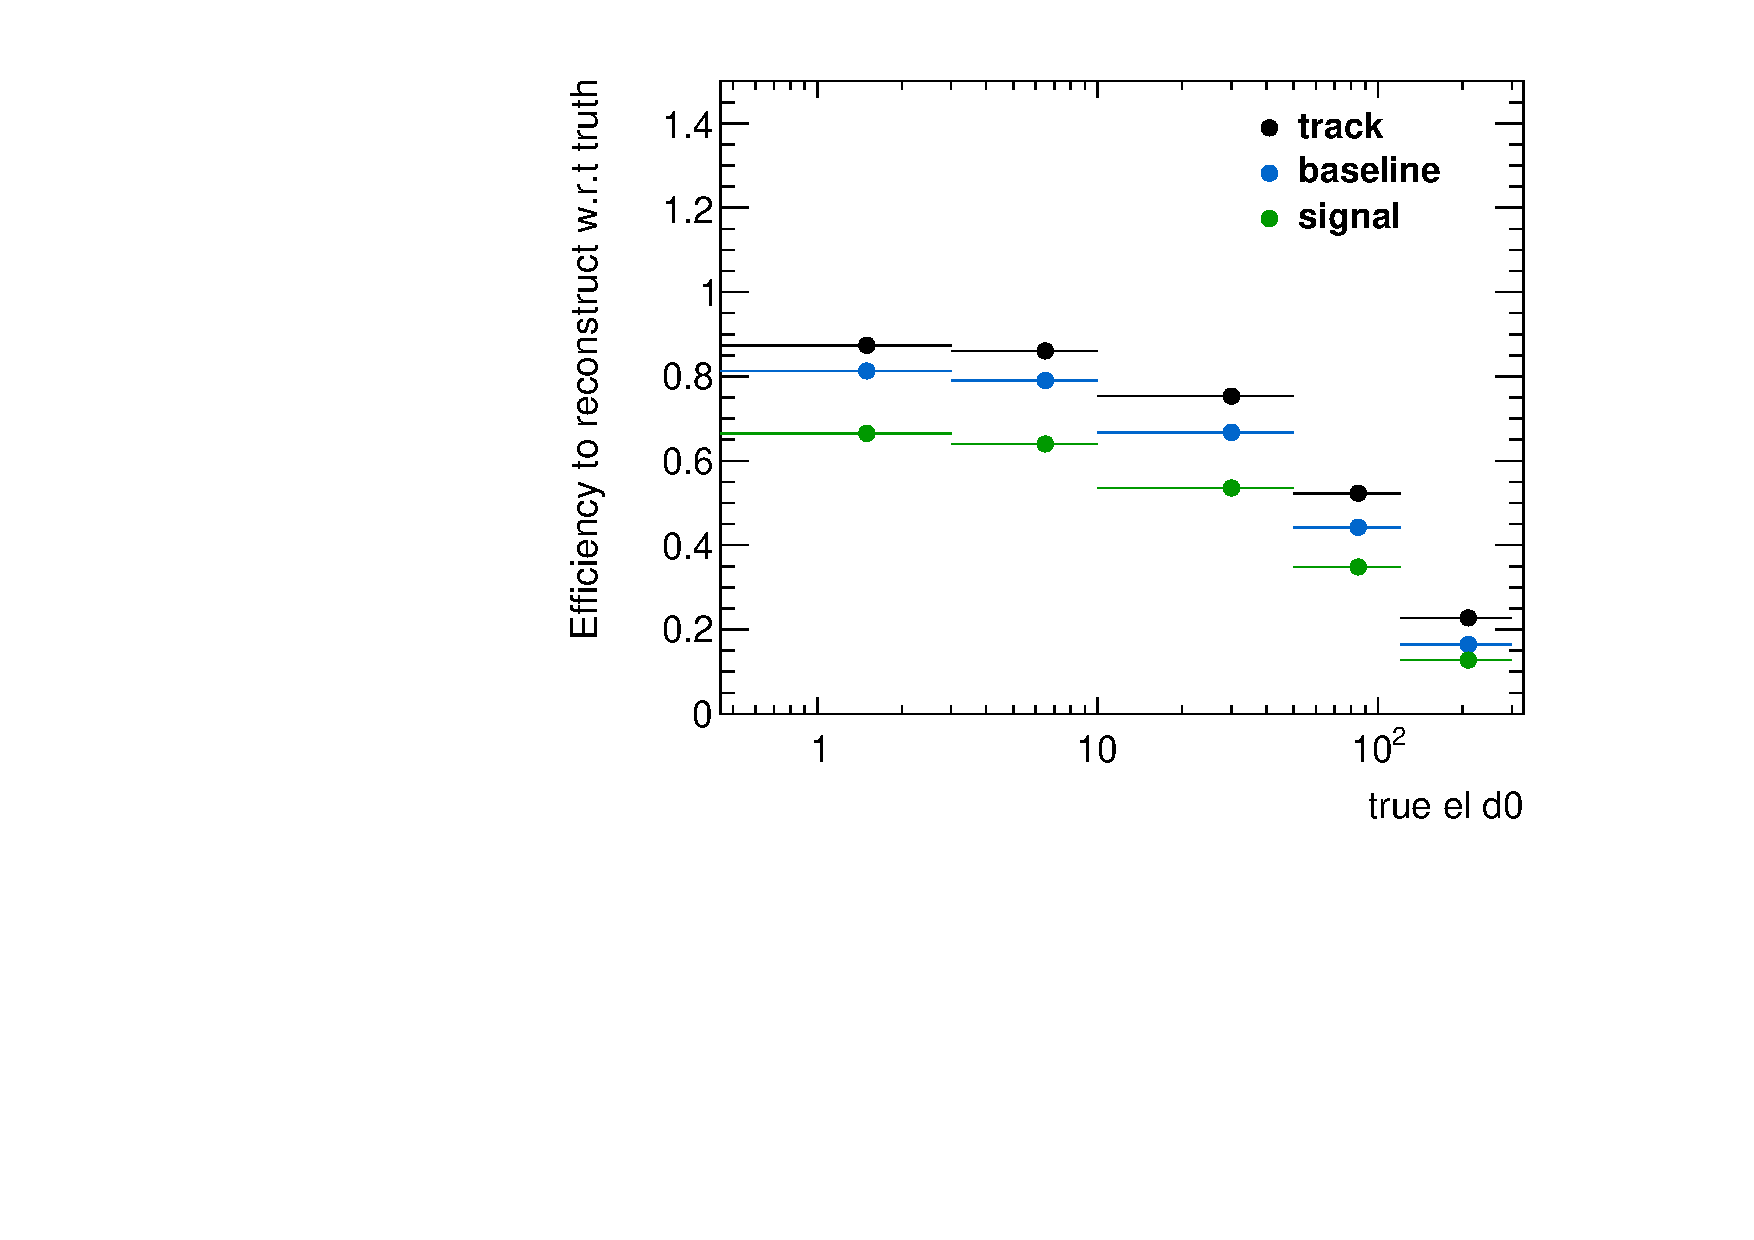
\includegraphics[width=.48\textwidth]{figures/disp_systs/signal_effcompare_d0_el_300.pdf}
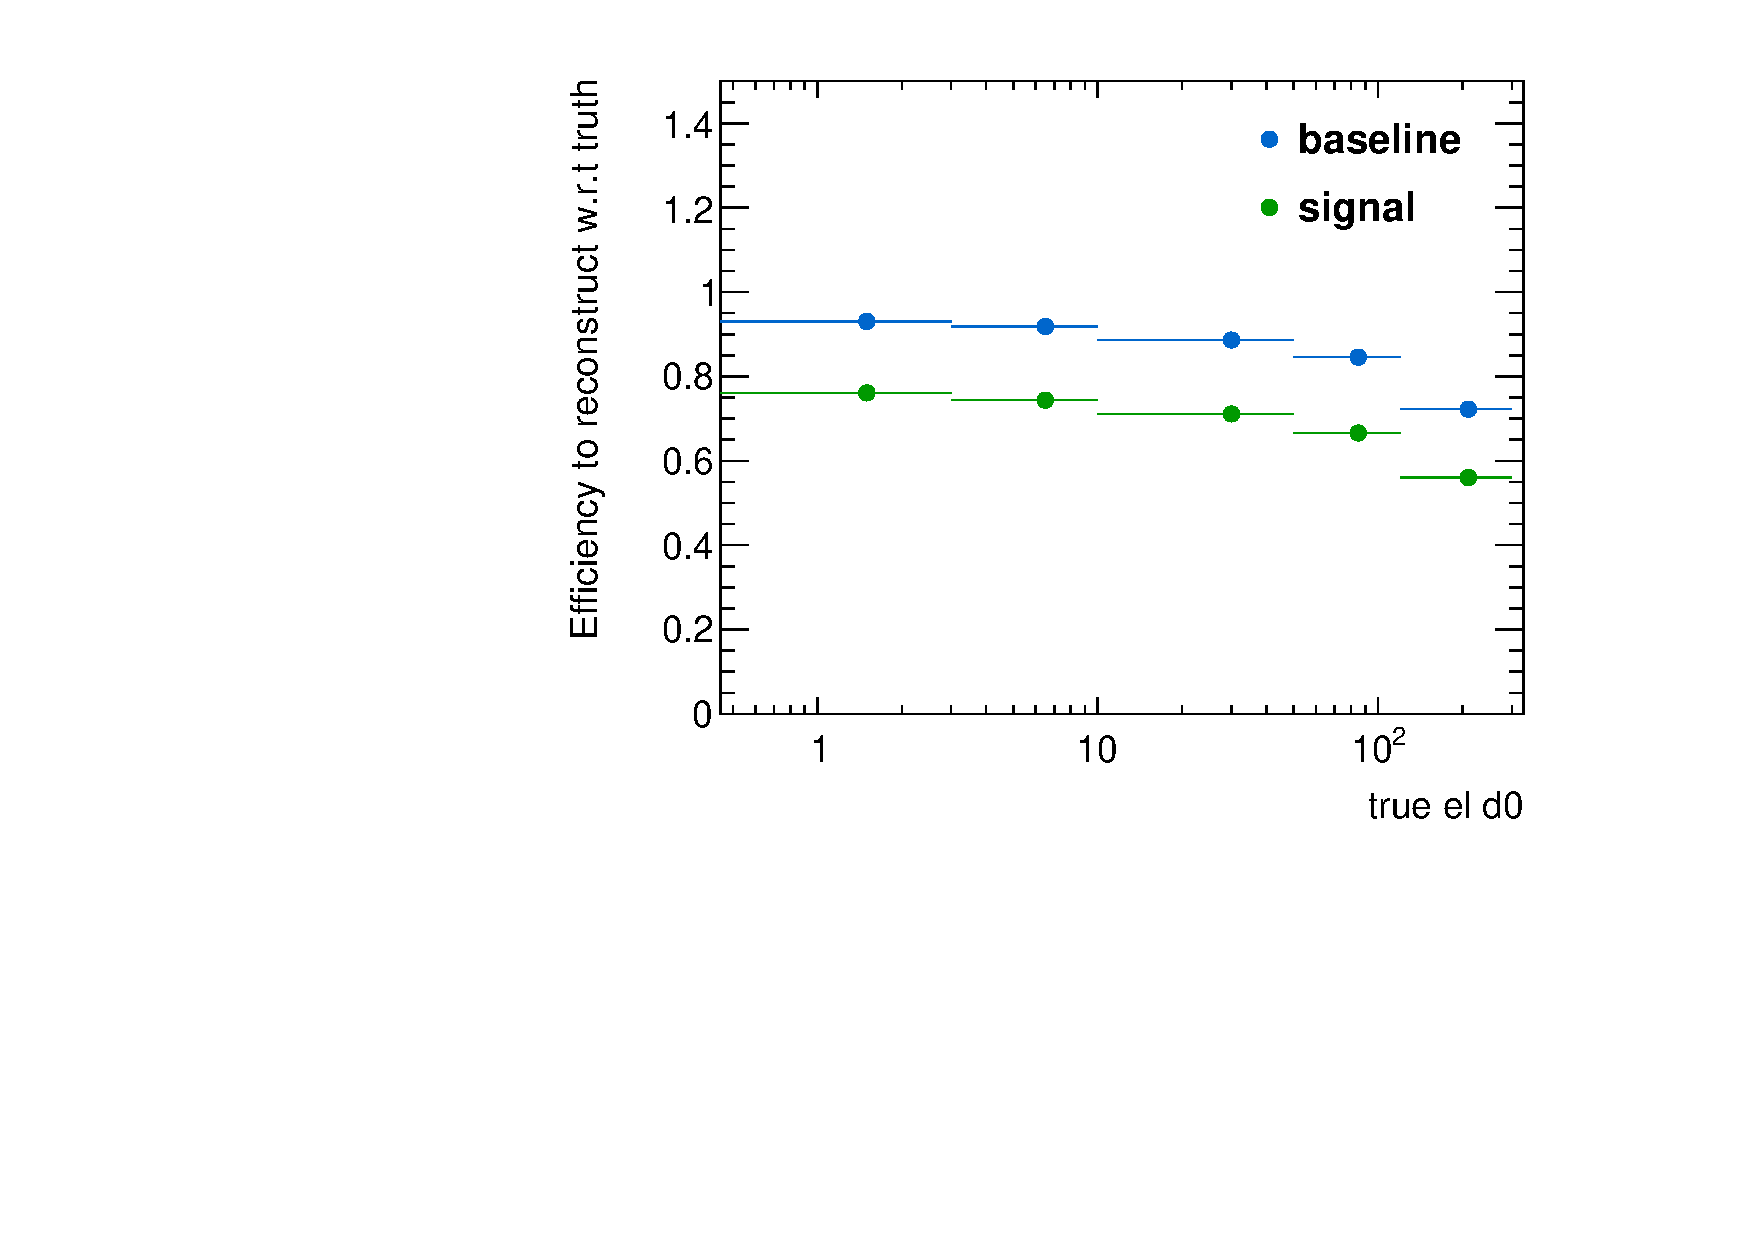
\includegraphics[width=.48\textwidth]{figures/disp_systs/signal_effwrttrack_d0_el_300.pdf}
\caption{Electron selection efficiencies with respect to truth (left) and with respect to the tracking efficiency (right). Made from a 300 GeV signal sample with lifetimes between 0.01ns-1ns. The denominator of the efficiency is truth electrons from sleptons with $\pt > 65 \GeV$ and $|\eta| < 2.5$, and the numerator is truth matched and signal (or baseline) quality tracks or leptons.}
\label{fig:disp_el}
\end{figure}

\begin{figure}[htbp]
\centering
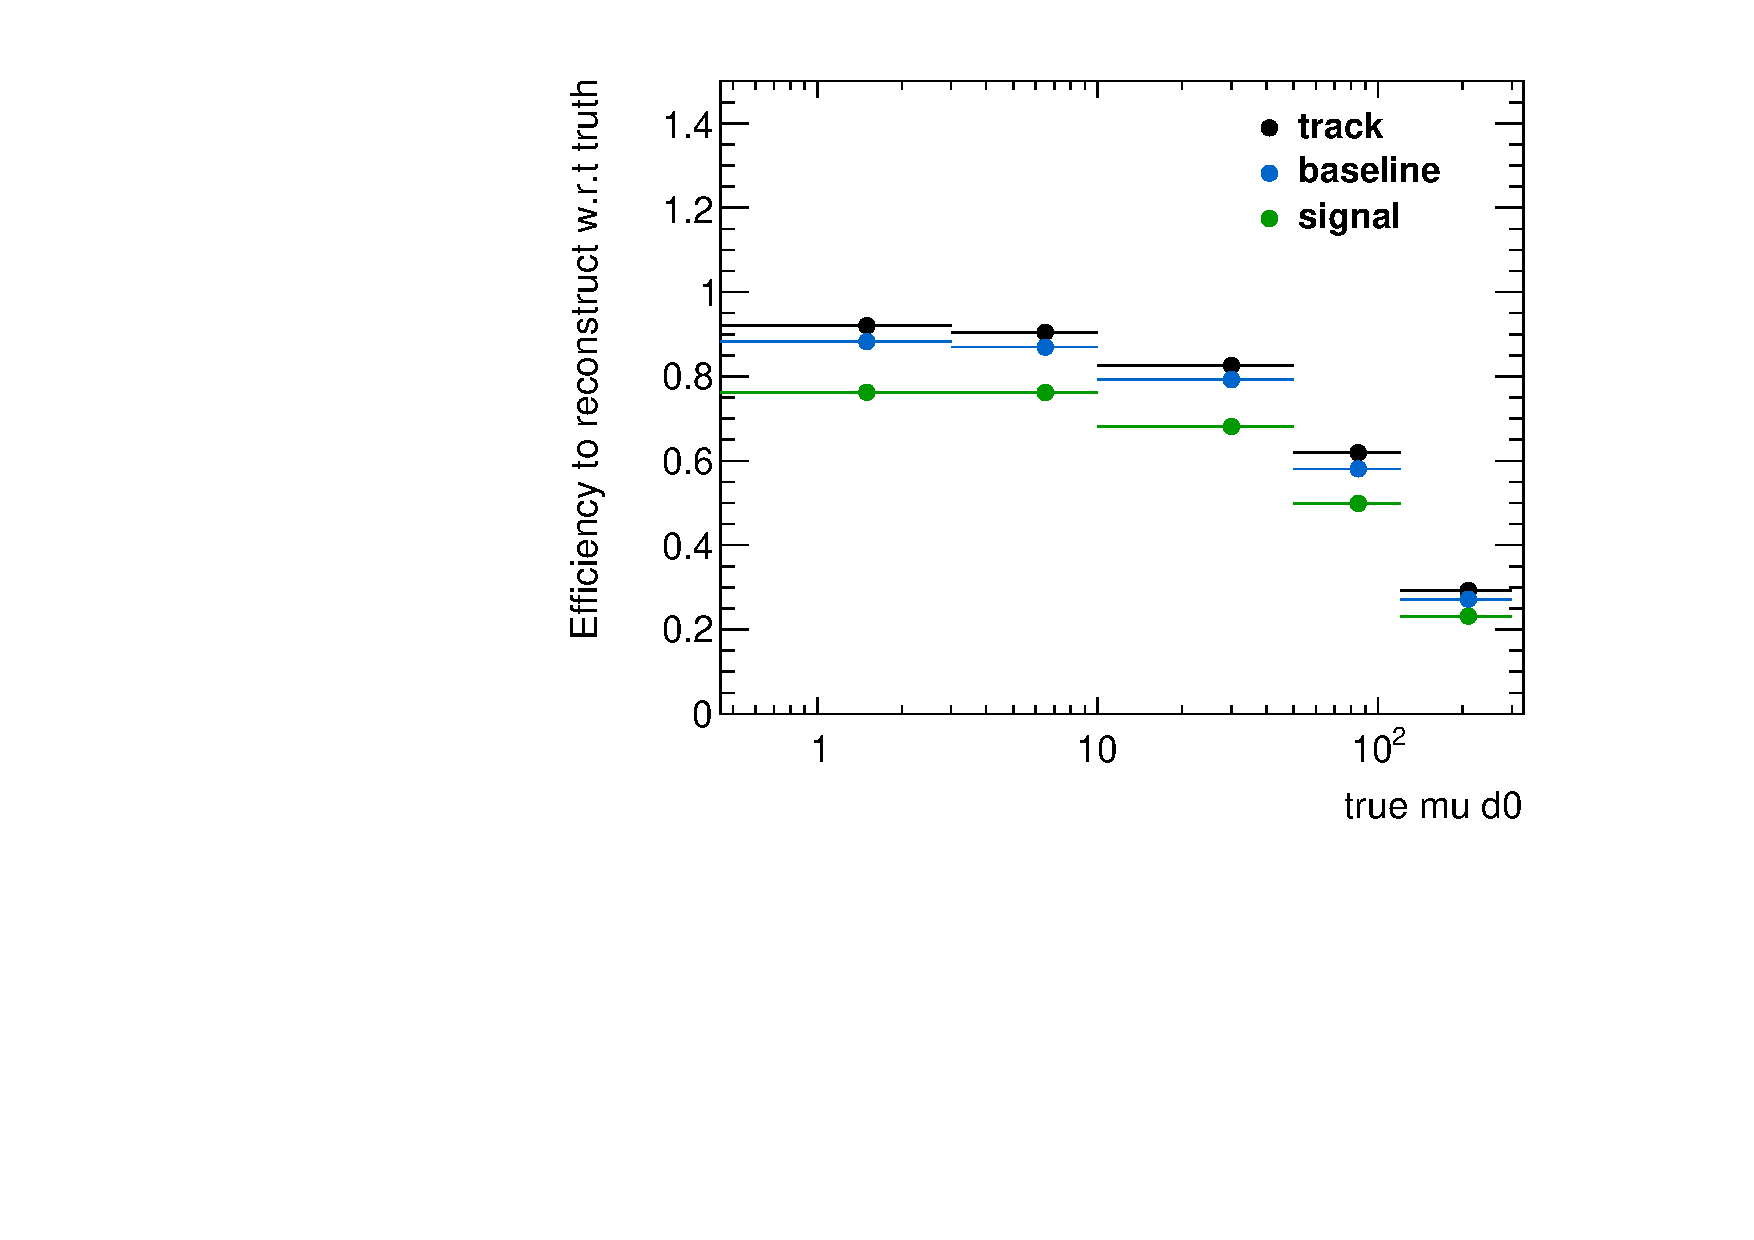
\includegraphics[width=.48\textwidth]{figures/disp_systs/signal_effcompare_d0_mu_300.pdf}
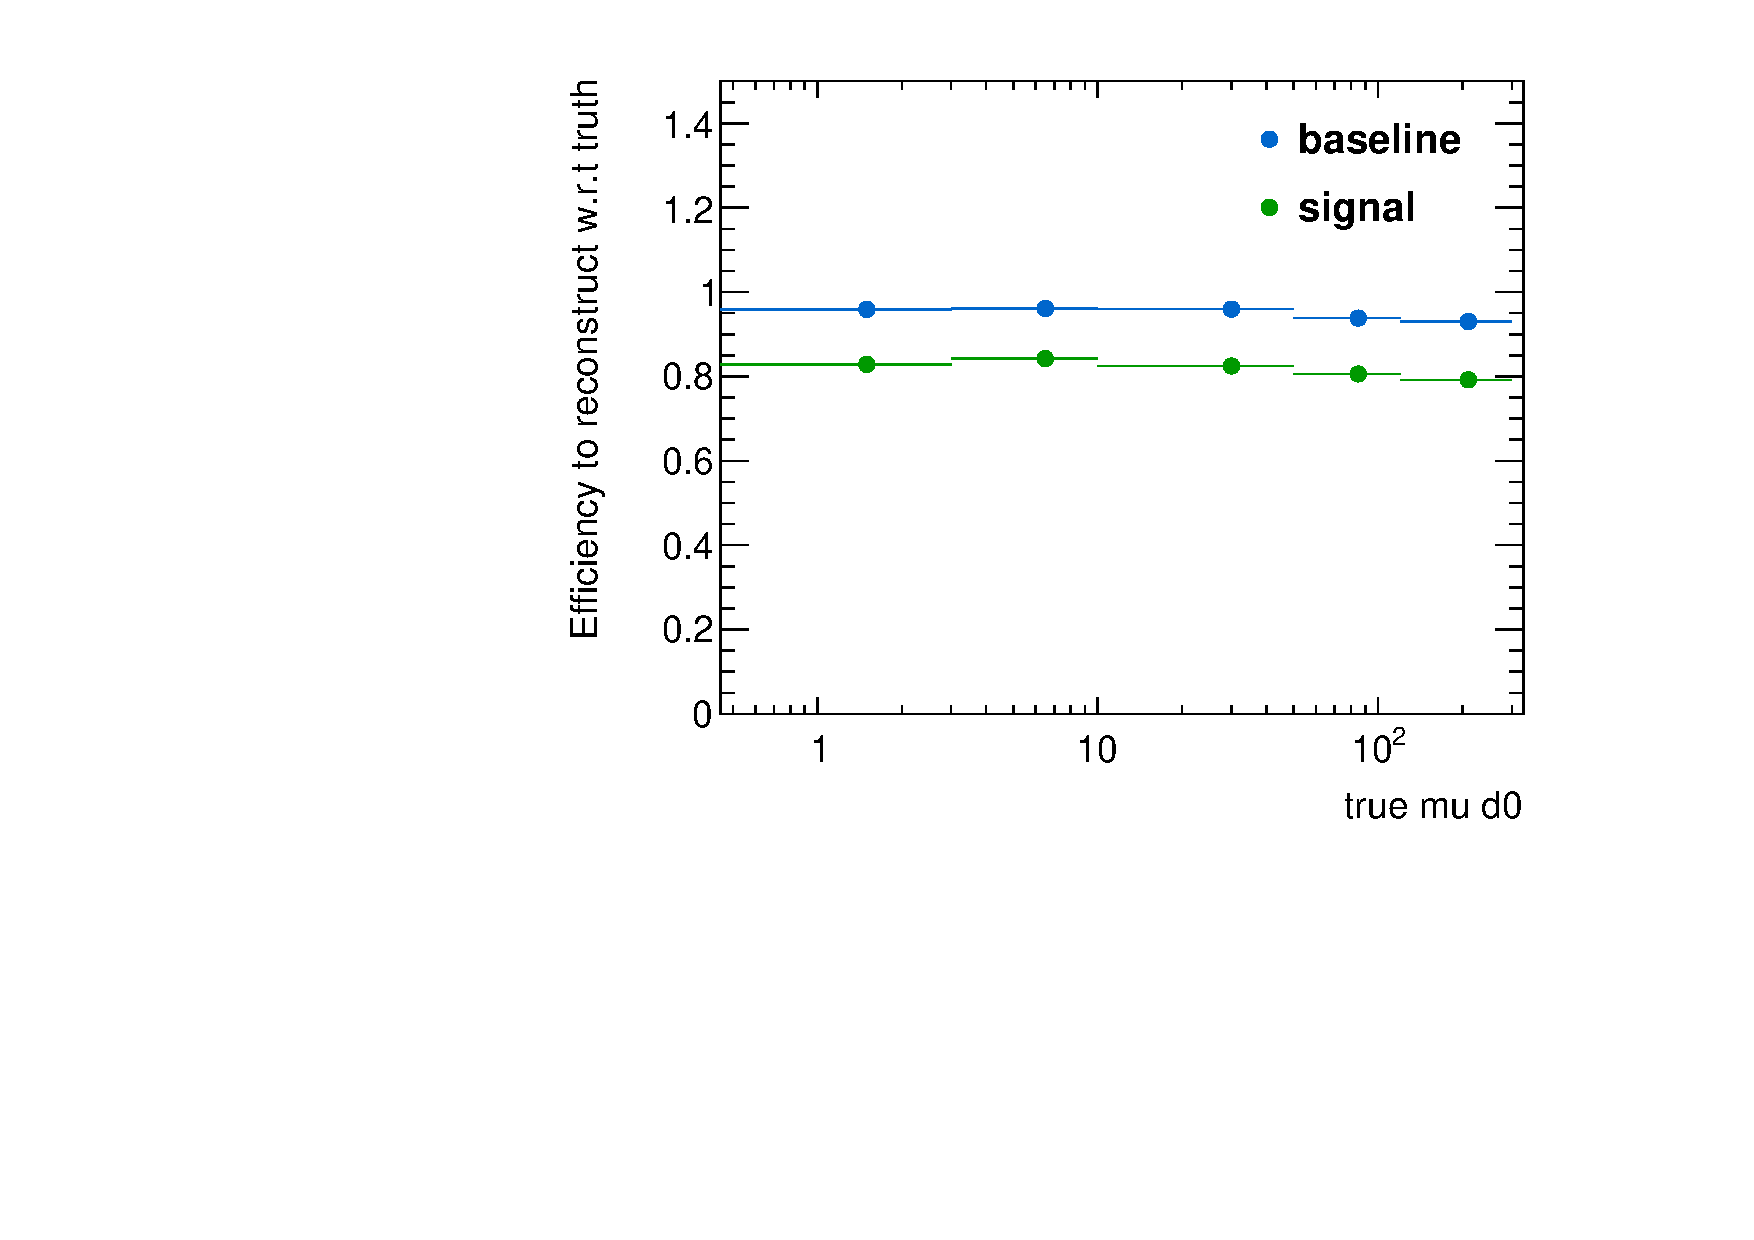
\includegraphics[width=.48\textwidth]{figures/disp_systs/signal_effwrttrack_d0_mu_300.pdf}
\caption{Muon selection efficiencies with respect to truth (left) and with respect to the tracking efficiency (right). Made from a 300 GeV signal sample with lifetimes between 0.01ns-1ns. The denominator of the efficiency is truth muons from sleptons with $\pt > 65 \GeV$ and $|\eta| < 2.5$, and the numerator is truth matched and signal (or baseline) quality tracks or leptons.}
\label{fig:disp_mu}
\end{figure}


%\begin{figure}[htbp]
%\centering
%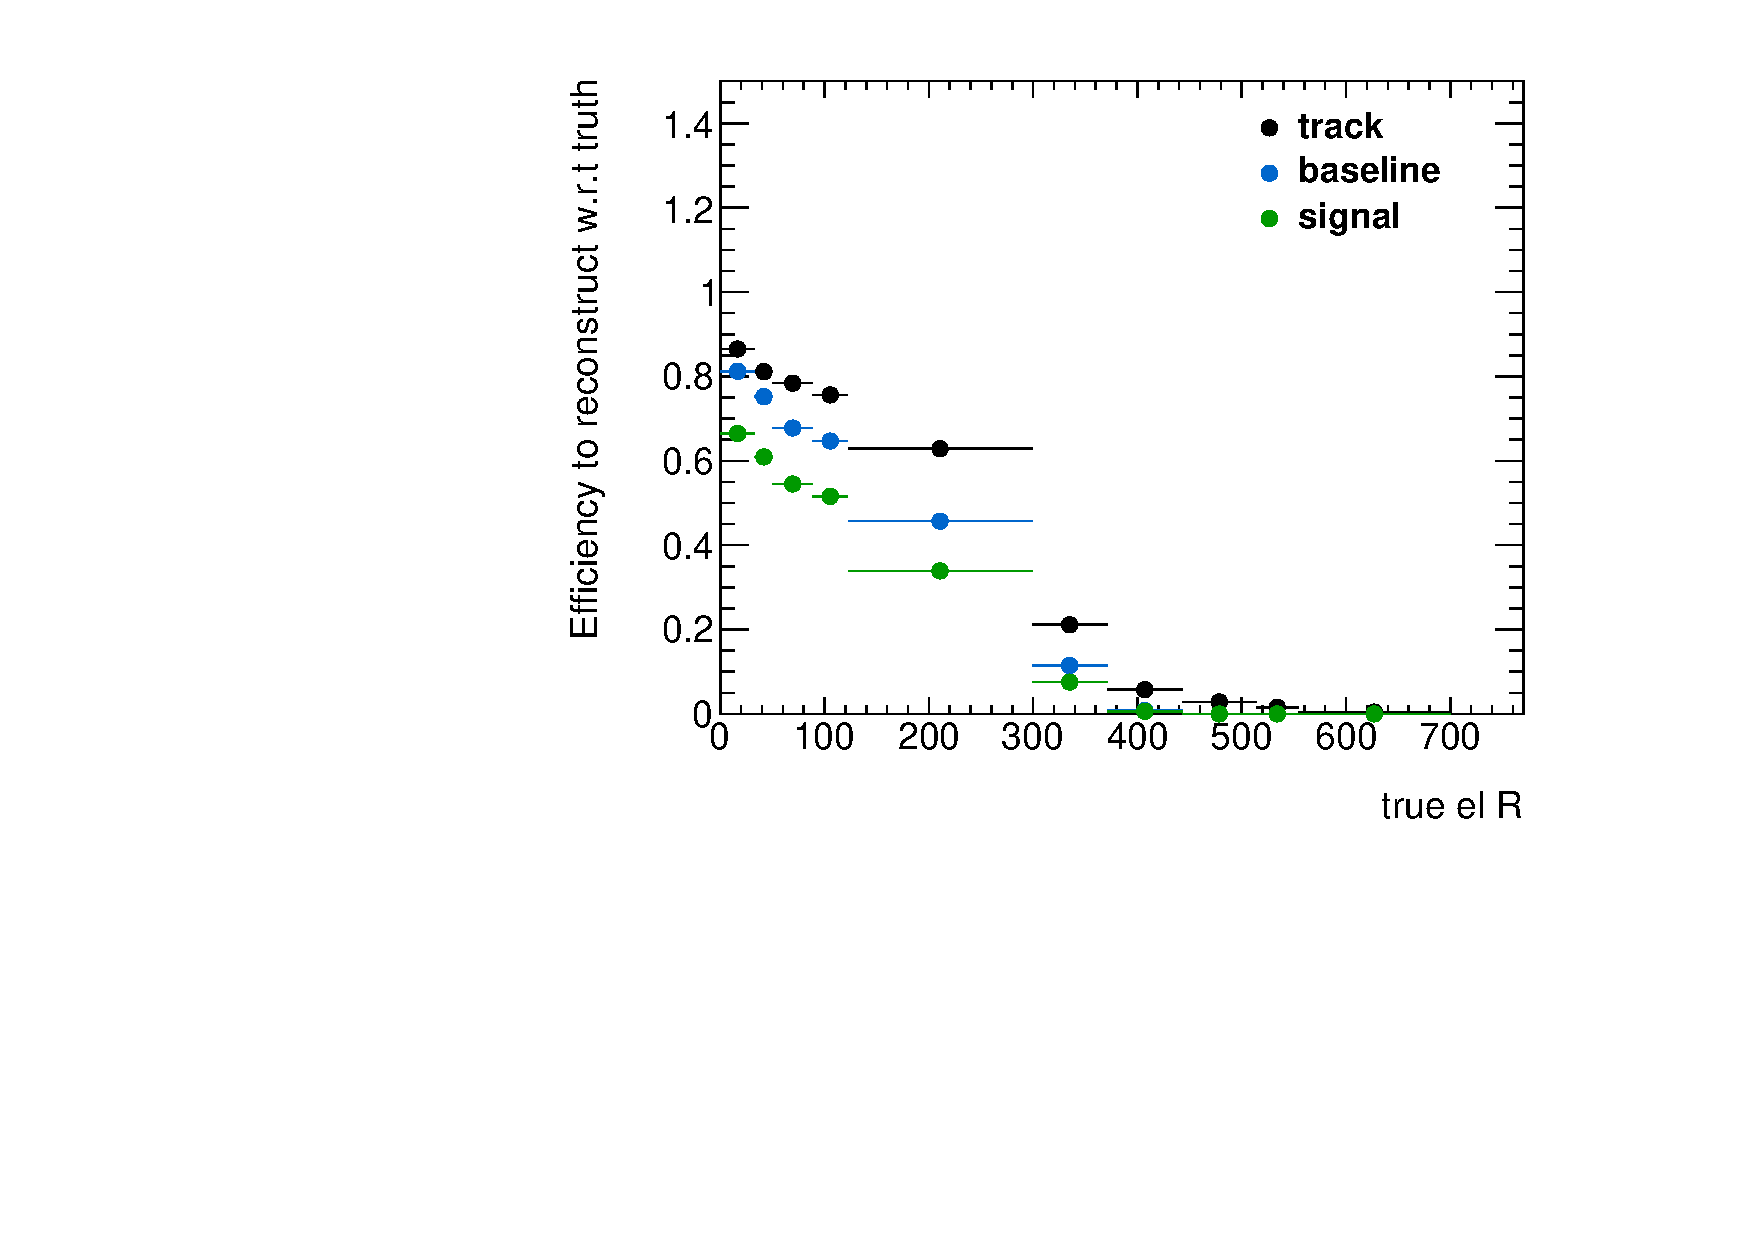
\includegraphics[width=.48\textwidth]{figures/disp_systs/signal_effcompare_R_el_300.pdf}
%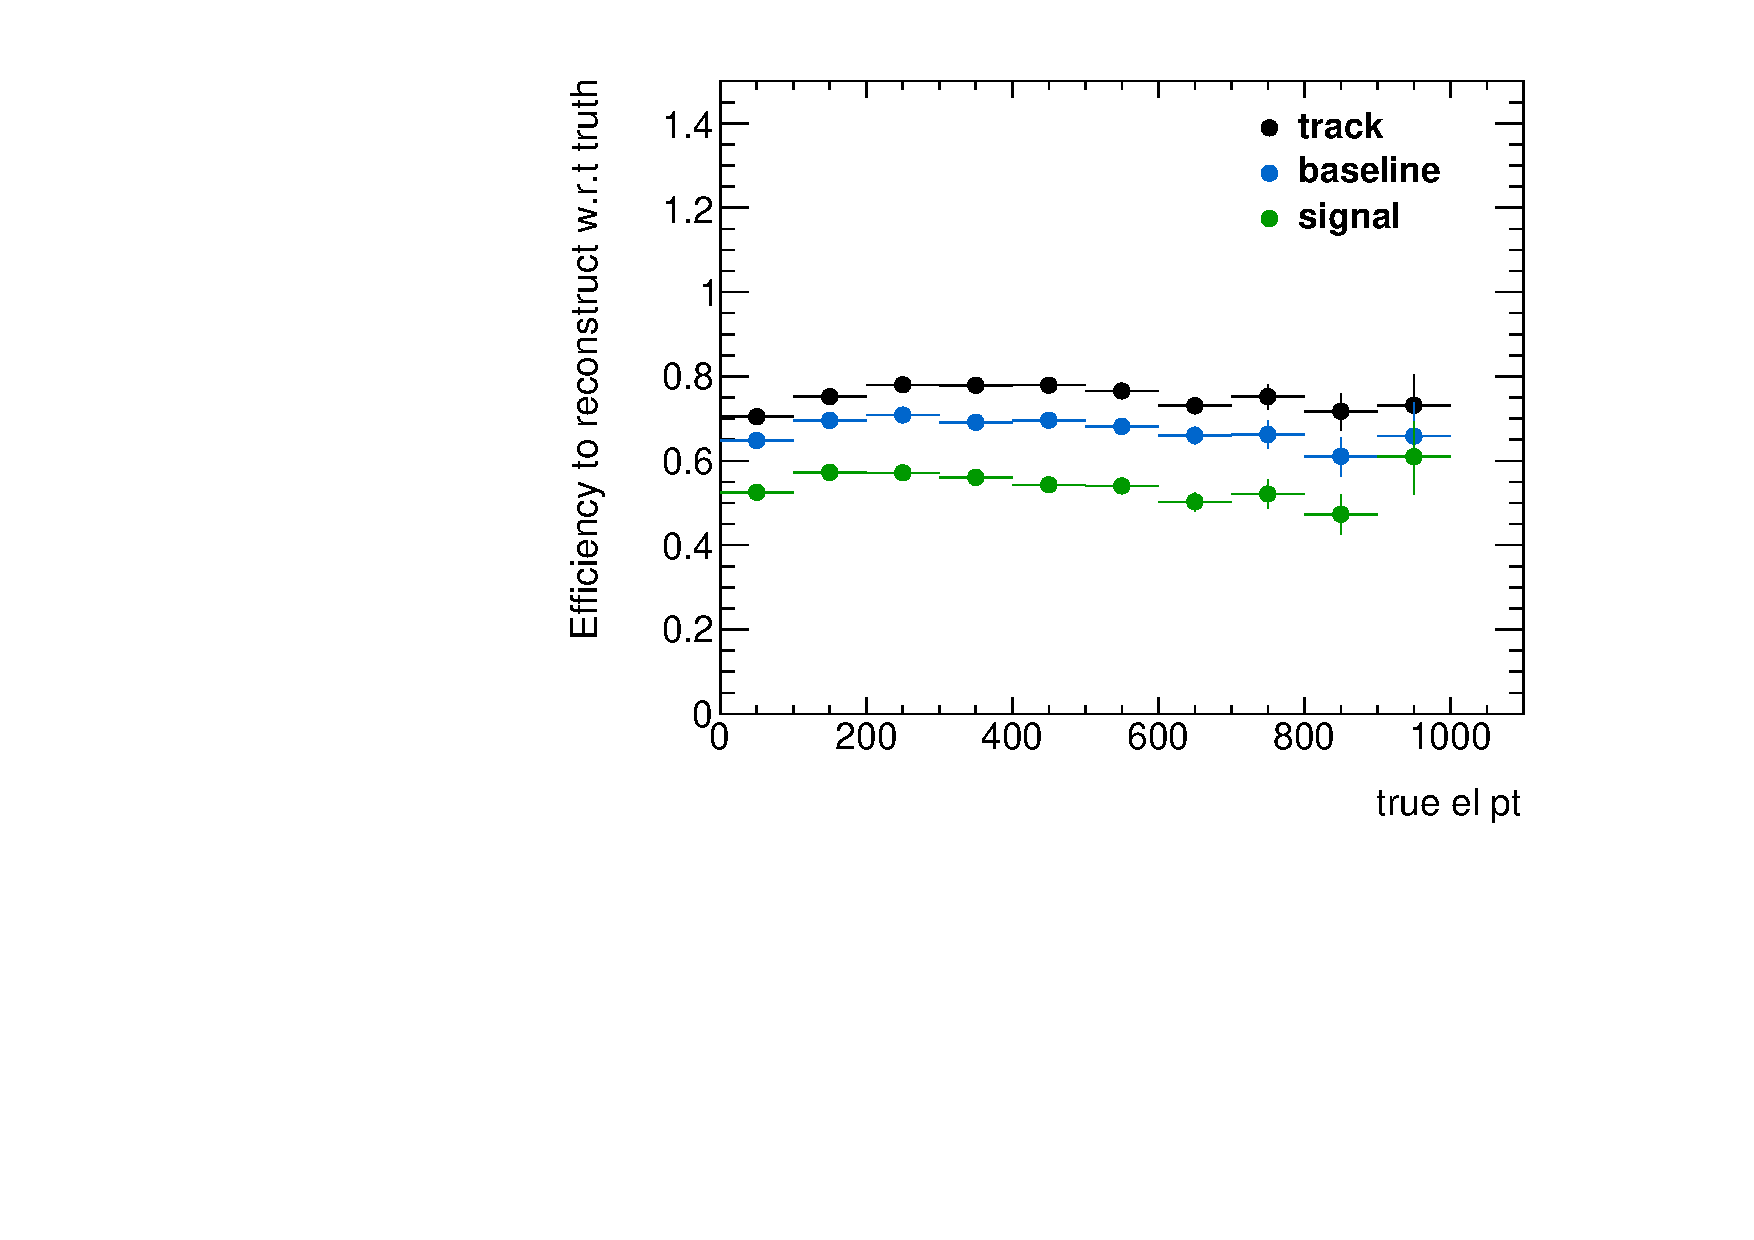
\includegraphics[width=.48\textwidth]{figures/disp_systs/signal_effcompare_pt_el_300.pdf}
%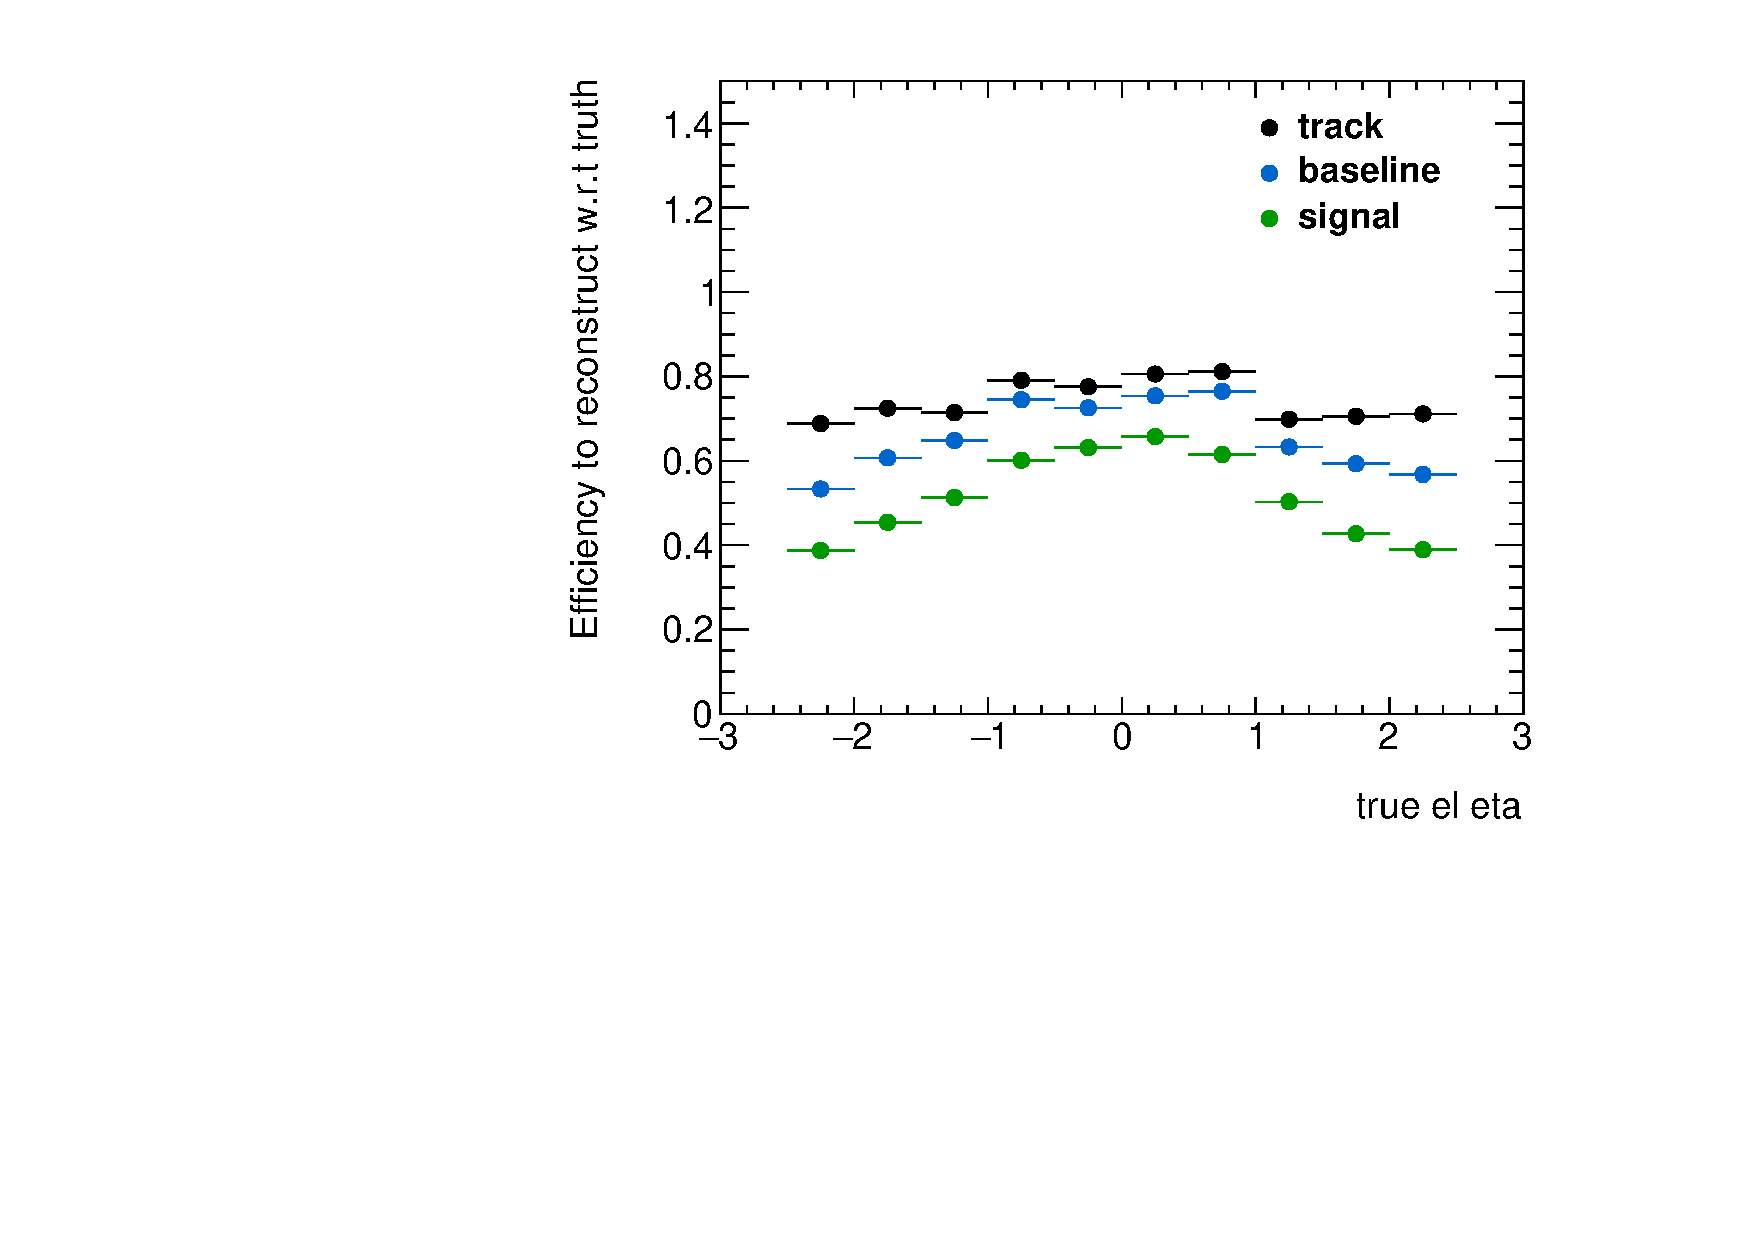
\includegraphics[width=.48\textwidth]{figures/disp_systs/signal_effcompare_eta_el_300.pdf}
%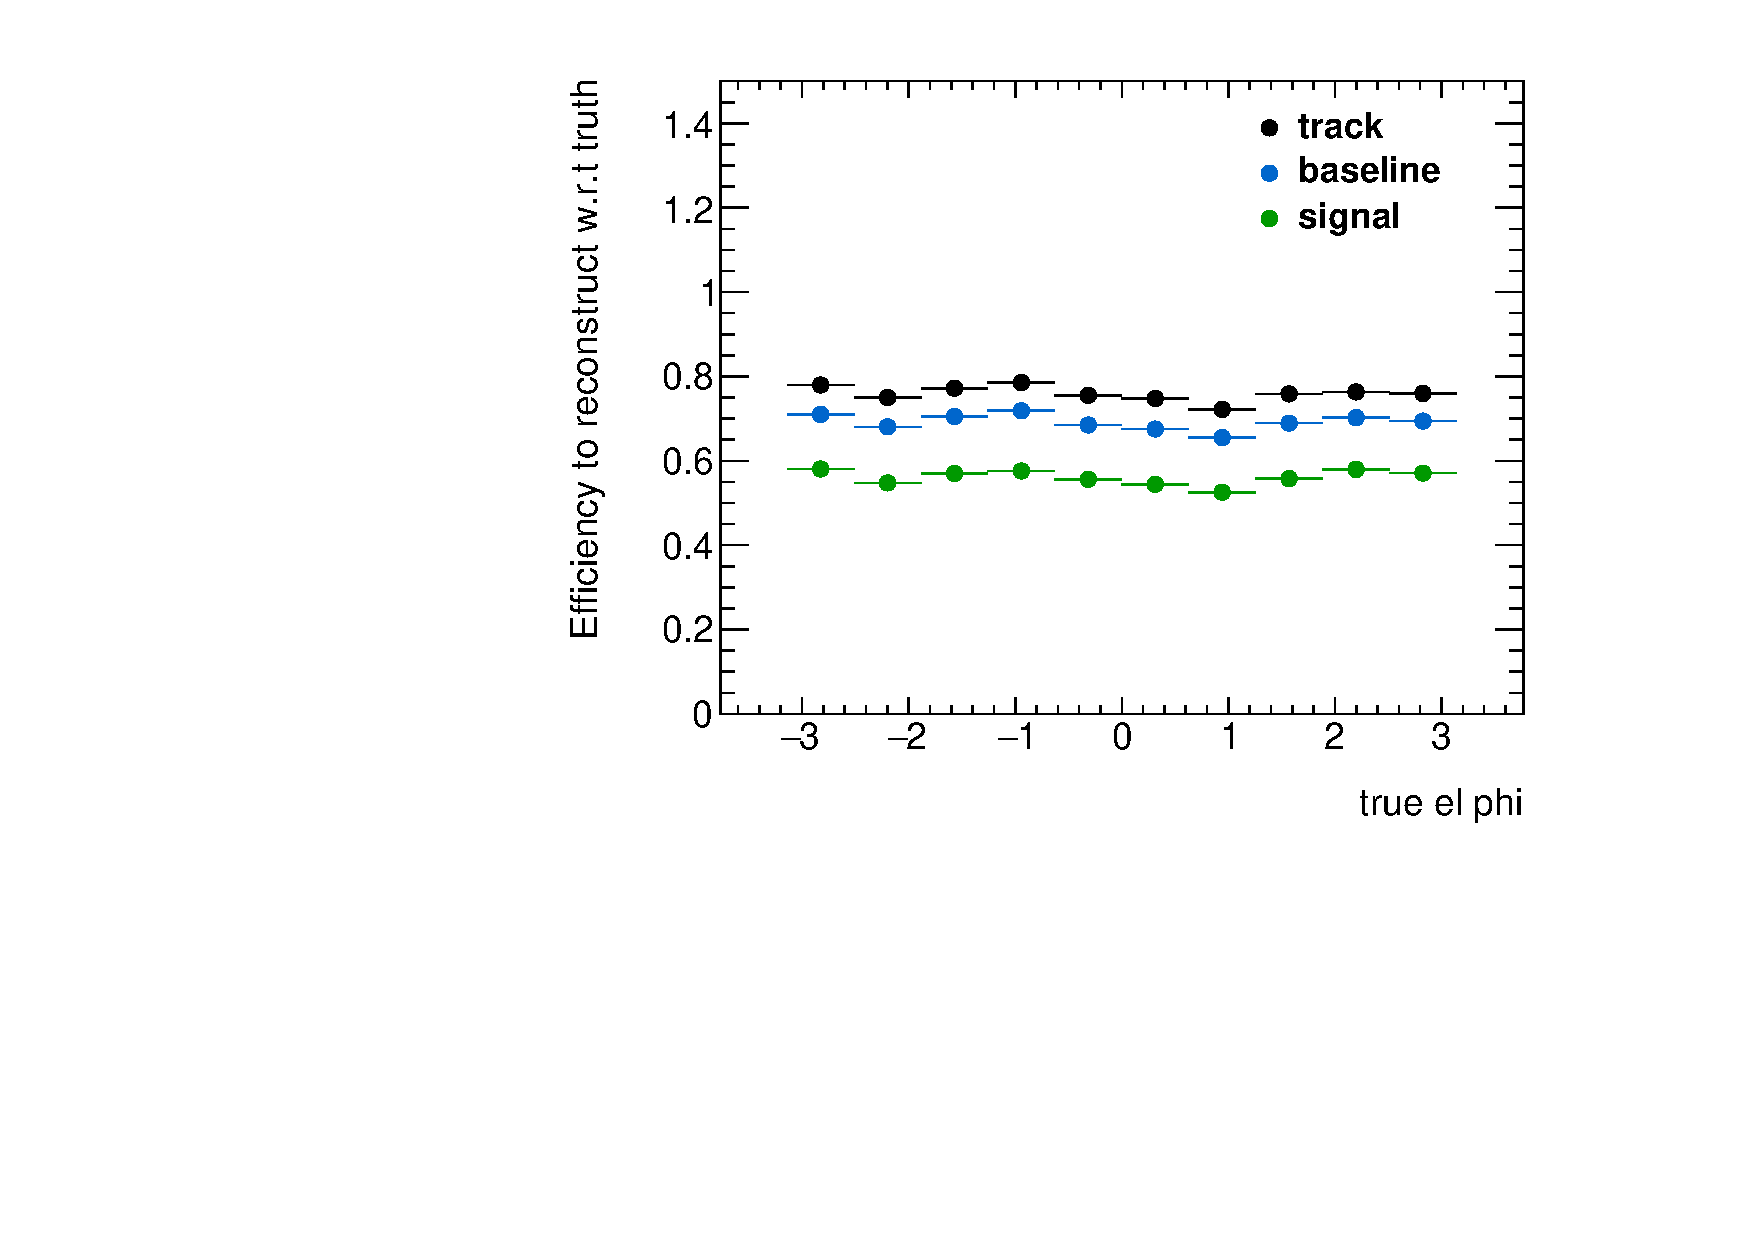
\includegraphics[width=.48\textwidth]{figures/disp_systs/signal_effcompare_phi_el_300.pdf}
%\caption{Electron selection efficiencies vs $R_{\textrm{decay}}$ (top left), \pt (top right), $\eta$ (bottom left), and $\phi$ (bottom right). Plots are made from 300 GeV slepton signal samples with lifetimes between 0.01-1ns. The denominator of the efficiency is truth muons from sleptons with \pt > 65 GeV and $|\eta|$ < 2.5, and the numerator is truth matched and signal (or baseline) quality tracks or leptons.}
%\label{fig:effs_el}
%\end{figure}

%\begin{figure}[htbp]
%\centering
%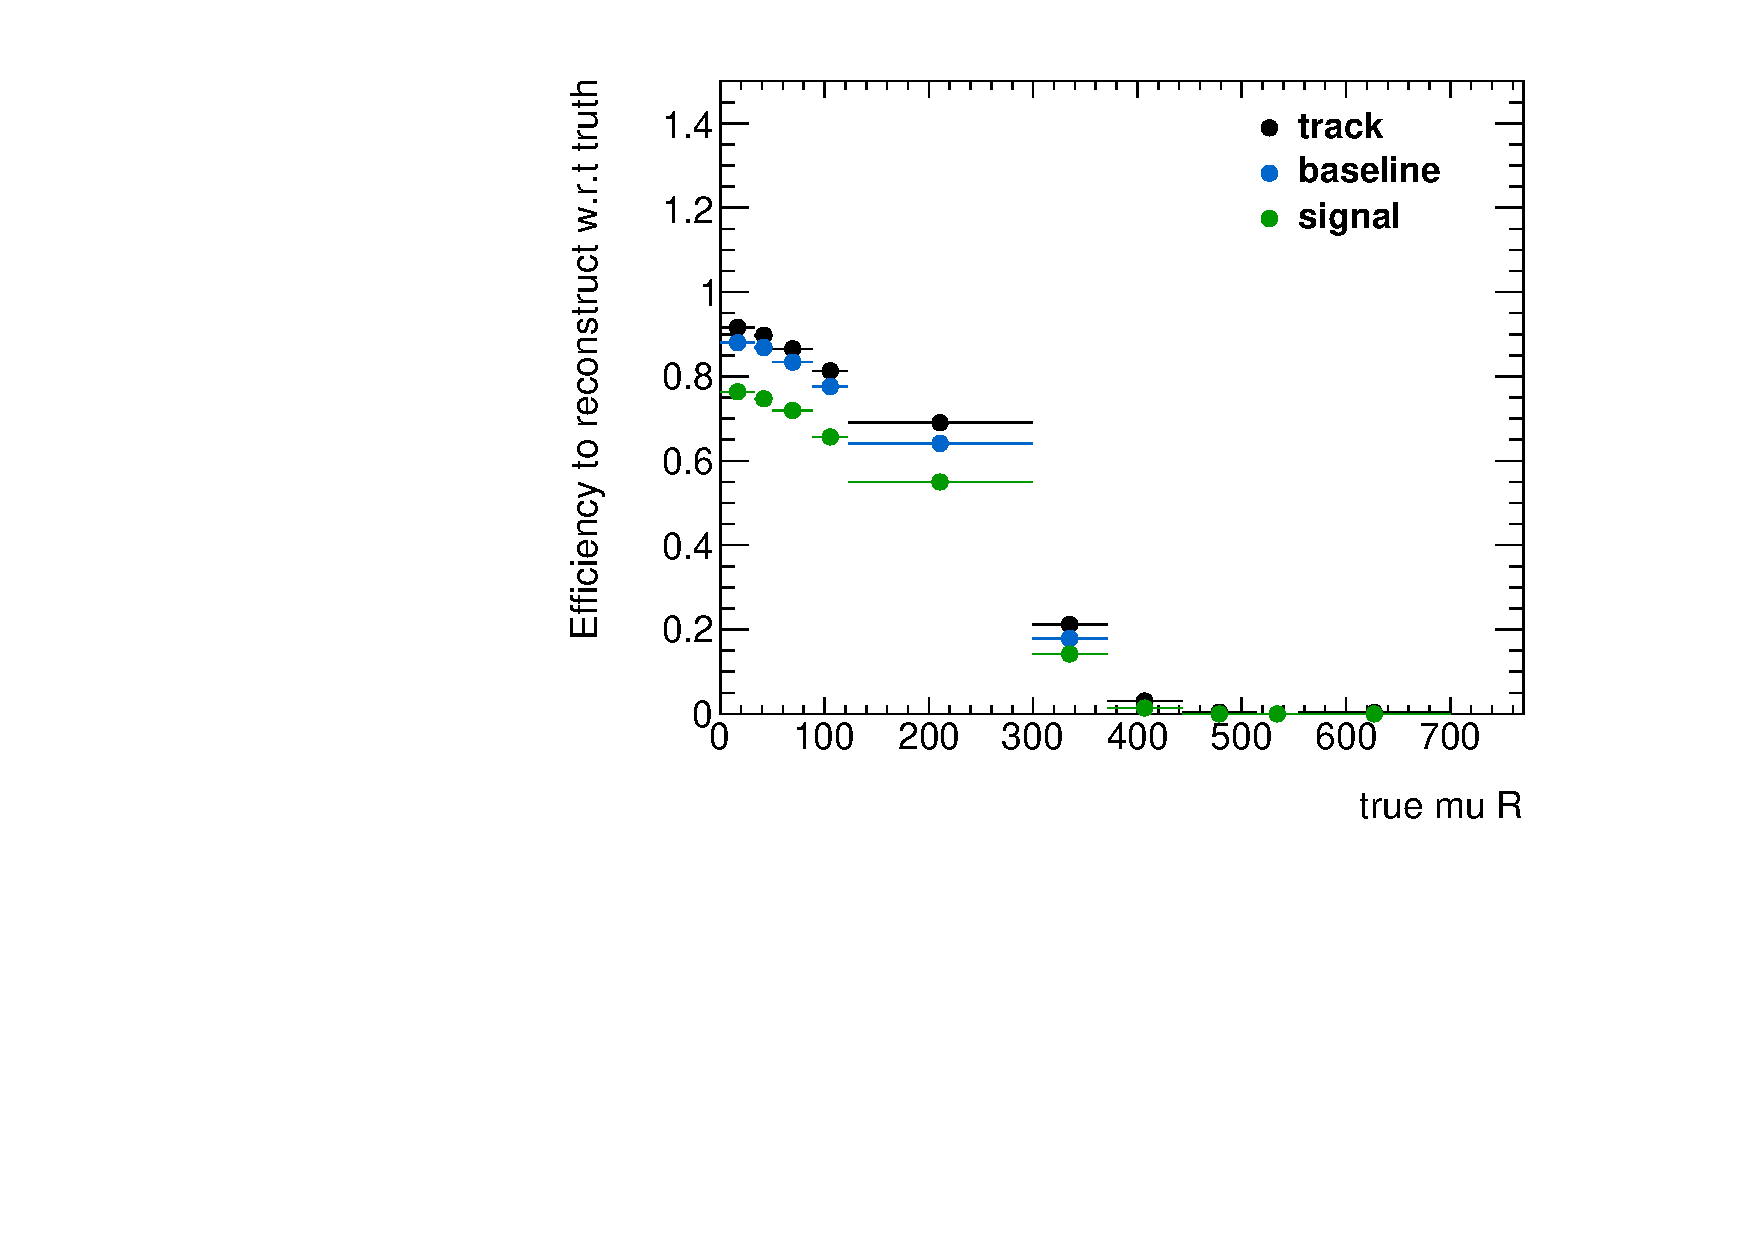
\includegraphics[width=.48\textwidth]{figures/disp_systs/signal_effcompare_R_mu_300.pdf}
%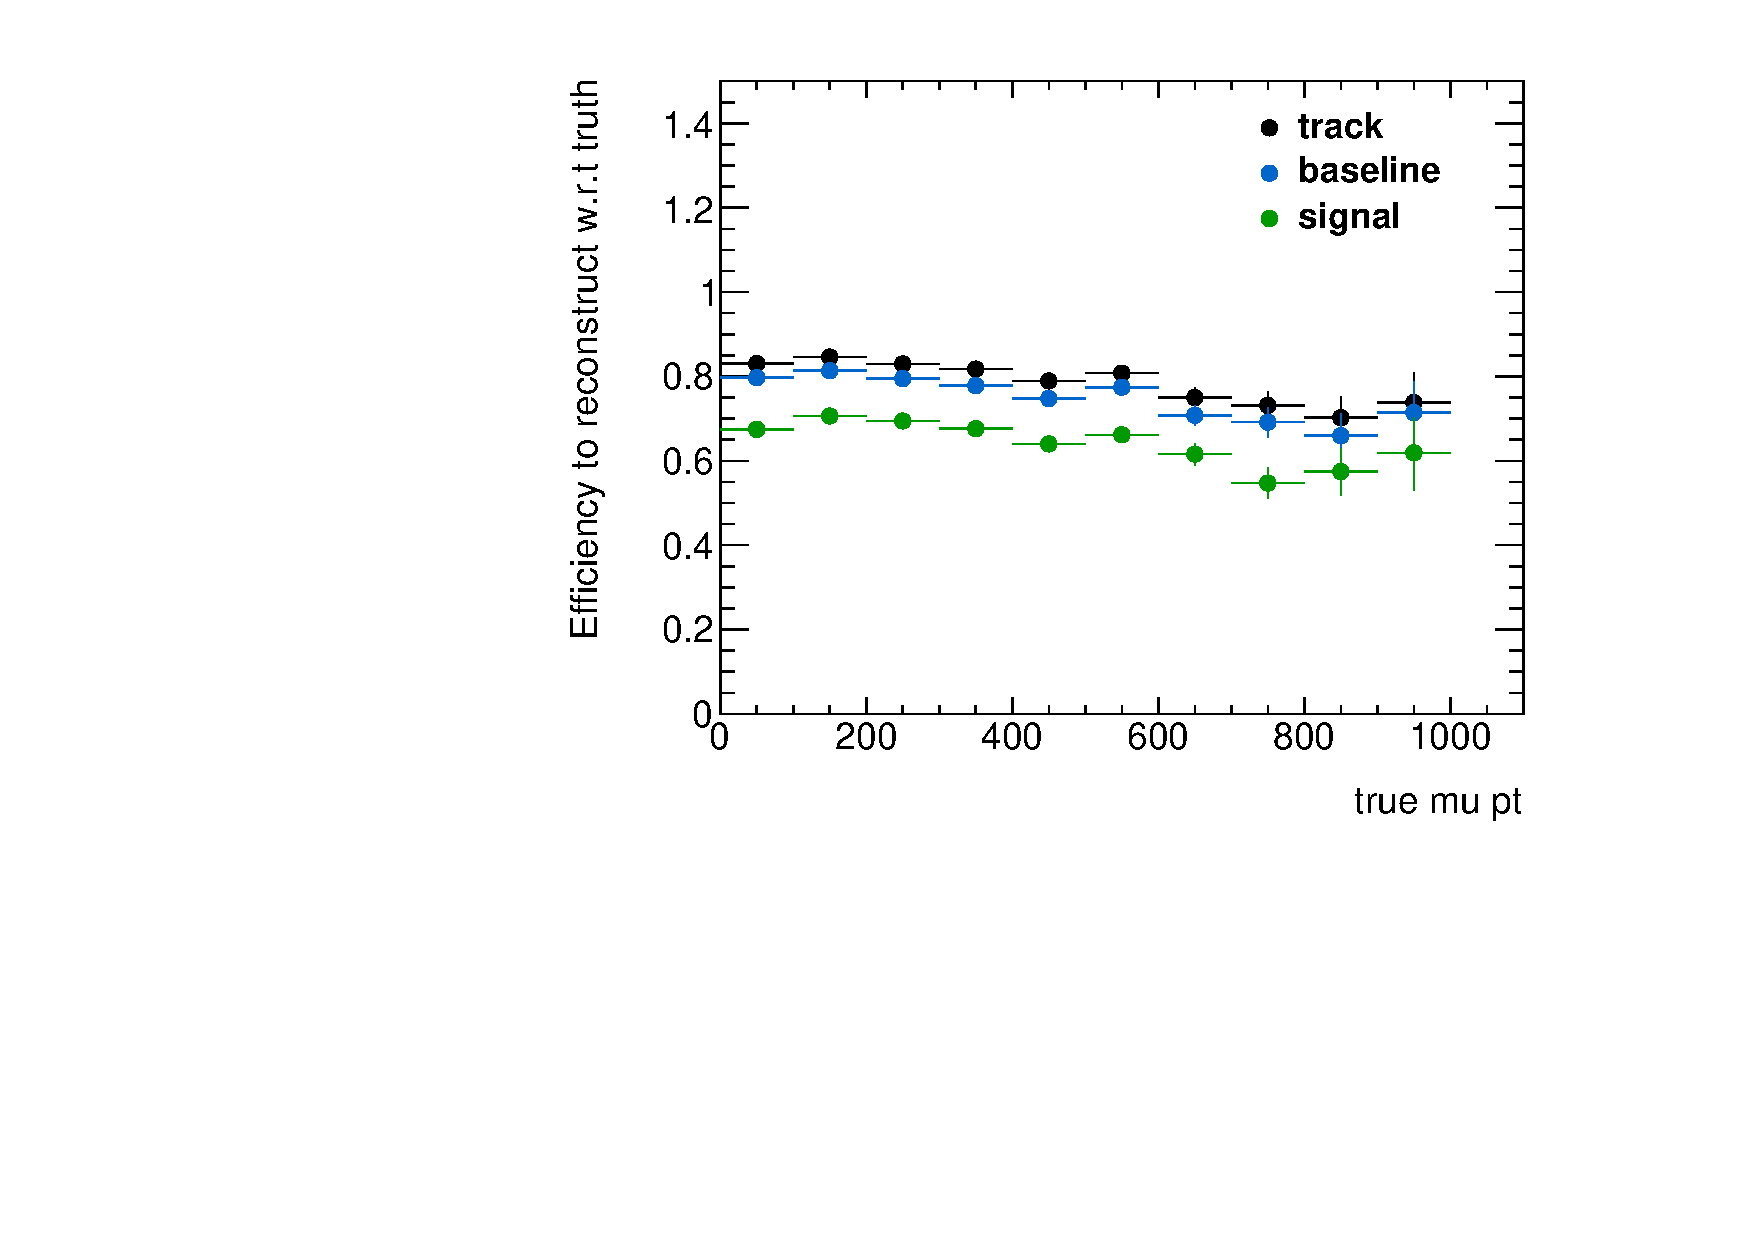
\includegraphics[width=.48\textwidth]{figures/disp_systs/signal_effcompare_pt_mu_300.pdf}
%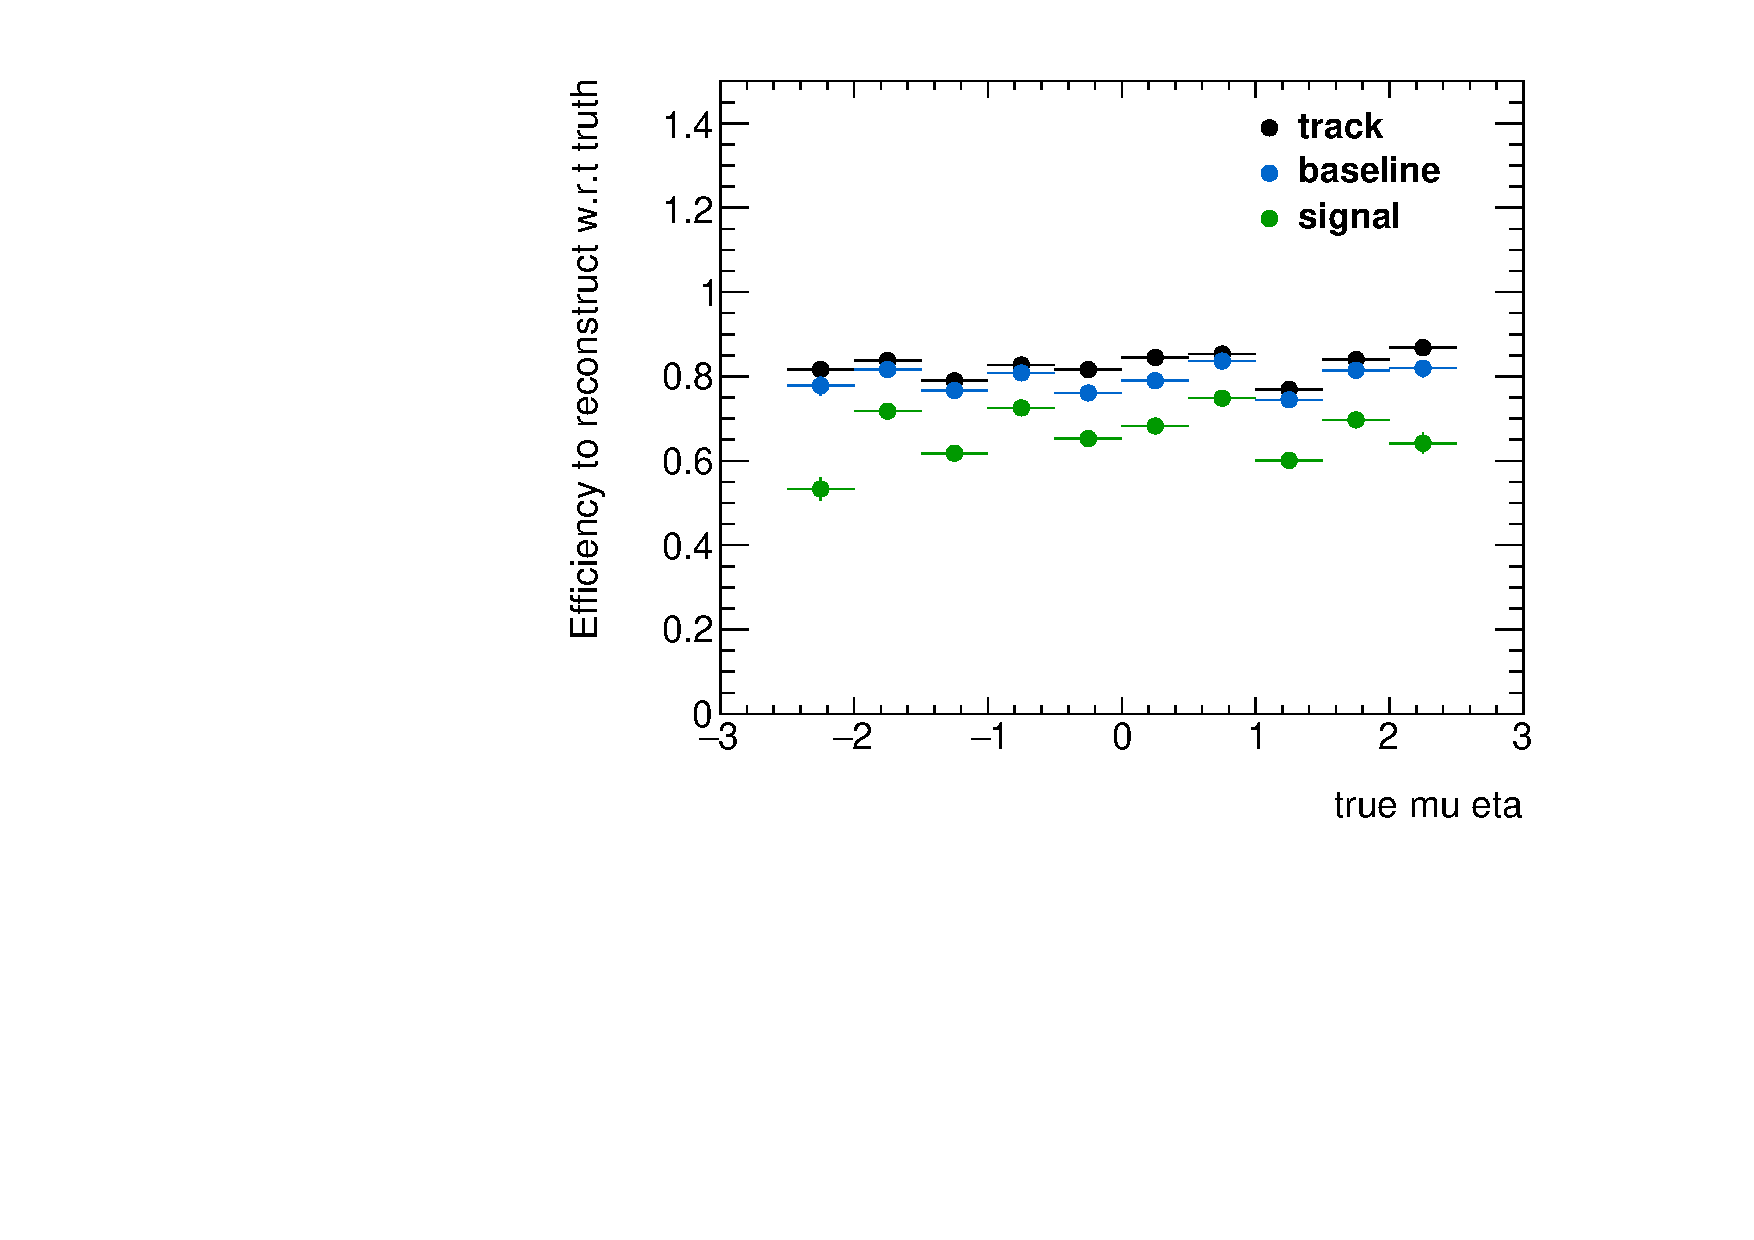
\includegraphics[width=.48\textwidth]{figures/disp_systs/signal_effcompare_eta_mu_300.pdf}
%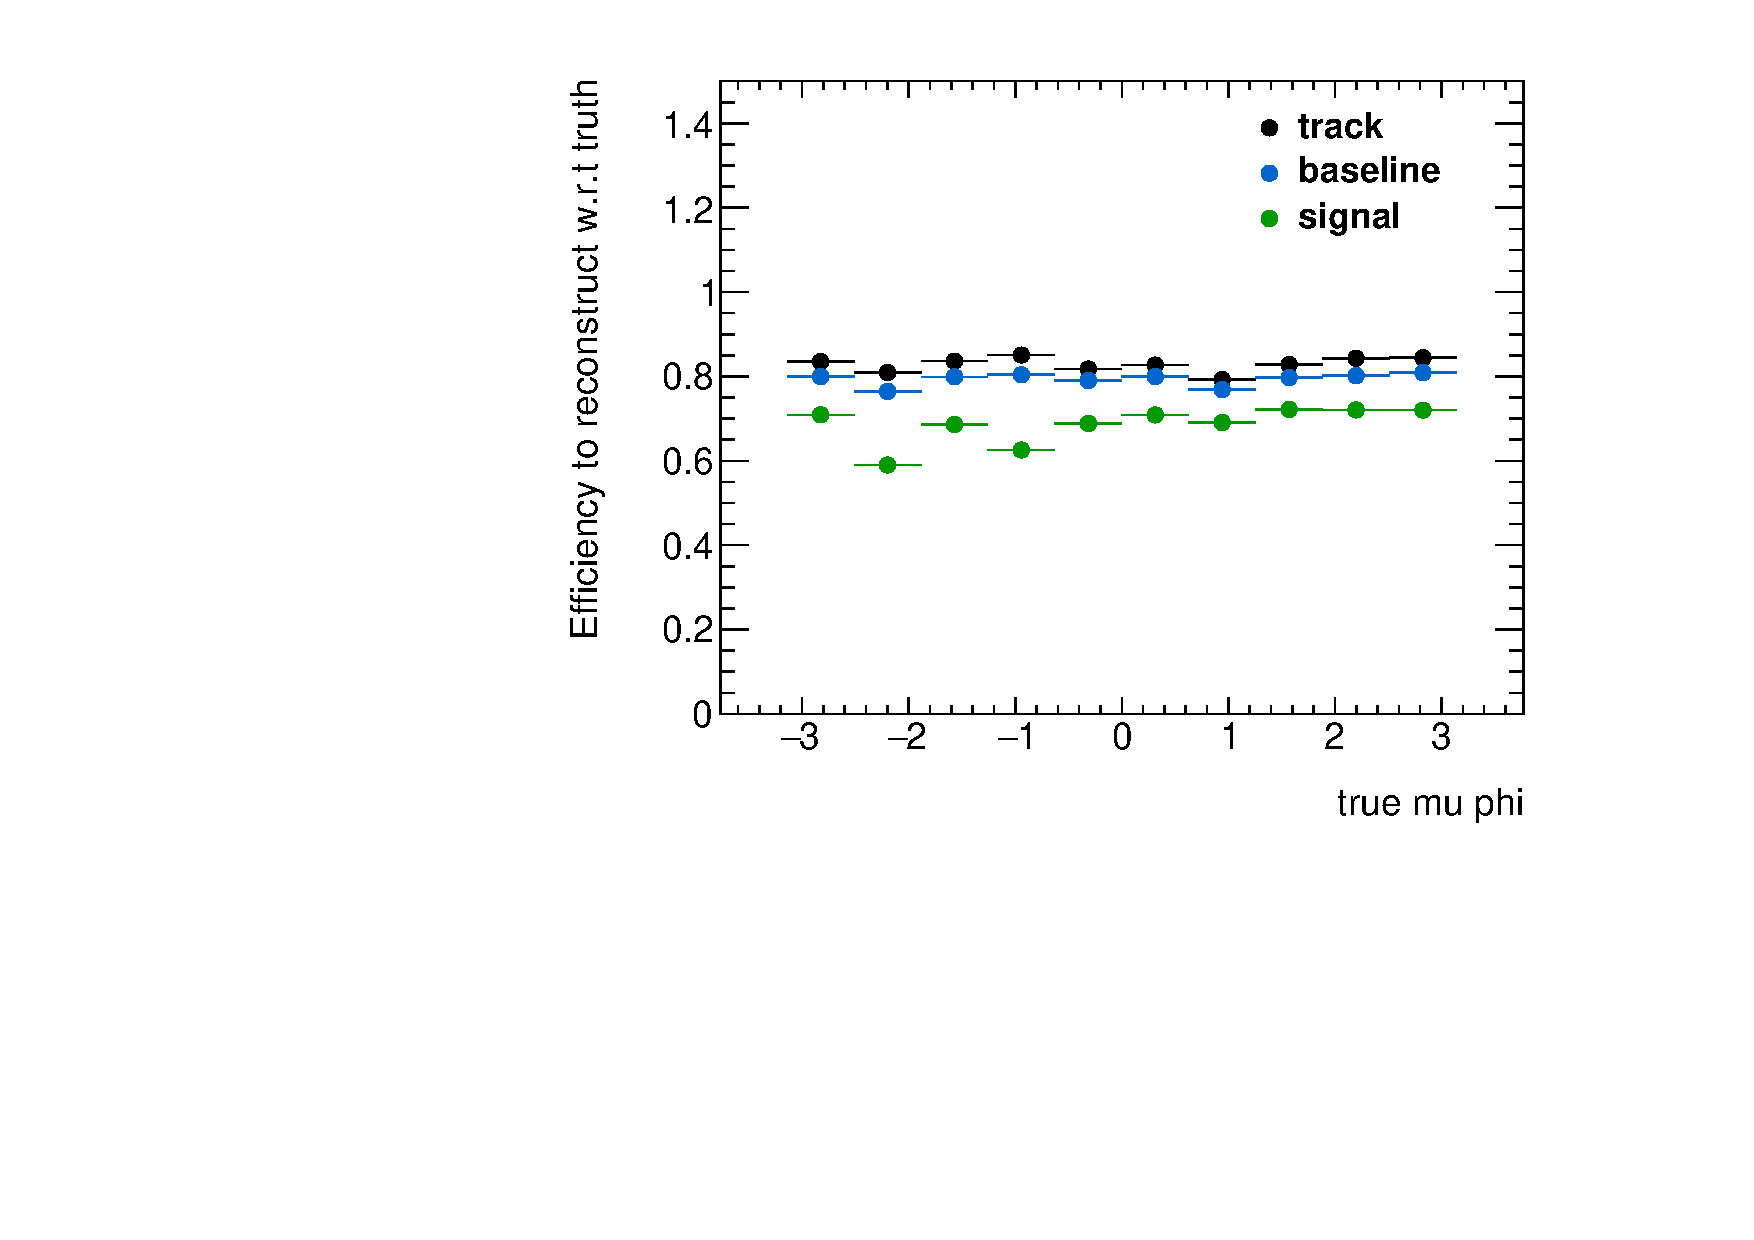
\includegraphics[width=.48\textwidth]{figures/disp_systs/signal_effcompare_phi_mu_300.pdf}
%\caption{Electron selection efficiencies vs $R_{\textrm{decay}}$ (top left), \pt (top right), $\eta$ (bottom left), and $\phi$ (bottom right). Plots are made from 300 GeV slepton signal samples with lifetimes between 0.01-1ns. The denominator of the efficiency is truth muons from sleptons with \pt > 65 GeV and $|\eta|$ < 2.5, and the numerator is truth matched and signal (or baseline) quality tracks or leptons.}
%\label{fig:effs_mu}
%\end{figure}



Small trends in \dz can be seen in some shower shape variables, particularly in ERatio and RHad, though not enough to explain the full discrepancy. In muons, trends can be seen in the \ac{MS} track $\chi^{2}$ as well as the Eloss, and in electrons trends can be seen in $f_{1}$ and ERatio. We checked for, but did not find, trends in \dz with respect to other \ac{MS} track or shower shape variables. 


\begin{figure}[htbp]
\centering
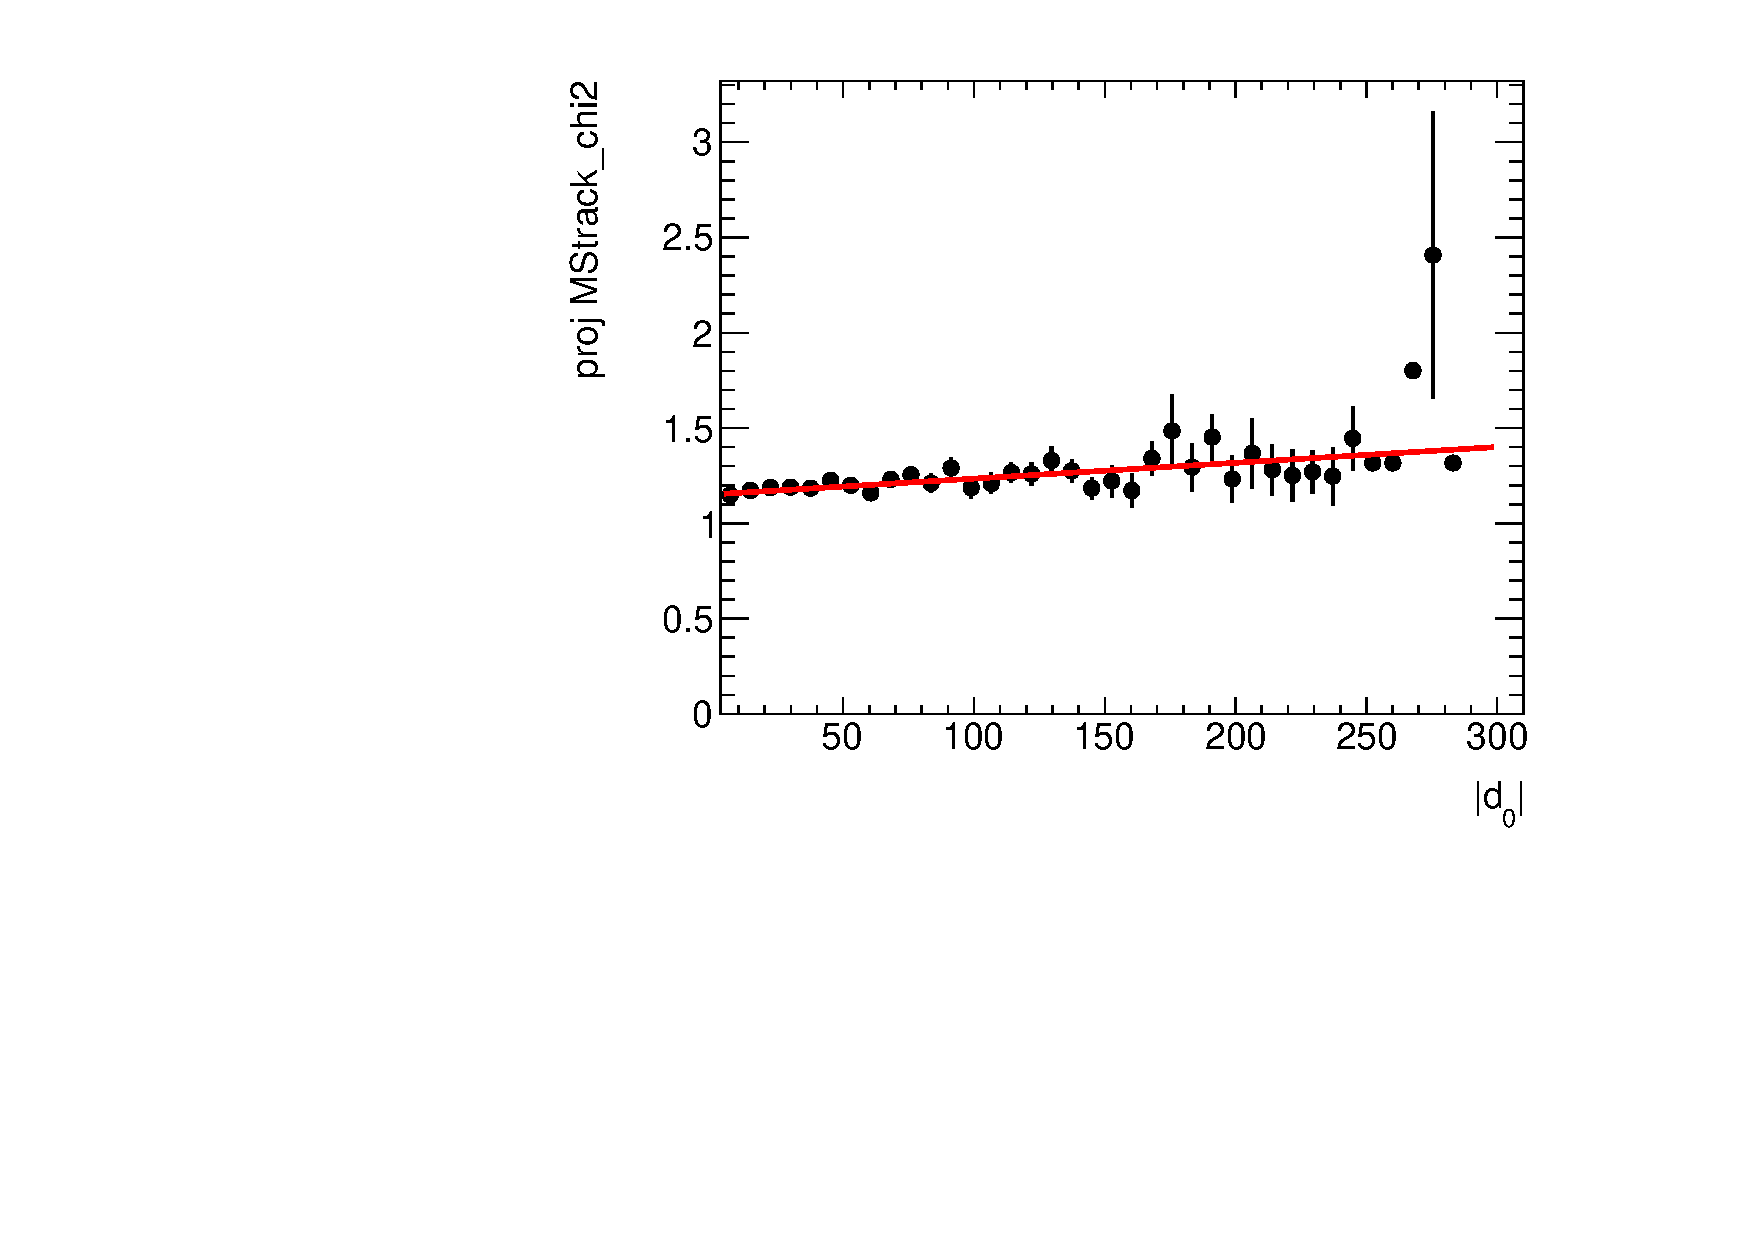
\includegraphics[width=.48\textwidth]{figures/disp_systs/m_signal_MStrack_chi2_profile.pdf}
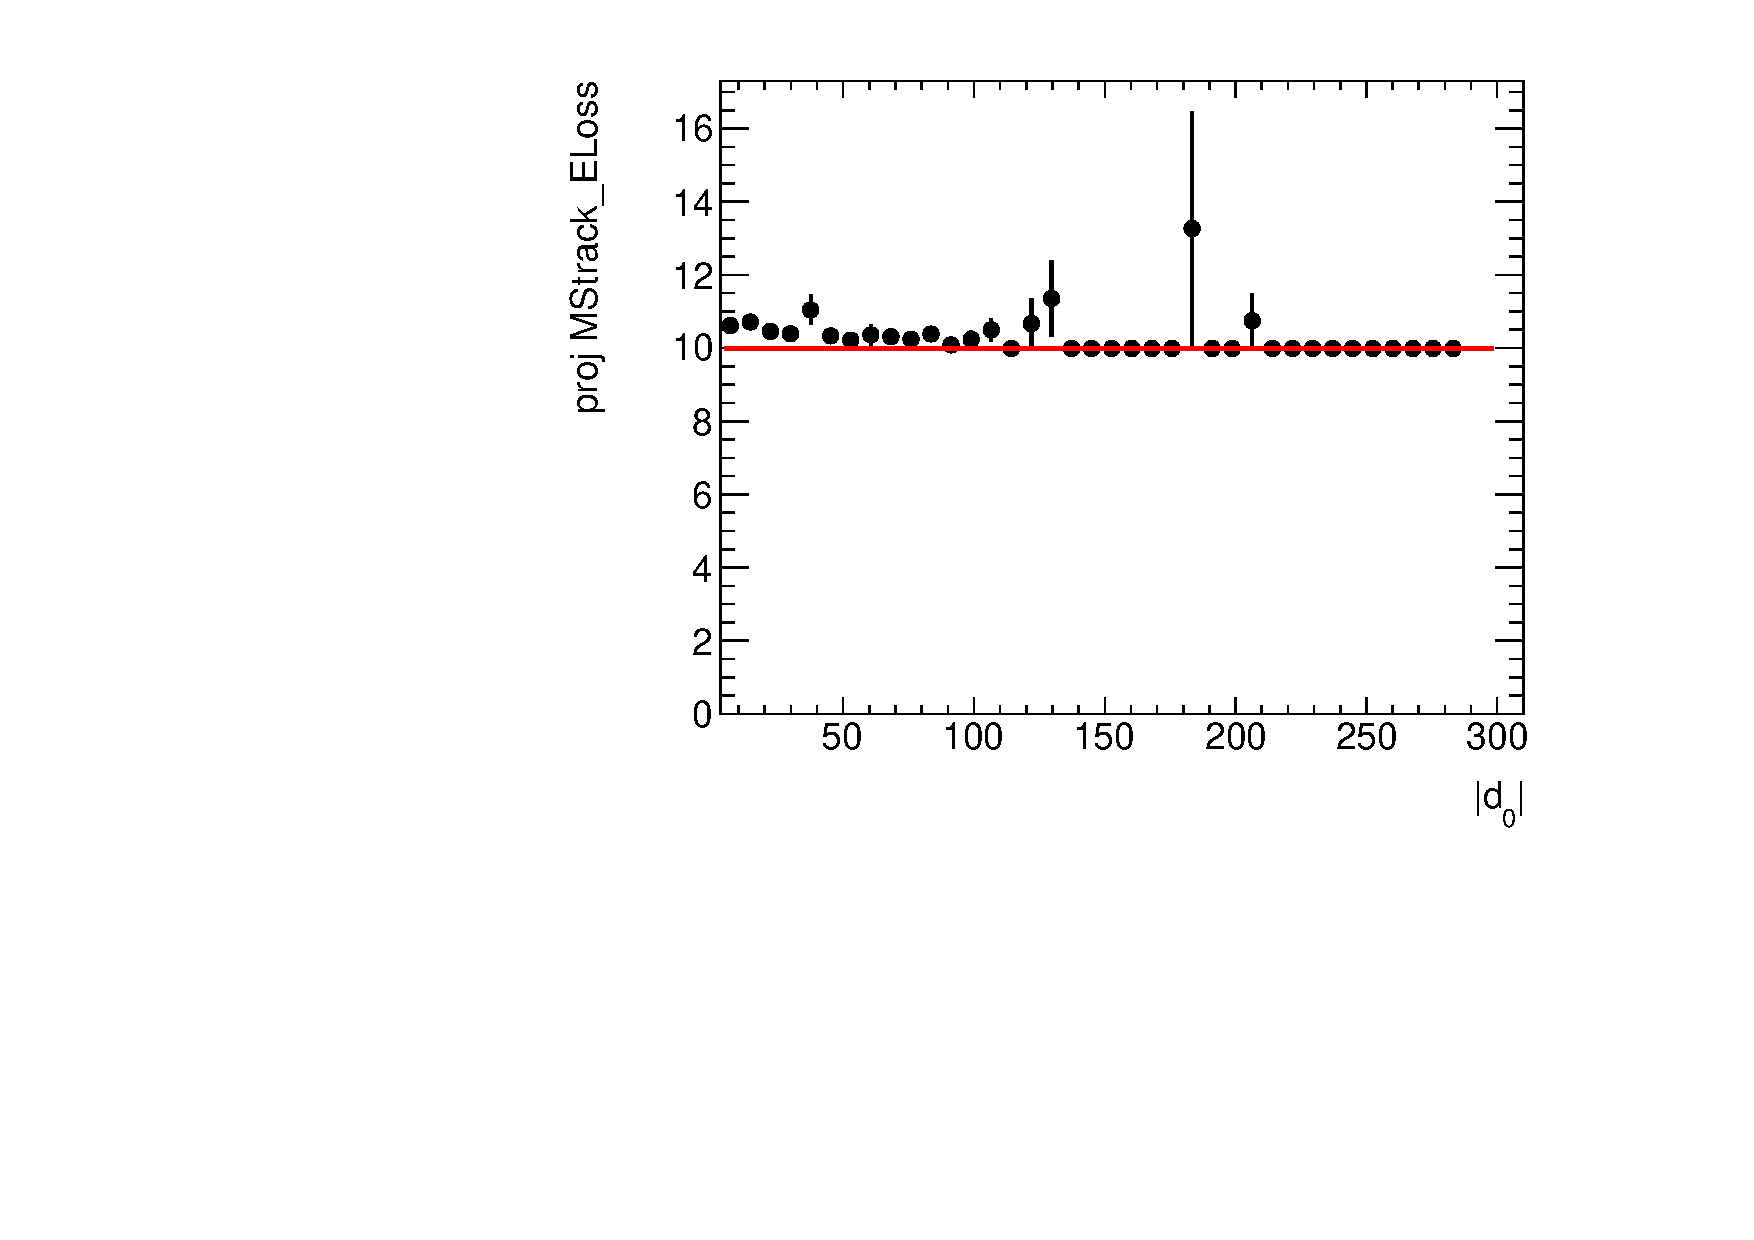
\includegraphics[width=.48\textwidth]{figures/disp_systs/m_signal_MStrack_ELoss_profile.pdf}
\caption{Muon quality variables with trends with respect to \absdz, \ac{MS} track $\chi^{2}$ (left) and Eloss. Taken from a 300 GeV signal sample with lifetimes between 0.01ns-1ns.}
\label{fig:profs_mu}
\end{figure}

\begin{figure}[htbp]
\centering
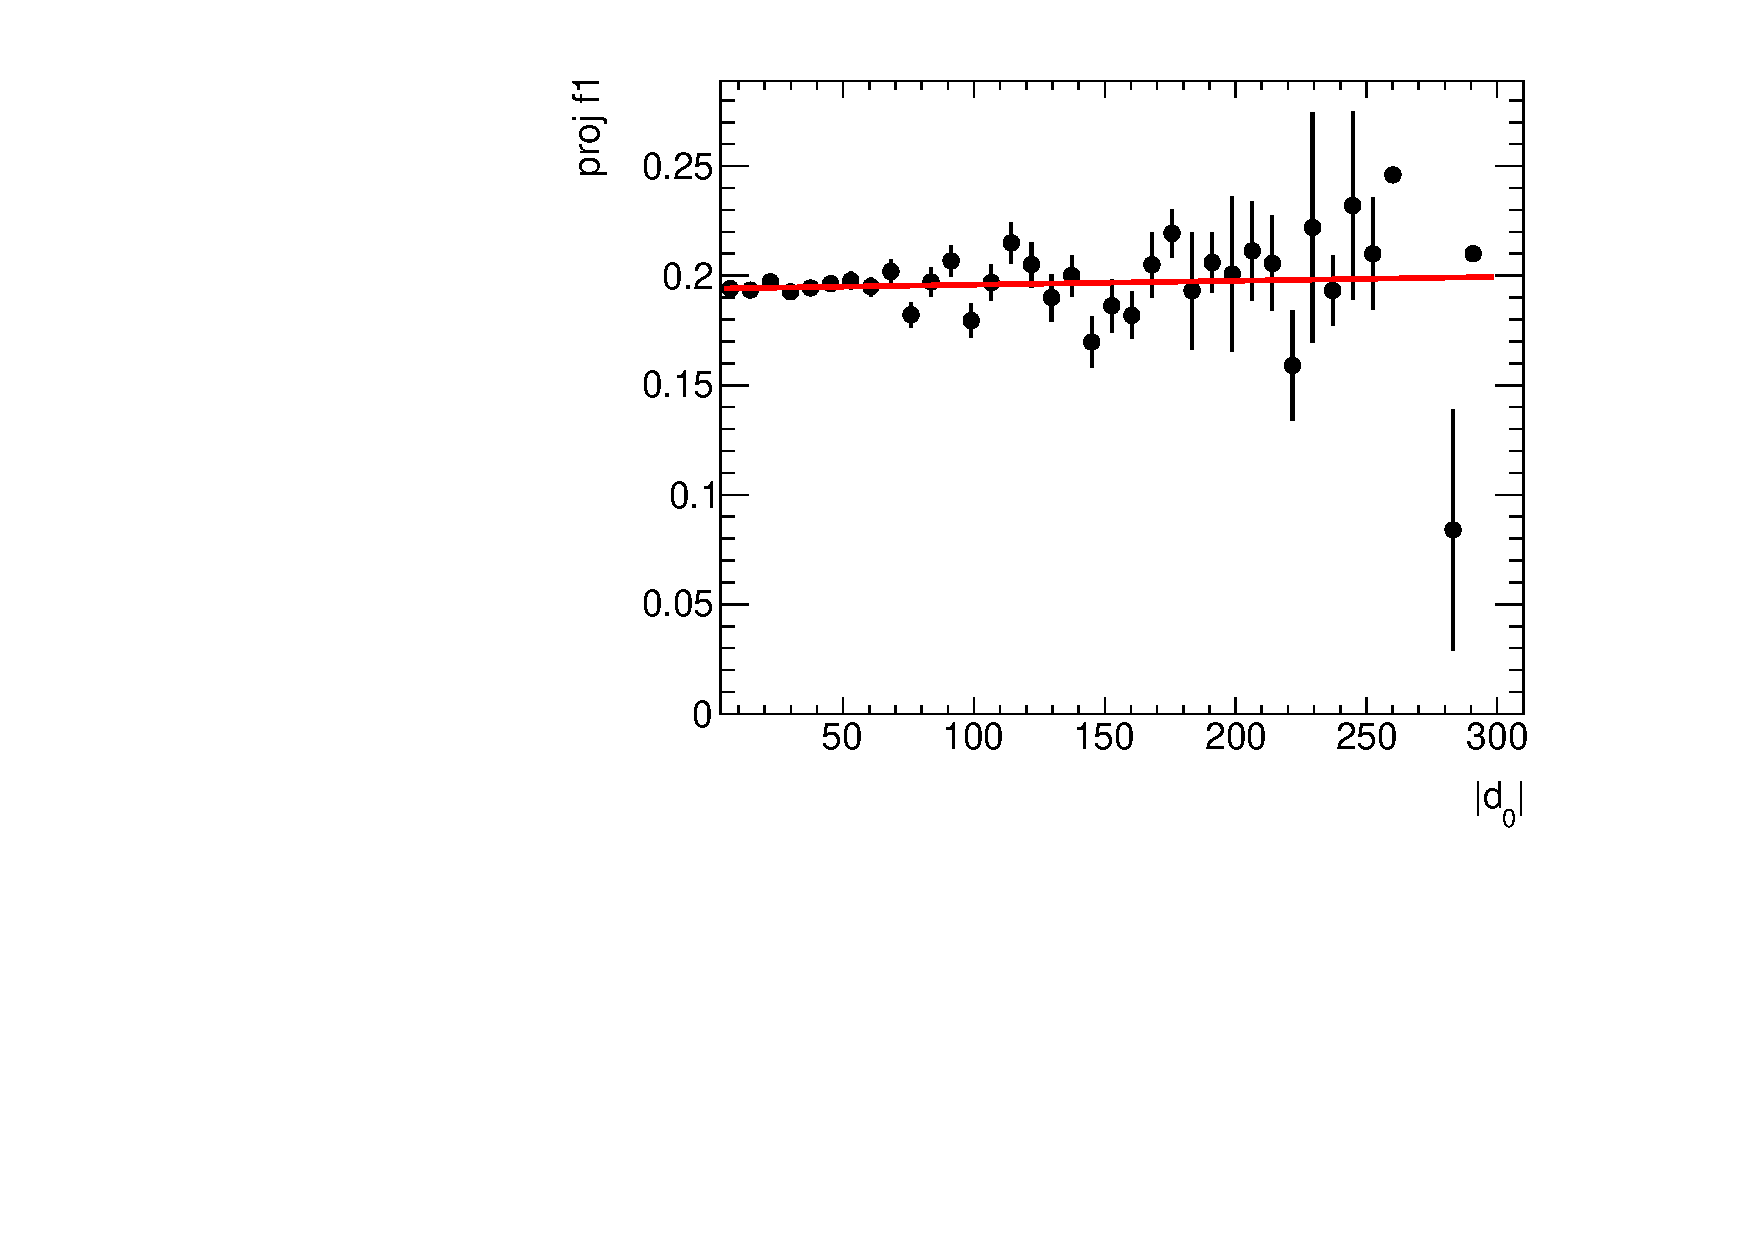
\includegraphics[width=.48\textwidth]{figures/disp_systs/e_signal_f1_profile.pdf}
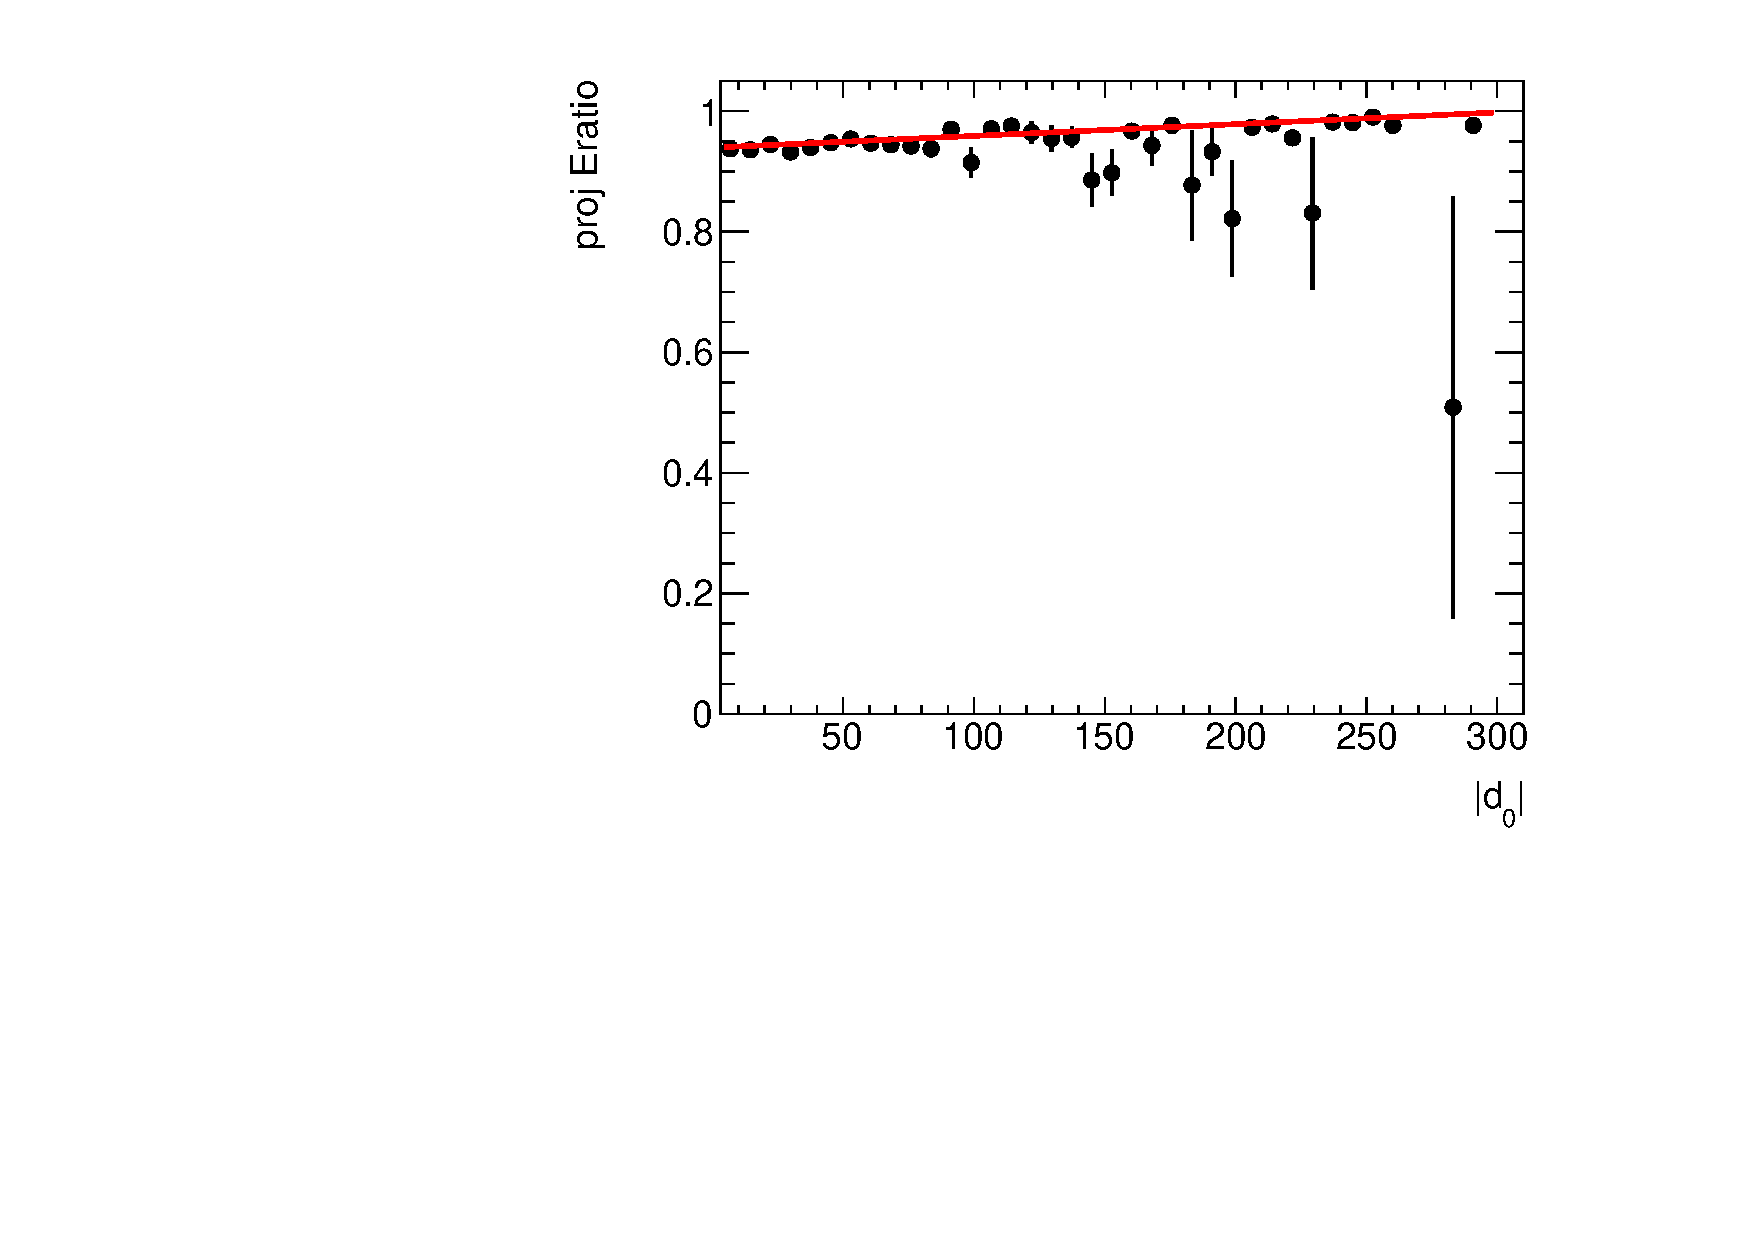
\includegraphics[width=.48\textwidth]{figures/disp_systs/e_signal_Eratio_profile.pdf}
\caption{Electron shower shape quality variables with trends with respect to \absdz, $f_{1}$ (left) and ERatio. Taken from a 300 GeV signal sample with lifetimes between 0.01ns-1ns.}
\label{fig:profs_el}
\end{figure}


\subsection{Other Sources of Uncertainty}

\subsubsection{Pileup Modeling}
When \ac{MC} is generated, particularly when it is generated during the course of the run, the actual pileup distribution of the events from the \ac{LHC} is not known. This is corrected through a process called \emph{pileup reweighting}, where a more realistic pileup profile is added to \ac{MC} events. Since the regions in this analysis are dominated by fakes and cosmics, not the kinds of events the pileup reweighting is trained for, the pileup modeling becomes a dominant uncertainty in this analysis.

\subsubsection{Theoretical Uncertainties}

Additional uncertainties are taken for the renormalization and factorization scales that are used to generate the physical processes in \ac{MC}. These impact both the cross section measurement and the final lepton kinematics. Both scales are varied, impact on the final results quantified, and the range of variation is taken as an uncertainty, in this analysis about 5\%. 

\subsubsection{Luminosity Measurement}
\ac{ATLAS} measures luminosity using dedicated detectors and calibrations (discussed in \autoref{sec:lumi}. The uncertainty on this measurement contributes a 2\% uncertainty to the analysis, as it impacts the normalization of the signal yield from \ac{MC}.




